\documentclass[uulm-release-print]{template/thesis-uulm}
% options:
% - uulm-draft: show to-do-notes, links, linenumbers hide label names
% - uulm-draft-verbose: show to-do-notes, links, linenumbers, label names
% - uulm-release-electronic: show links, hide to-do-notes, linenumbers, label names
% - uulm-release-print hide everything

% workaround for some stupid error in combination with IEEEtran, bibtex and babel
\makeatletter
\def\markboth#1#2{%
  \def\leftmark{\@IEEEcompsoconly{\sffamily}#1}%
  \def\rightmark{\@IEEEcompsoconly{\sffamily}#2}}
\makeatother

\usepackage[english]{babel}
\usepackage{natbib}
\usepackage{verbatim}

\usepackage{xcolor}
\usepackage{xfrac}

\usepackage{multirow}
\usepackage{float}

\usepackage{algorithm2e}
\usepackage[theme=default-plain]{template/jlcode} % https://github.com/wg030/jlcode

\usepackage{amsthm} % for theorems, lemmas and proofs
\usepackage{amsmath}
\newtheorem{lemma}{Lemma} % if buggy, use \newtheorem{theorem}{Theorem}[section] \newtheorem{lemma}[theorem]{Lemma} instead or \newtheorem{lem}{Lemma}

\KOMAoptions{bibliography=totoc, listof=totoc}

% Capitalized Chapters etc
\renewcommand{\chapterautorefname}{Chapter}
\renewcommand{\sectionautorefname}{Section}
\renewcommand{\subsectionautorefname}{Subsection}
\renewcommand{\subsubsectionautorefname}{Subsubsection}
\renewcommand{\figureautorefname}{Figure}
\renewcommand{\tableautorefname}{Table}
\renewcommand{\lstlistingname}{Listing}
\renewcommand{\algorithmautorefname}{Algorithm}

% Fonts
\renewcommand{\sfdefault}{phv}
\renewcommand{\rmdefault}{phv}
\renewcommand{\ttdefault}{pcr}

% using - instead of * in itemize environment
\renewcommand\labelitemi{---}

\author{Rebekka Roßberg}
\title{Robustifying the Set Covering Machine with Disjunctive Normal Forms\\and Nominal Features}
\email{rebekka.rossberg@uni-ulm.de}
\matnr{1049562}
\degree{Software Engineering}
\type{Bachelor's Thesis}
\jahr{2022}
\gutachterA{Prof.\ Dr.\ Hans A. Kestler}
\betreuer{Prof.\ Dr.\ Hans A. Kestler}

\begin{document}

\frontmatter %%%%%%%%%%%%%%%%%%%%%%%%%%%%%%%%%%%%%%%%%%%%%%%%%%%%%%%%%%%%%%%%%%%%%%%%%%%%%%%

\pagenumbering{roman}
\begin{nolinenumbers}
  \maketitle
  \copyrightpage%
\end{nolinenumbers}

\setstretch{1.2}

\begin{nolinenumbers}
  \tableofcontents
\end{nolinenumbers}

\mainmatter%%%%%%%%%%%%%%%%%%%%%%%%%%%%%%%%%%%%%%%%%%%%%%%%%%%%%%%%%%%%%%%%%%%%%%%%%%%%%%%%%

\pagenumbering{arabic}

\chapter{Introduction}\label{ch:introduction}

% Motivation
The set covering machine, also known as `set cover machine' or `SCM', is designed to be a `general-purpose learning machine'~\citep[p.727]{marchand02}
for binary classification problems.
In this thesis I want to further extend and optimize the SCM, in order to obtain a robust algorithm for the classification of high-dimensional gene expression data.

% overall goal: robustification
Per definition, robust algorithms are supposed to provide reasonable models,
even for input data with a certain degree of variations and erroneous values~\citep{burgard},
caused for example by measuring errors that often occur in real-world data sets.
While a robustification is often done by using the paradigm of linear programming to approach the problem, as in~\cite{hussain},
I cannot rely on hard error bound and will therefore approach the robustification from a more general point of view.
Here, the SCM is robustified mainly by the introduction of disjunctive normal form formulas as a
\textbf{way to construct more complex decision rules}.
Classification rules in disjunctive normal form are created by linking the logical ANDs, i.e.\ the conjunctions, with a single logical OR, i.e.\ a disjunction,
and therefore building a disjunction of conjunctions.
This extension seems especially promising for enhancing the classification of disjunctly scattered data.
Moreover the SCM is extended so it can handle not only numerical, but also categorical, features.
This \textbf{widens the potential application field of the SCM} by a lot, as data sets with categorical or even mixed
feature types can now also be processed.\
This extension was done in other research before, however, I will introduce some new modifications to further improve
the algorithm's performance on the various feature types.

The final classification rules will be in the form of, for example, `\texttt{IF (x1 < 3 AND x5 = `red') OR (x23 > 7.2 AND x2 = true) THEN class 1 ELSE class 0}'\\
and shall provide accurate predictions of the sample's labels without overfitting the test data.
Such an overfitting happens when the model perfectly covers the training data, yet is generalizable only
to a very small degree and therefore has a high risk of misclassifying independent test samples~\citep{drouin16}.
In the end, I want to be able to conduct a precise binary classification of oncological RNA sequencing data using the modified SCM.\
This use case scenario usually represents a major challenge for classification algorithms, as
gene expression data has an extremely high feature dimension, while at the same time, often only few samples are available.
Yet, the SCM can actually work comparatively well under such circumstances
and is able to perform a drastic feature reduction, in order to produce a compact and easy to interpret classification rule.

% Thesis' structure/ Overview
The thesis is structured as follows.
After introducing the concept of the set covering machine in \autoref{ch:scm},
the SCM is implemented in Julia and subsequently performance optimized in \autoref{ch:julia}, in order to
make the algorithm accessible, even for large data sets.
In \autoref{ch:dnf} and \autoref{ch:varFeat} the SCM is then extended and those
extensions are optimized optimized regarding both, the result's performance and the run time performance.
In these early chapters, artificially generated data sets are used exclusively to reason any decisions on evaluating and optimizing the algorithms.
Visualizations are provided for two-dimensional example sets.
Each of the data sets represents a specific scenario, such as two completely disjunct sample regions.
However, to test the algorithm's run time, randomly generated data was used, where each of the 200 samples is defined
as a vector \(X \in \lbrace0,1\rbrace^{50,000}\).
In \autoref{ch:evaluation} a total of nine data sets, that originate from
the UCI machine learning repository, as well as the cancer genome atlas, are introduced.
With those, a final evaluation of the modified SCM is executed and it is determined whether the algorithm
is actually capable of generating accurate and generalizable decision rules for real-world problems,
that separate crucial features from unimportant ones.
\chapter{The Set Covering Machine}\label{ch:scm}

First presented by~\cite{marchand02}, the `Set Covering Machine' is an algorithm 
that extends the works of~\cite{valiant} and~\cite{haussler88} to conduct binary
classifications.
These classifications are in an `\texttt{IF \(b_1\) AND \dots AND \(b_n\) THEN class 1 ELSE class 0}'
syntax, using a small logical conjunction or disjunction~\citep{taudien}.
The main goal of the SCM is therefore to find, or at least to approximate, the underlying function that maps data samples to their classes
and thus to minimize the chance of incorrectly classifying an input~\citep{drouin16}.

As the SCM is a supervised machine learning algorithm~\citep{haussler88}, it follows the schema depicted in \autoref{fig:learning_structure}.
It first produces a model, the classification rule, by learning on labeled training samples.
Afterwards the algorithm shall be able to predict the classes of unlabeled test data.
For these predictions, the accuracy, that equals one minus the generalization error, as well as the
sensitivity, i.e.\ the fraction of correctly classified class 1 samples, and the specificity,
i.e.\ the fraction of correctly classified class 0 samples, can be characterized.

\begin{figure}[ht]
    \centering
    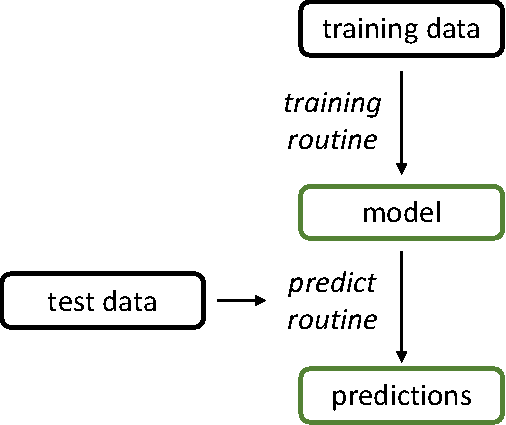
\includegraphics[width=0.55\columnwidth]{figures/learning_structure.pdf}
    \caption{General structure of a supervised learning algorithm. Inspired by~\cite{valiant}.}\label{fig:learning_structure}
\end{figure}

In the following sections, the algorithm, the underlying greedy set cover (see \autoref{sec:setCover}) and the SCM's predecessors (see \autoref{sec:origin}) are outlined.
First, original SCM for classifying data with a binary set of features (\autoref{sec:basicSCM}) is described, followed by short
introductions to different base classifiers like data-dependent balls (\autoref{subsec:balls}) and rays (\autoref{subsec:rays}).

%%%%%%%%%%%%%%%%%%%%%%%%%%%%%%%%%%%%%%%%%%%%%%%%%%%%%%%%%%%%%%%%%%%%%%%%%%%%%%%%%%%%%%%%%%%%
\section{Motivation and Requirements to the SCM}

% why no SVM?
While it seems like a good choice to just use the well-established support vector machine (SVM) by~\cite{cortes} for classification tasks, that might not always be the case.
The SVM algorithm constructs hyperplanes, along which it separates the two classes of data~\citep{cristianini}.
However this use of mainly linear hyperplanes for classification, makes the resulting models
quite complex, stiff and unintuitive to interpret for humans~\citep{marchand02}.

% produce sparse classifiers
The aim of the SCM is instead to produce a very simple, sparse and thus easy to interpret classifier that
clearly demonstrates the importance of each feature~\citep{drouin16}.
Linear separability of the data shall not be a requirement for the classification algorithm to work correctly~\cite{marchand02}.
Conjunctions are perfect for this task, as they are especially easy to understand for humans.
Having a simple rule as the algorithm's result, is furthermore beneficial, as it makes the SCM extremely valuable for scientific purposes,
as those rules are comparatively easily validatable using literature or even lab-experience~\citep{drouin16}.
They might also expose or verify hypotheses, or even set off future research by providing new insights~\citep{kestler11}.

% balance between short and accurate needed
It is the overall goal of every supervised learning algorithm to obtain classifiers with low generalization errors,
i.e.\ a good performance on unknown, independent test data.
To achieve such a low generalization error, both, the sparseness and the training accuracy of the decision rule, should be be maximized~\citep{marchand02}.
Yet, since the accuracy and the sparsity of a classifier are usually opposing goals~\citep{drouin16},
this is no easy problem and requires some elaborate balancing.
On the one hand side an extremely compact decision rule might only incorporate very few features and thus provide no feasible result at all.
On the other hand side, a very accurate classification rule might classify all test samples correctly, but come along with low interpretability and a
very high generalization error when applying the classifier to the test data.

% many features and few samples
Moreover, since the SCM is supposed to be a general-purpose learning machine,
the algorithm is in general able to deliver feasible results, even when confronted with a data set of a
very high feature dimension and low sample cardinality~\citep{kestler11}.
As data sets with tens of thousands of features and only a few hundred samples are not uncommon
in real-world problems and especially in biomedical learning tasks~\citep{lausser20}.
Yet the SCM is only expected to deliver good results, when very few features are actually informative.
This, however, is a minor requirement, since it is usually the case in real-world data sets.
The aim of the SCM is hence to bring order to this huge chaos of relevant and irrelevant features,
by picking only the few most relevant ones and forming them into a sparse logical conjunction, or disjunction, that is ordered by the features relevance,
as the most important feature is supposed to be added to the decision rule first~\citep{marchand02}.

%%%%%%%%%%%%%%%%%%%%%%%%%%%%%%%%%%%%%%%%%%%%%%%%%%%%%%%%%%%%%%%%%%%%%%%%%%%%%%%%%%%%%%%%%%%%
\section{Definitions}\label{sec:definitions}

% input space, classification rule
As its input, the basic SCM receives a binary data set \(S \in \lbrace0,1\rbrace^{m \times n}\) with
\(n\) attributes as its columns and \(m\) samples \(x \in \lbrace0,1\rbrace^{n}\) as its rows~\citep{marchand02}.
Additionally each sample has a label \(y \in \lbrace0,1\rbrace\).
Even though, as~\cite{schmid} showed, unlabeled samples could technically be incorporated into the training algorithm by using specific procedures,
this mechanism is not used in this thesis.
The goal of the SCM is now to find a good decision rule, also called `classifier' or `classification rule',
\(f: X \rightarrow Y = \lbrace0,1\rbrace\) that maps any sample of the input space \(X\) to its corresponding label \(y \in Y = \lbrace0,1\rbrace\).
% classification rule = set of multiple classifiers?!
The sample's classes, namely usually `class 0' and `class 1', will also be referred to as the `negative' and `positive' samples.

% attributes vs features
~\cite{marchand02} furthermore differentiate between `attributes' and `features'.
While attributes are usually Boolean valued, features can be of a more complex form.
Besides Boolean features, there are various other kinds of features such as rays (\autoref{subsec:rays}) and balls (\autoref{subsec:balls}).
Those more complex types of features are usually data-dependent, meaning that they were constructed from the available training data.
But in the end, all these features are essentially characteristics --- like `\texttt{\(x_5\) = true}' in case of Boolean features --- a sample either does or does not have.
Thus features are defined by~\cite{marchand02} as functions that evaluate to true or false given any sample \(x \in X\).

% base classifiers
On the other hand, `base classifiers' \(b_i\) are the first level (also known as `base' level) building blocks of the resulting classification rule~\citep{kestler11}.
`\texttt{\(x_9 < 7\)}' could for example be one of them, in case rays are used as base classifiers. % otherwise: base classifier = feature type

%%%%%%%%%%%%%%%%%%%%%%%%%%%%%%%%%%%%%%%%%%%%%%%%%%%%%%%%%%%%%%%%%%%%%%%%%%%%%%%%%%%%%%%%%%%%
\section{The Greedy Set Cover}\label{sec:setCover}

The minimum set cover problem on the data set \(S \in \lbrace0,1\rbrace^{m \times n}\) of m samples and n attributes is defined as follows.
It tries to cover each of the samples by at least one of the available attributes, each covering 0 to m of those elements.
A column j `covers' an element i, if and only if \(s_{ij} = 1\).
Additionally there usually is a cost vector \(c \in \mathbb{R}_{+}^{n} \) that associates a cost value to every column.
In the context of the SCM, the cost of every attribute is however set to one.
The goal of the set cover problem is now to find a subset of attributes that is of minimal cost and covers all m samples at least once~\citep{caprara}.

There are multiple ways of finding such a minimum set cover, that can be assigned mainly into the classes of exact, linear and heuristic algorithms~\citep{caprara}.
As the set cover problem is NP-complete, exact algorithms are barely realizable in the context of big data sets, because of their high worst case execution time bounds~\citep{chvatal}.
However, there exists an easy approach using a greedy heuristic, that has only polynomial worst case execution time introduced by~\cite{chvatal}.
A greedy algorithm in general solves an optimization problem by using the simple principle, 
of always choosing the current optimum for iteratively extending the solution.
This technique usually involves a loss of outcome optimality, hence the solution is usually only an approximation of the optimum,
yet, the algorithm benefits from a very fast computation time and often still results in feasible results~\citep{cormen}.

\begin{algorithm}[ht]
    \KwIn{S}
    uncovered samples = every line of S\\
    cover = \(\emptyset\)
    \While{uncovered samples \(\neq \emptyset\)}{
        Select attr \(\in\) S that covers the highest number of uncovered samples.\\
        uncovered samples = uncovered samples - attr \\
        cover = cover \(\cup\) \{attr\}
    }
    Return cover.
    \caption{The greedy set cover algorithm, as described by~\cite{chvatal}.}\label{code:greedySetCover}
\end{algorithm}

The `greedy set cover' algorithm, illustrated in \autoref{code:greedySetCover}, thus recursively selects the optimal sets.
After each iteration, it deletes the covered samples from the list of remaining ones.
Once all samples are covered, the algorithm stops and the subset of all selected sets is returned as the solution.
This greedy approach actually delivers a feasible minimum set cover with a proven, tight worst case bound that guarantees the
cost of the resulting greedy cover to be less than or equal \(H(d) \times \) the cost of the optimal cover~\citep{chvatal}.
Here \( H(d) = \sum_{i=1}^d \sfrac{1}{i} \) denotes the harmonic numbers with the size \(d\) of the largest set as its parameter.

%%%%%%%%%%%%%%%%%%%%%%%%%%%%%%%%%%%%%%%%%%%%%%%%%%%%%%%%%%%%%%%%%%%%%%%%%%%%%%%%%%%%%%%%%%%%
\section{The SCM's Predecessors}\label{sec:origin}

The SCM has its earliest origins in the algorithm of~\cite{valiant} for PAC learning a conjunctive binary classifier of Boolean attributes.
This approach was later optimized by~\cite{haussler88}, who reduced the classifier's complexity by applying the greedy set cover.

The following section gives a summary of the advancements and problems of early conjunction and disjunction learning algorithms.
All the algorithms in this section are applicable to both, conjunctions and disjunctions.
The disjunctive case can simply be obtained by switching the roles of the positive and negative training samples and applying trivial logical equivalences.

%%%%%%%%%%%%%%%%%%%%%%%%%%%%%%%%%%%%%%%%%%%%%%%%%%%%%%%%%%%%%%%%%%%%%%%%%%%%%%%%%%%%%%%%%%%%
\subsection{Valiant's Algorithm for Learning Conjunctions}

In his paper `A Theory of the Learnable'~\cite{valiant} introduced the concept of probably approximately correct (PAC) learnability.
He categorizes certain classes of binary classification problems as PAC learnable and constructs a two-step machine for PAC learning these problems in a supervised manner
with the goal of approximating their underlying classification functions at a high probability.
In this algorithm the teacher first gives the learner access to training samples using a specific learning protocol.
Here the learner can request randomly chosen positive samples or get the classification of an own sample to verify its tendencies.
In the following deduction procedure the learner now uses its knowledge from the learning first phase to derive a concept in the form of a Boolean function/expression.

Even though the resulting PAC classifier is not guaranteed to be correct, it is guaranteed to have a sensitivity of 100\% and a specificity \(< \varepsilon \)
forcing the probability of a false negative to be adjustable low, provided there are enough training samples available to the learner (precise bounds can be found in~\cite{valiant}).
This deduction procedure runs in polynomial time and thus forms a wide-spread base framework for developing efficient and probably correct learning algorithms~\citep{haussler90}.

~\cite{valiant} subsequently applies this PAC approach to constructing an algorithm to learn a conjunction or disjunction of Boolean attributes.
This algorithm uses the training samples to find a \(C \subseteq H\) containing exactly those attributes of the attribute set \(H\)
that correctly classify all of the positive training samples~\citep{marchand02}.
The conjunction of any \(c \in C\) is therefore also correctly classifies all positive training samples, giving each conjunction a sensitivity of 100\%.
To now also achieve the best possible results on the negative training samples, the conjunction of all \(c \in C\)  is formed and returned
as the chance of classifying a sample, that's not included in the set of positive samples, as negative
and therefore increasing the rules specificity, rises with every term that is added to the conjunction.
Yet this final decision rule is not guaranteed to be consistent with all of the negative samples or any of the unknown test samples.

However the requirement for a attribute to be consistent with all positive samples leads to an overfitting of the classifier
and wastes potential by not taking the negative samples into account~\citep{haussler88,marchand02}.
Additionally, the resulting conjunction may depend on a great number of attributes.
This high complexity most often leads to a decreased interpretability of the classifier,
as well as a high generalization error on unknown test samples.

%%%%%%%%%%%%%%%%%%%%%%%%%%%%%%%%%%%%%%%%%%%%%%%%%%%%%%%%%%%%%%%%%%%%%%%%%%%%%%%%%%%%%%%%%%%%
\subsection{Haussler's Two-Step Algorithm for Learning Sparse Conjunctions}

~\cite{haussler88} recognized the increased generalizability of compact classifiers and thus extended Valiant's algorithm accordingly.
In a two-step algorithm he first executes Valiant's algorithm to PAC learn a set \(C\) of Boolean attributes
that are all consistent with every sample.
As the second step he then uses the greedy set cover, with its tight bounds regarding the results accuracy and the execution time,
to reduce this attribute set to its smallest possible subset \(R \subseteq C\).
The conjunction of the subset's attributes has to correctly classifies all negative training samples, in order for \(R\) to be a valid solution.
If such a set does not exist, which happens quite often when working with complex real-world data, it returns no solution at all.
Yet whenever there actually exists set of attributes that is consistent with all training samples, 
Haussler's algorithm is guaranteed to find such a set as the solution~\citep{marchand02}.
Even more, this greedily obtained solution will be found in a time that is only polynomial in terms of \(n\) and \(m\)~\citep{kestler06}.
The classifier itself is bounded to be only by a factor of \(\ln m\) bigger than the optimal set of attributes \(s\)~\citep{marchand04,kestler06}.

Moreover this means, that the classifier's size does not depend on the total number of attributes \(n\), but only on the
number of relevant attributes \(s\), allowing the algorithm to perform well even if \(m << n\), as long as \(s \approx m\)~\citep{kestler06}.
In the end, the algorithm Haussler's algorithm returns a conjunction as the decision rule that is far more compact
than the original conjunction of Valiant and therefore has a way higher chance of a good generalizability.

But after all, the algorithms of~\cite{valiant} and~\cite{haussler88} have two major downsides:
Firstly they only work with Boolean attributes and secondly there is no possibility to adjust the level of the tradeoff
between the classifier's accuracy in training and its complexity~\citep{marchand02}.
Yet, this tradeoff is badly needed, as real-world data usually contains a lot of noise that can only be
filtered out by reducing the conjunctions accuracy and therefore improving the models ability to generalize~\citep{marchand02}.
To address these problems~\cite{marchand02} created the `set covering machine' algorithm.

%%%%%%%%%%%%%%%%%%%%%%%%%%%%%%%%%%%%%%%%%%%%%%%%%%%%%%%%%%%%%%%%%%%%%%%%%%%%%%%%%%%%%%%%%%%%
\section{The Basic Set Covering Machine}\label{sec:basicSCM}

~\cite{marchand02} generalized and extended Haussler's two-step algorithm by introducing the model selection hyper-parameters \(p\) and \(s\).
The penalty for misclassifying a positive sample \(p\) allows the users to control the trade-off between making errors on positive versus on negative samples.
On the other hand the early stopping point \(s\) lets them trade-off between an accurate classifier,
that is consistent with as many samples as possible, and a sparse classifier, that is easy to interpret and more generalized.
Additionally he replaced the Boolean attributes by Boolean valued features (see \autoref{sec:definitions}) that may be more complex, than ordinary attributes. 

The precise adjusting of the hyperparameter \(p\) comes in very handy, as both, conjunctions and disjunctions, have heavily asymmetrical behaviors.
A sample will only be classified as positive by a conjunction, if it is consistent with all base classifiers.
However, inside a disjunction, a sample will be classified as positive, once it is consistent with even just a single base classifier~\cite{schmid}.
In the case of a conjunction \(p\) should therefore usually prioritize the correctness of positive samples by being \(> 1\),
thus leading to an increased sensitivity of the the base classifier.
In the case of a disjunction the opposite should occur.
In addition \(p\) can also be used for balancing the classifiers sensitivity and specificity
depending on the ratio of positive training samples to negative training samples.
In the corner case of \(p = \infty\), a features has to be consistent with all positive samples in order to be selected,
like in Haussler's original algorithm~\citep{kestler06}.

The BuildSCM algorithm (\autoref{code:buildSCM}) has a worst case runtime complexity of only \(\mathcal{O} (m \cdot |H| \cdot s)\)~\citep{drouin16},
making it high performant even on large data sets.
When building a conjunction, a sample is removed from all remaining sets within the algorithm and requires no further consideration,
once it is classified as negative by a selected feature \(h_k \in Res\), as it has no chance to be reclassified anymore.
The same happens to samples that get classified as positive when constructing a disjunction.

The expression `\(|Q_i| - p \cdot |R_k|\)' quantifies a feature's usefulness~\citep{marchand02}.
This score however changes dynamically whenever a new, especially useful, feature is picked greedily as the next base classifier in every iteration,
as the feature's sets \(Q\) and \(R\) get effected directly.
The selection of a feature therefore always depends on the selection of the previously chosen features.
Yet, the selected feature \(h_k \in H\) may remain in \(H\),
as both \(Q_k\) and \(R_k\) are now empty sets anyhow, meaning that \(h_k\) will never again
have a usefulness score other than zero and thus will never be considered for \(Res\) anymore.
Once every negative sample \(n \in N\) is covered or \(s\) iterations have been executed
the resulting classification rule, here a simple conjunction or disjunction of Boolean features, is returned.

\begin{algorithm}[ht]
    \KwIn{
        \\ \(S\) --- training data set
        \\ \(p\) --- penalty value for a misclassification
        \\ \(s\) --- maximum amount of base classifiers that may be used in the rule
        \\ \(H\) --- set of Boolean valued features \(h_i(x)\)}
    \KwOut{sparse conjunction/ disjunction of \(Res \subseteq H\)}
    \(Res = \emptyset\) \\
    \(P =
    \begin{cases}
        \text{set of positive training samples,} & \text{conjunctive SCM} \\
        \text{set of negative training samples,} & \text{disjunctive SCM}
    \end{cases}\) \\
    \(N =
    \begin{cases}
        \text{set of negative training samples,} & \text{conjunctive SCM} \\
        \text{set of positive training samples,} & \text{disjunctive SCM}
    \end{cases}\) \\
    \For{\(h_i \in H\)}{
        \(Q_i\) = subset of \(N\)'s elements that are consistent with the assumption of \(h_i\) \\
        \(R_i\) = subset of \(P\)'s elements that are inconsistent with the assumption of \(h_i\)
    }
    \While{\(|N| > 0\) and \(|Res| < s\)}{
        \(h_k\) = feature \(h_i \in H\) with the maximum value of \(|Q_i| - p \cdot |R_k|\) \\
        \(Res = Res \cup \{h_k\}\) \\
        \(N = N - Q_k\) \\
        \(P = P - R_k\) \\
        \For{\(h_i \in H\)}{
            \(Q_i = Q_i - Q_k\) \\
            \(R_i = R_i - R_k\)
        }
    }
    Return \(f(x) =
    \begin{cases}
        \bigwedge_{i \in Res} h_i(x), & \text{conjunctive SCM} \\
        \bigvee_{i \in Res} h_i(x), & \text{disjunctive SCM}
    \end{cases}\)
    \caption{The basic `BuildSCM' algorithm for Boolean features. Created according to~\cite{marchand02}.}\label{code:buildSCM}
\end{algorithm}

The SCM always only approximates the optimal solution, as it is using a greedy algorithm.
Nevertheless~\cite{marchand02} observed, that if there actually exists a sparse conjunction or disjunction with few errors on the training data,
the correctly adjusted BuildSCM algorithm will most likely identify this classifier.
This further implies that the algorithm performs well, even when working on a data set with far more features than samples,
provided that only few of those features are actually relevant for a classification.
Overall the SCM benefits highly from its simplicity, both of the algorithm itself and the resulting classifiers,
and the high compression rate that is achieved by compression the main information of a huge data set into
just a small rule, that can even be stores as a simple string.

%%%%%%%%%%%%%%%%%%%%%%%%%%%%%%%%%%%%%%%%%%%%%%%%%%%%%%%%%%%%%%%%%%%%%%%%%%%%%%%%%%%%%%%%%%%%
\section{Extending the SCM by Different Base Classifiers}\label{sec:baseClassifiers}

Besides this SCM for Boolean features with classification rules like `\texttt{IF x1 AND x4 THEN class 1}',
there are many different types of base classifiers that can be employed for the decision rules~\citep{kestler11}.
The data set is now in general defined as \(S \in \mathbb{R}^{m \times n}\), instead of only \(S \in \lbrace0,1\rbrace^{m \times n}\).
This makes the SCM easily applicable to a whole new group of real-world data sets, like gene expression data.
Good base classifiers shall have good compression rates,
meaning that they reduce the dimension of the data set by a lot by encoding the information into a more compact notation.
This compression rate is usually measured as the ratio of the SCM's input, the sample set, to its output, the classifier.
It assumes that the algorithms output contains all important sample information.

Since data-dependent balls and data-dependent rays can be considered as the two most promising and widespread base classifiers,
their concepts are introduced in the following.
But there are many more noteworthy types of base classifiers like data-dependent half spaces 
that~\cite{marchand03} developed as an extension to the concept of data-dependent balls.

%%%%%%%%%%%%%%%%%%%%%%%%%%%%%%%%%%%%%%%%%%%%%%%%%%%%%%%%%%%%%%%%%%%%%%%%%%%%%%%%%%%%%%%%%%%%
\subsection{Using Data-Dependent Balls as Features}\label{subsec:balls}

~\cite{marchand02} first introduced the concept of having a set of spheres, that are centered around training samples, as the set of features.
The SCM here successively selects the most favorable balls, according to a specific heuristic, for the resulting conjunction or disjunction~\citep{germain}.
Using the PAC framework,~\cite{marchand02} give a tight bound for the generalization error of this SCM
in terms of the achieved amount of sample compression.

Each feature
\[h_{i,p}(x) \mathrel{\mathop:}= h_p(x,x_i) =
\begin{cases}
    y_i, & d(x,x_i) \leq p \\
    \overline{y_i}, & else
\end{cases}\]
is defined as the inside of a sphere around one training sample \(x_i\) with the radius \(p \in \mathbb{R}\) and
the distance \(d(x,x_i)\) between the points \(x\) and \(y\), that may be calculated using any common distance metric~\citep{marchand02}.
A sample is therefore classified using its proximity to other samples~\citep{germain}.
This however leads to a very complex model, as the distances of every feature to every other feature need to be computed and stored,
making the runtime complexity of this SCM with data-dependent balls exponential in the number of samples and therefore very high.

%%%%%%%%%%%%%%%%%%%%%%%%%%%%%%%%%%%%%%%%%%%%%%%%%%%%%%%%%%%%%%%%%%%%%%%%%%%%%%%%%%%%%%%%%%%%
\subsection{Using Data-Dependent Rays as Features}\label{subsec:rays}

Shortly after the concept of building an SCM that uses data-dependent rays as its set of features was first introduced by~\cite{marchand04},
~\cite{kestler06} picked it up, extended it and used for microarray analyses.
The application of this SCM type on gene expression data, or in general many types of real-world data with real-valued features, works very well and
provides valuable information on the underlying patterns by its simple and easily to interpret classification classification rules~\citep{marchand04,kestler06,kestler11}.
Moreover it works well on data of high feature dimension and low cardinality, in which case there is a high
chance of one ray being perfectly consistent with all samples.
I will therefore use these data-dependent rays for the following analysis of high-dimensional RNA-seq data.

A `single threshold classifier' (STC) is defined as a classifier, that predicts the label of a sample,
according to a single threshold \(t\), that only depends on a single feature \(h_i \in \mathbb{R}\) of the sample \(x_j\)~\citep{kestler11,marchand04}.
`x5 = 4.1' could for example be such a STC.\
Rays use these STCs and expand them by a direction to produce rules in the form of `\(\text{feature}_x \geq \text{threshold}_y\)' and `\(\text{feature}_x < \text{threshold}_y\)'~\citep{marchand04}.
This direction can for example be be defined binary as \(d \in \{-1,1\}\), allowing the definition of a ray as
\[r(x) =
\begin{cases}
    1, & (x_{ij} - t)d \geq 0 \\
    0, & else
\end{cases}\]~\citep{kestler11}.
According to~\cite{kestler11}, a ray is called `data-dependent', if its threshold is placed directly on top of a data sample.
In general the features are not input separately into the algorithm in form of a feature set \(H\), but are directly derived from the data set \(S\),
when using data-dependent rays.

% interval vs rays
As rays are basically half-open intervals~\citep{kestler11}, the conjunction of an ensemble of rays forms a, usually partially open, hyper-rectangle in the input space,
with the ray's thresholds being the hyper-rectangle's borders.
The SCM with rays as base classifiers is in general very high performant, even in the context of high-dimensional data sets~\citep{kestler11}.
~\cite{kestler06} bounded the generalization error of the SCM with data-dependent rays as its set of features based on the Vapnik-Chervonenkis (VC) dimension of the base classifier space.
Those bounds were then tightened by new error bounds, this time based on the amount of data compression this version of the SCM achieves on its training data.
~\cite{kestler11} furthermore constructs and proves a good sample compression bound for this version of the SCM.\
\chapter{Implementation in Julia}\label{ch:julia}

% framework
I first implemented a set covering machine with single threshold base classifiers, such as rays, in order to extend it in the following chapters.
This was done in Julia, a fast and simple structured programming language first presented in~\cite{bezanson}, in version 1.7.2.
Furthermore the packages `\texttt{CVS.jl}' and `\texttt{RData.jl}' to read CSV and RData files, in addition to
`\texttt{DataFrames.jl}' for the efficient and comfortable handling of data matrices, were employed.
In contrast to a usual Julia matrix, each column of a data frame has a distinct name, that can be set by the user.
`\texttt{PlotlyJS.jl}' was used as the graphing library for plotting the results and
`\texttt{BenchmarkTools.jl}' for benchmarking with the `\texttt{@btime}' macro to log execution times and used RAM spaces.

% good performance
After starting with the BuildSCM algorithm of~\cite{marchand02} with binary features as the fundament,
the basis algorithm is then adjusted and optimized for the computation in Julia, in order to improve its run time performance,
i.e.\ to minimize the algorithm's execution time and its RAM workload.
This is needed as, in the end, the SCM shall be capable of analyzing huge data sets with up to 50,000 features and a few hundred samples.

\section{Adjusting the BuildSCM Algorithm}

\begin{figure}[ht]
    \centering
    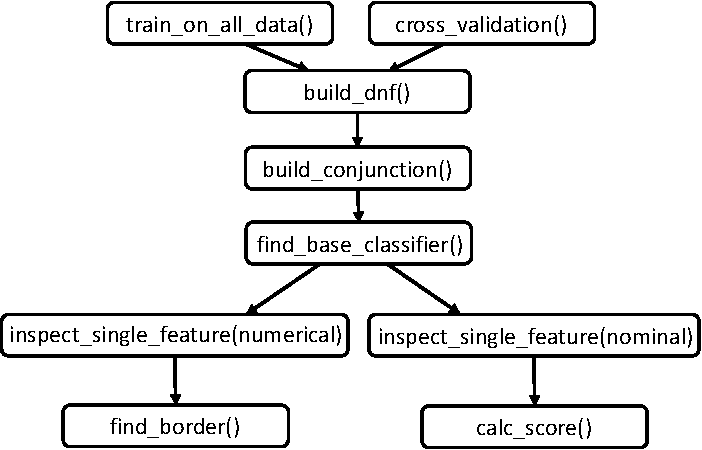
\includegraphics[width=0.85\columnwidth]{figures/training_structure.pdf}
    \caption{Structure of the training algorithm. \autoref{ch:dnf} will explain the need and details of the \texttt{build\_dnf} function. While \autoref{ch:varFeat} will explain the reasons for splitting the \texttt{inspect\_single\_feature} function.}\label{fig:training_structure}
\end{figure}

\begin{jllisting}[caption={Storing base classifiers as structs.}, label={julia:baseClassifier}]
    struct BaseClassifier
        featureId::Int32
        operator::Char
        threshold::Union{Float64, Int64, Bool, AbstractString}
        score::Float64
    end
\end{jllisting}

I structured my SCM training algorithm as displayed in \autoref{fig:training_structure}.
In contrast to the usage of a binary direction variable for rays like in the original algorithm of~\cite{marchand02}, a Julia struct `BaseClassifier' (see \autoref{julia:baseClassifier})
is now used to store each ray's attributes in a central, immutable and easy to understand structure.
As the rays's operator is stored as an arbitrary char, a function to interpret it, in the style of `\texttt{if operator == '\(\geq\)' then return value < threshold}', is needed additionally.
Yet, besides this and a slightly increased RAM and execution time demands, this form of storage comes with the huge advantage of being extendible to many different kinds 
of rays and even other base classifiers, for example for the integration of an `=' or an `>' operator, as done in \autoref{ch:varFeat}.

% low level to high level
For the calculation of each base classfier's usefulness score, implemented in \autoref{julia:calcScore}, 
the formula suggested by~\cite{marchand02} with a constant value for \(p\) is used and
no further investigations on other functions to calculate this score are performed.
However \(Q\) and \(R\) are computed adhoc, without the use of any \(N\) or \(P\), as done by~\cite{marchand02}.
In general, it is quite insufficient to handle \(Q\) and \(R\) as the real rows of the data matrix \(S\), as with this
method execution times skyrocket, already when dealing with slightly larger data sets.
The next option would be to handle \(Q\) and \(R\) in the form of indices that reference the corresponding lines of \(S\).
However this approach is also not feasible in the context of big data sets, as the constant storing,
transferring and updating of these parameters leads to way too much computational effort.
Instead it is best to simply recalculate the usefulness score together with \(Q\) and \(R\) whenever it is needed.
This decreases the code's RAM requirements from \(\mathcal{O}(|\text{features}| \cdot |\text{samples}| \cdot 2)\) for permanently storing the current Q and R indices
of all features for possibly all samples, to only \(\mathcal{O}(1)\) for storing the element with the maximum score at the time.

The best base classifiers are then collected and compared to each other on different tiers of the algorithm.
Finally, in each iteration the optimal classifier is chosen and incorporated into a classifier that works purely conjunctive.
The next iteration of the \texttt{build\_conjunction} function, depicted in \autoref{julia:buildConj},
then continues on the samples that were classified as positive by all previously selected base classifiers, as well as the new ones.
However, once a base classifier, that does not classify at least one positive and one negative
sample correctly, is selected as the new optimum, this classifier is discarded and the conjunction is finished right away.
This ensures that the conjunction will not grow without a good reason to do so.

\section{Performance Optimization}

% pretty code and efficient
In general great emphasis was put on creating compact, maintainable and well documented Julia code.
However, at the same time, the SCM was also designed to be as high performant as possible,
in order to be able to test it on huge data sets later on.
To achieve these goals, many performance optimized Julia features were used, such as multiple dispatch, Julia's version of function overloading,
anonymous parameters `\_' and a strong typing system that is used for all function parameters.

While using fixed-length tuples instead of vectors seemed promising at first, it did in fact not turn out
too well, as the data set is loaded from its original file as a data frame either way.
From this data frame, single vectors are easily extractable, but to obtain tuples, the corresponding vectors have to be
re-typed manually --- a process, which is quite performance intense.
Therefore mainly data frames and vectors were used in the end, yet there are still multiple ways to optimize them, like
referencing a column by using `\texttt{S[!, x]}' instead of copying it by `\texttt{S[:, x]}' and only passing essential
data to subfunction, like pre-extracted vectors or values.
Sets, instead of arrays, were employed wherever they were useful, in order to be able to use efficient Julia operations especially designed for sets, such as `\texttt{union}' and `\texttt{setdiff}'.
Those operations are in general faster than the the equivalent operations on arrays. 

% interpretable rules
Moreover I put effort in producing easy to interpret classification rules.
Instead of outputting confusing tables, like some other SCM algorithms do, my algorithm actually outputs
the whole rule in a human readable form like `\texttt{IF length < 5.1 AND height < 7.3 THEN will fit}'.
In these rules real feature names, instead of their their abbreviations, and real class names, instead of just `class 1' and `class 0',
were used.
This ensures that the SCM is able to produce rules that can eventually be supported or validated by science, as suggested~\cite{drouin16}.

However to keep the algorithm at high performant as possible, the calculations were done on the feature's indexes and Boolean class labels themselves and
the semantic details were solely solely when needed.
In case of the feature names, that task is done by the \texttt{to\_string} functions, as displayed in \autoref{julia:toString}.
This group of functions is also a prime example for the use of multiple dispatch.
For the class labels, on the other hand, the Julia function \texttt{booleanize\_labels!} (see \autoref{julia:boolLabels}) was used to extract the labels
from the loaded data and obtain a data frame with Boolean labels.
This data frame is then suitable for an ensemble of highly efficient vector operations and compact enough for quick transferring to various functions.

% Parallelization by multi threading
Furthermore parallelization was incorporated by starting Julia with the command `\texttt{julia --threads auto}'
and using the `\texttt{Threads.@threads for i in 1:m}'\\macro to activate multi threading in certain loops.
Within a multithreaded loop, it is important to ensure the independence of each iteration, i.e.\ if
a variable is manipulated by a thread, it may not be manipulated, or even read, by any other thread.
Therefore fixed width arrays were used, where every thread has its own array position that it can write to.

Within the SCM, parallelization was especially useful at the \(m \times n\) iterations of a cross-validation (see \autoref{sec:evalMethods})
and within the \texttt{find\_base\_classifier} function,
as in these use cases, every iteration constructs a model that is completely independent from all other iterations.
\texttt{Find\_base\_classifier} in particular collects the optimal base classifier of every feature, compares them and returns only the best, i.e.\ the highest scoring, of them.
Its multithreaded implementation can be found in \autoref{julia:findBaseClassifier}.
The parallelization drastically improves the algorithms runtime performance:
When executing the \texttt{build\_conjunction} routine with a randomly generated data set of 50,000 numerical features and 200 samples,
it needs about 22.734 seconds without and 8.855 seconds with multithreading used in the \texttt{find\_base\_classifier} function.
\chapter{Constructing Disjunctive Normal Form Expressions}\label{ch:dnf}

% definition and characteristics of DNF -> why is it so interesting
A disjunctive normal form (DNF) formula is defined to be a disjunction of at least one conjunction of at least one literal~\citep{aizenstein}.
Each literal is either a negated or a non negated variable. 
Moreover each variable can be interpreted as \(g: X -> \lbrace0,1\rbrace\), for any Boolean expression \(X\)~\citep{davey}.

% every function can be a DNF -> motivation
Every classification concept that is representable as a Boolean function, is convertible into an equivalent DNF,
using logical equivalences like for example the De Morgan's laws \(a \vee b = \overline{a \wedge b}\)~\citep{davey}.
Moreover DNFs are canonical normal forms of Boolean functions, meaning that every Boolean function has exactly one representation as a full DNF,
that is definite except for variations based on associativity and commutativity of the logical conjunctions~\citep{davey}.
Though, there is no guarantee for a DNF representation to be compact.
~\cite{aizenstein} prove that the correct DNF representation of a subject cannot only be found in exponential time,
but for large groups of issues even in only polynomial time.

% minimized DNFs
A DNF can be minimized using tools like Karnaugh maps or the Quine–McCluskey algorithm~\citep{allender}.
A classic minimization could for example be the summarizing of `\((a \wedge b)\vee(a \wedge \overline{b})\)' to `\(a\)'.
Even though the algorithm for finding the minimal DNF is NP-complete and will therefore not be implemented here,
the optional solution can be approximated by the greedily collecting the prime implicants and
always adding the conjunction to the disjunction next, that covers the most remaining positive samples~\citep{allender}.

% motivation
DNFs are widely spread in machine learning and still subject to further research,
as they provide easy to interpret decision functions as representations for many real-world concepts, even in complex scientific contexts~\citep{aizenstein}.
Whereas a conjunctive normal form formula is comparatively hard to interpret for humans, since it appears less often in nature.
Thus, I decided to extend the the conjunctive classification rules of the set covering machine into DNF expressions.
A `full DNF' furthermore would have every variable appear in every conjunction, however those special DNFs do in general not result from the SCM.\

% using DNFs in the SCM
So far the SCM only constructs pure conjunctions or pure disjunctions.
Yet, in classification tasks with disjunctly scattered samples, pure conjunctions are
unable to give accurate classifications and DNFs are strongly needed.
After commenting on the general concept and its Julia implementation in \autoref{sec:conc},
different approaches to optimize the \(SCM_{DNF}\) are presented:
first by adjustments on the input parameters (\autoref{sec:adjustingParam}) and later by
making use of equally optimal base classifiers (\autoref{sec:ties}).

%%%%%%%%%%%%%%%%%%%%%%%%%%%%%%%%%%%%%%%%%%%%%%%%%%%%%%%%%%%%%%%%%%%%%%%%%%%%%%%%%%%%%%%%%%%%
\section{Concept and Implementation}\label{sec:conc}

While, in the algorithm of~\cite{haussler88}, every sample is per definition correctly covered by the first conjunction,
canceling the need of having multiple conjunctions, with~\cite{marchand02} introducing the hyperparameter \(p\), this situation changed.
Now it is not uncommon anymore for a conjunction not to cover all positive samples.
By the use of an ensemble of conjunctions and the linking of those by one big disjunction,
more positive samples can be covered by the classification rule and feasible results can be achieved, even for data sets, as in \autoref{fig:twoReg}, with
extremely disjunct decision regions within a class.

\begin{figure}[ht]
    \centering
    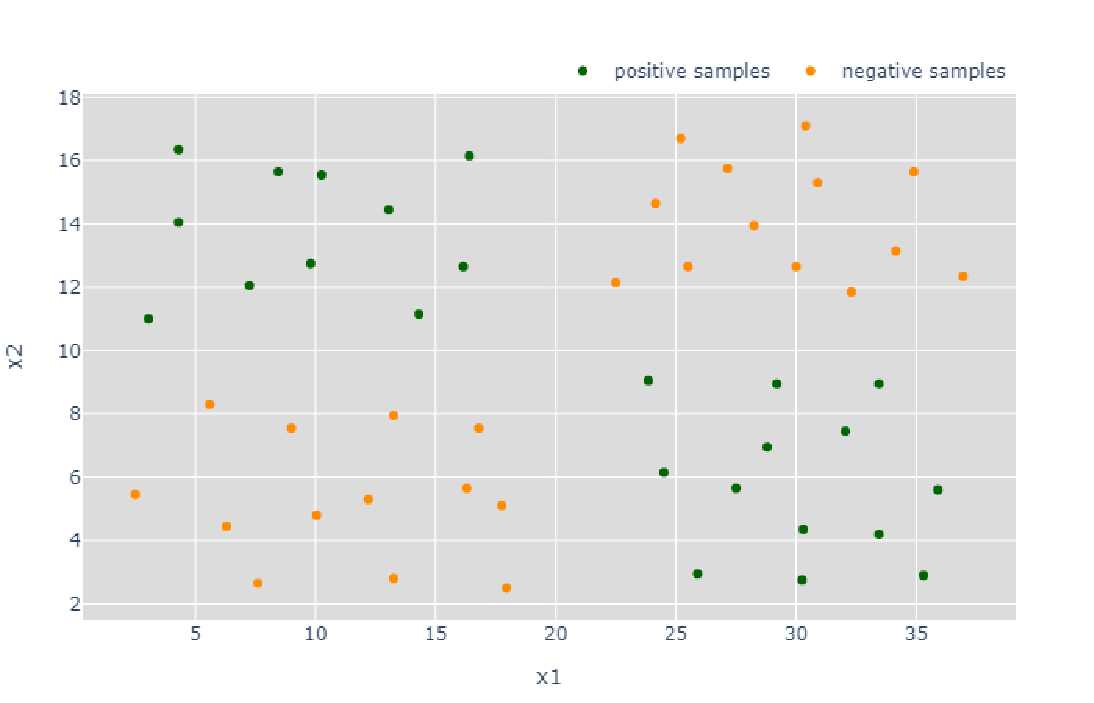
\includegraphics[width=0.85\columnwidth]{figures/two_reg.pdf}
    \caption{Data set with positive samples that scatter distinctly into two decision regions.}\label{fig:twoReg}
\end{figure}

The schematic algorithm to build DNF classification rules is depicted in \autoref{code:SCM_DNF}, its Julia implementation can be found in \autoref{julia:buildDnf}.
Here \(sC\) defines the maximum number of base classifiers within each conjunction and \(sD\) the maximum number of conjunctions within the disjunction.
\(minConjSize\) on the other hand sets a minimum usefulness requirement for conjunctions in order for them to be included into the DNF.\
The code of the conjunctive SCM can directly be integrated into this algorithm and in general does not need to be changed at all,
as the algorithm solely extends the conjunctive SCMs rule to a whole set of rules and thus creates an \(SCM_{DNF}\).
By the mechanisms of greedily picking optimal conjunctions for the disjunction, the generated DNF will even be in a somewhat, yet not
guaranteed to be optimal, minimal form~\citep{allender}.

\begin{algorithm}[ht]
    \KwIn{\(S\), \(p\), \(sC\), \(sD\), \(minConjSize\)}
    conjunctions = \(\emptyset\) \\
    \While{\(\exists\) misclassified positive sample AND length of conjunctions \(< sD\)}{
        conj = whole, and maximal big, conjunctive classifier generated by \autoref{julia:buildConj} with the parameters \(S\), \(p\) and \(sC\) \\
        Predict the labels of each sample using conj. \\
        \If{conj = \(\emptyset\) OR \{positive samples covered by conj\} < \(minConjSize\)}{
            Break loop.
        }
        \(S = S -\) positive samples covered by conj \\
        conjunctions = conjunctions \(\cup\) conj \\
    }
    Return conjunctions.
    \caption{Basic algorithm to build a DNF classifier from conjunctive classifiers.}\label{code:SCM_DNF}
\end{algorithm}

The \texttt{build\_dnf} algorithm is actually really similar to the algorithm of building a conjunctive SCM, with the main differences being
that conjunctions are collected, instead of single base classifiers, and in every iteration the samples that are classified as positive,
instead of negative, get deleted from the data set, as this classification is now final.
This is caused by the uneven behavior of conjunctions and disjunctions, that comes especially clear when observing
the ways each rule type classifies samples in \autoref{julia:classify}.
By placing conjunctions nested in a disjunction, the asymmetric behavior is somehow balanced.

%%%%%%%%%%%%%%%%%%%%%%%%%%%%%%%%%%%%%%%%%%%%%%%%%%%%%%%%%%%%%%%%%%%%%%%%%%%%%%%%%%%%%%%%%%%%
\section{Adjusting the Algorithms Parameters}\label{sec:adjustingParam}

To ensure that the algorithm is able to produce good results for various data sets,
the parameters \(p\), \(sD\), \(sD\) and \(minConjSize\), that can be adjusted independently, are implemented.

%%%%%%%%%%%%%%%%%%%%%%%%%%%%%%%%%%%%%%%%%%%%%%%%%%%%%%%%%%%%%%%%%%%%%%%%%%%%%%%%%%%%%%%%%%%%
\subsection{Early Stopping Points}

A DNF will usually perform better than a pure conjunction when it comes to classifying the training data, as it has more possibilities to cover the data points.
However that is not necessarily the case, when it comes to classifying unknown test data.
The possibility to link multiple conjunctions into a DNF gives the SCM the ability to extremely
over-fit the classifier to the training data --- way more than a normal conjunctive SCM ever could.
As overfitting of the training data leads to a high generalization error on test data and therefore
an overall bad performance of the classifier, it is crucial to find a good balance between high accuracies on
training data and high generalizability.

The input parameters \(sC\in \mathbb{N}\), \(sD\in \mathbb{N}\) and \(minConjSize\in \mathbb{N}\) are used to help with this exact problem.
They are early stopping points, meaning that they force the classification rule building process to stop,
even if there could still be a base classifier or conjunction added.
\(sC\) in particular limits the DNF to a k-NDF with \(k = sC\).
While \(sC\) and \(sD\) leads to a process termination simply by providing a hard upper limit to the maximum number of
base classifiers or conjunctions, \(minConjSize\) has the softer approach.
It stops the algorithm whenever an `optimal' conjunction is picked, covering so few positive samples, 
that it does not actually help with identifying a new decision region.

As the main goal is to find and characterize all decision regions of the data set, I focus on the use of the \(minConjSize\) parameter.
If the SCM is for example executed on a data set that actually has five disjunct decision regions, with ten positive samples each, along with some random scattering,
The algorithm should not terminate after it found \(n\) of those decision regions because \(sD\) forced it to stop.
Instead it is supposed to find all five regions and then stop, because the sixth region it found
is too small and loose to classify at least \(minConjSize\) additional positive samples as positiv.
As a consequence, both, \(sC\) and \(sD\), are in general set to the comparatively high standard value of 10 and
focus on the adjustment of \(minConjSize\).

\begin{figure}
    \centering
    \begin{subfigure}{\textwidth}
        \centering
        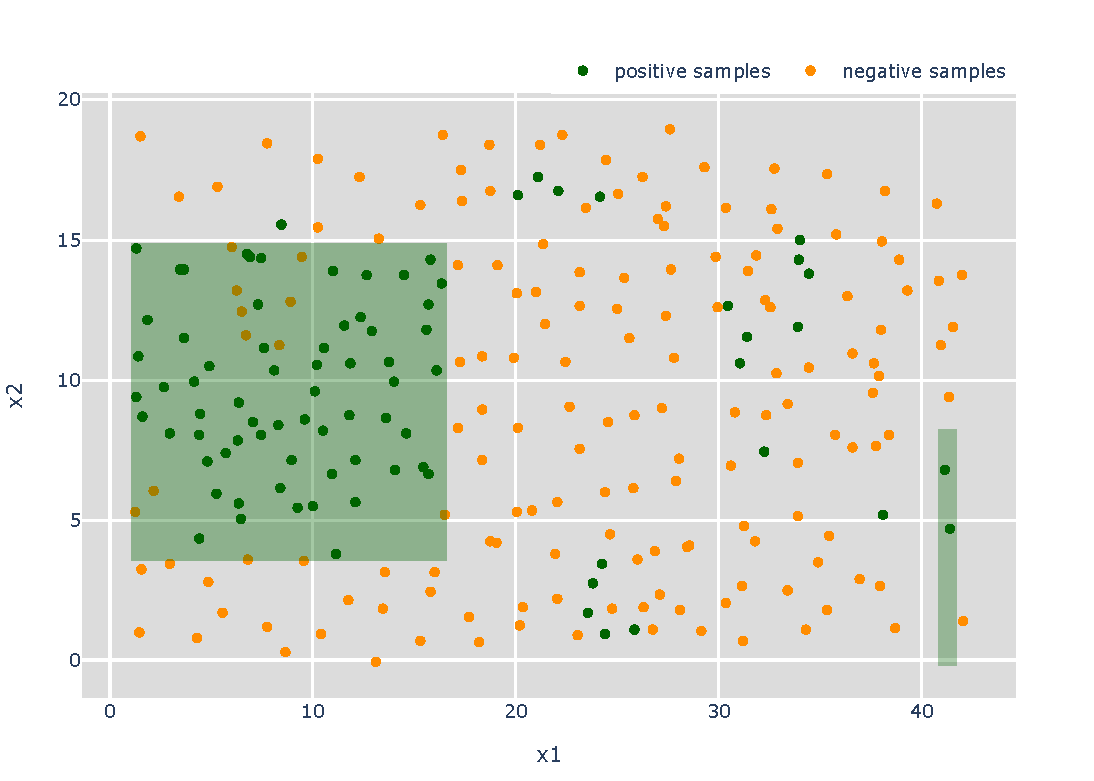
\includegraphics[width=0.85\columnwidth]{figures/complex_pattern_conj_size_1.pdf}
        \caption{\(minConjSize = 1\).}
    \end{subfigure}
    \hfill
    \begin{subfigure}{\textwidth}
        \centering
        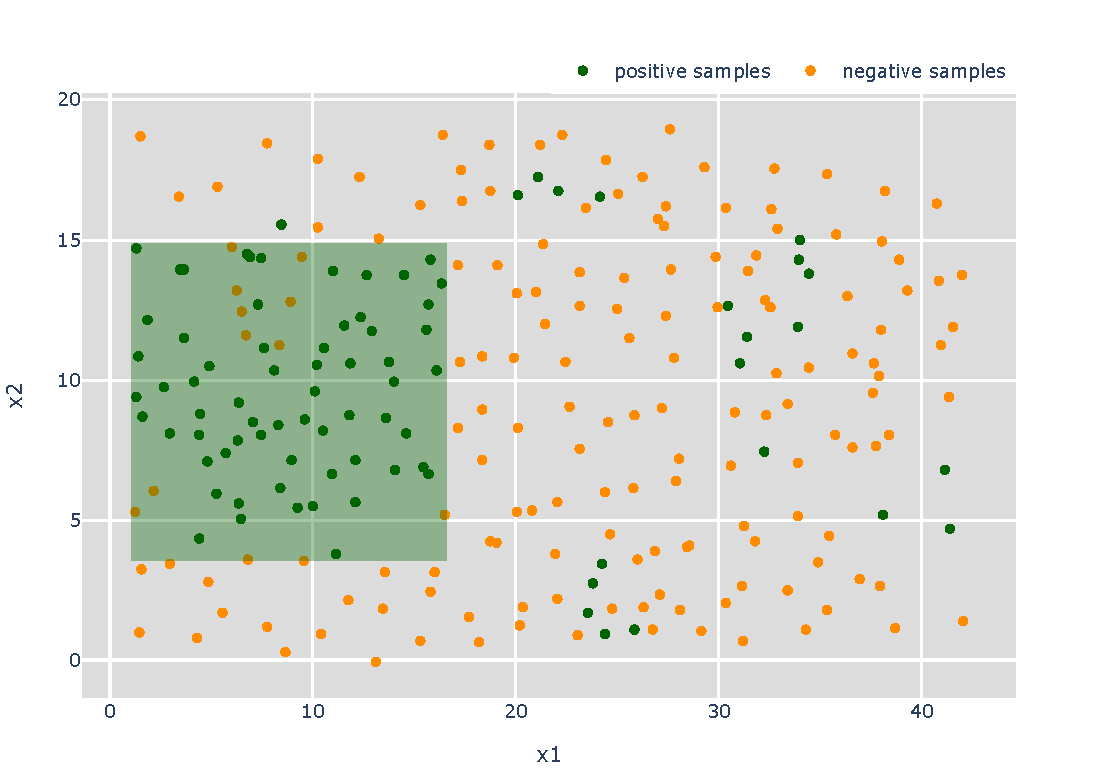
\includegraphics[width=0.85\columnwidth]{figures/complex_pattern_conj_size_5.pdf}
        \caption{\(minConjSize = 5\).}
    \end{subfigure}
    \caption{Classification rule for an artificial data set with one main data regions and some additional small ones.
    The algorithms use different minimum conjunction sizes. Both use \(p = 2\).}\label{fig:complexPatternConjSize}
\end{figure}

A simple visualization of the benefits of restricting the use of small conjunctions 
to achieve a better generalizable model is displayed in \autoref{fig:complexPatternConjSize}, where
the SCM with \(minConjSize = 1\) identifies an additional decision region, in an area that does in fact not contain one. 
An elaborate study on the adjustment of the \(minConjSize\) parameter for gene expression data can be found in \autoref{subsec:studySCM}.
There, the data set's vast amount of features and comparatively small quantity of samples facilitate overfitting extremely well and thus make the use of an early stopping point
especially interesting.
In general a good \(minConjSize\) should be relative to the number of samples, leading to a higher value for big data sets and a lower
value for data sets with only a few total samples available.

%%%%%%%%%%%%%%%%%%%%%%%%%%%%%%%%%%%%%%%%%%%%%%%%%%%%%%%%%%%%%%%%%%%%%%%%%%%%%%%%%%%%%%%%%%%%
\subsection{Penalty Value p}

Additionally the penalty value \(p\in \mathbb{R}\) can, and should, be adjusted according to the algorithm's use case and the characteristics of the data set.
While a low \(p\) value, especially \(p < 1\), avoids the misclassification of negative samples as positive ones and therefore increases the algorithm's specificity,
a high value of \(p\) avoids the misclassification of positive samples as negative ones, thus increasing the algorithm's sensitivity.
This results in comparatively small decision regions when working with a low \(p\) and bigger ones when working with a higher \(p\).

~\cite{haussler88} suggests too keep the amount of misclassified negative samples as small as possible when using a DNF,
as misclassified positive samples can still be covered by following conjunctions, however once a negative sample is misclassified by
a conjunction, this error cannot be corrected anymore.
But unfortunately when using data dependent rays as features, low \(p\) values usually do not work out too well,
because, in contrast to data dependent interval, the selection of a rays is done without knowing what other rays can be selected next.
Therefore \(p\) has to be adjusted carefully and cannot be placed arbitrarily high or low.

\begin{figure}
    \centering
    \begin{subfigure}{\textwidth}
        \centering
        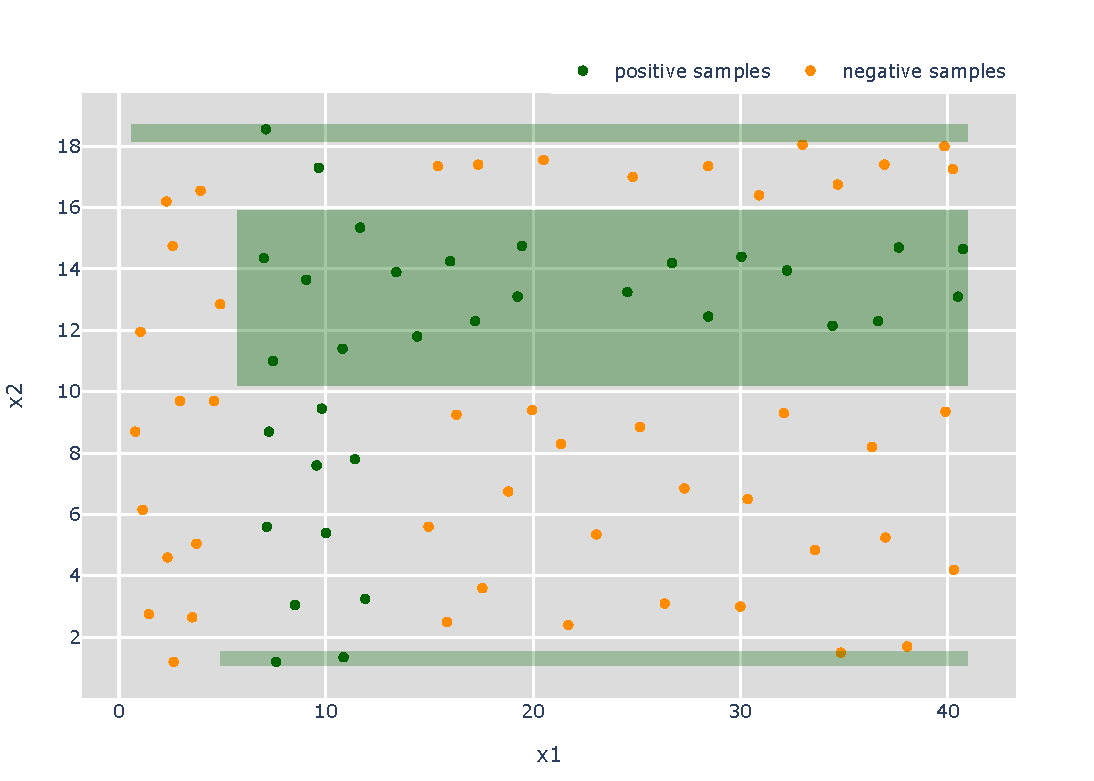
\includegraphics[width=0.85\columnwidth]{figures/cross_1.pdf}
        \caption{\(p = 1\).}
    \end{subfigure}
    \hfill
    \begin{subfigure}{\textwidth}
        \centering
        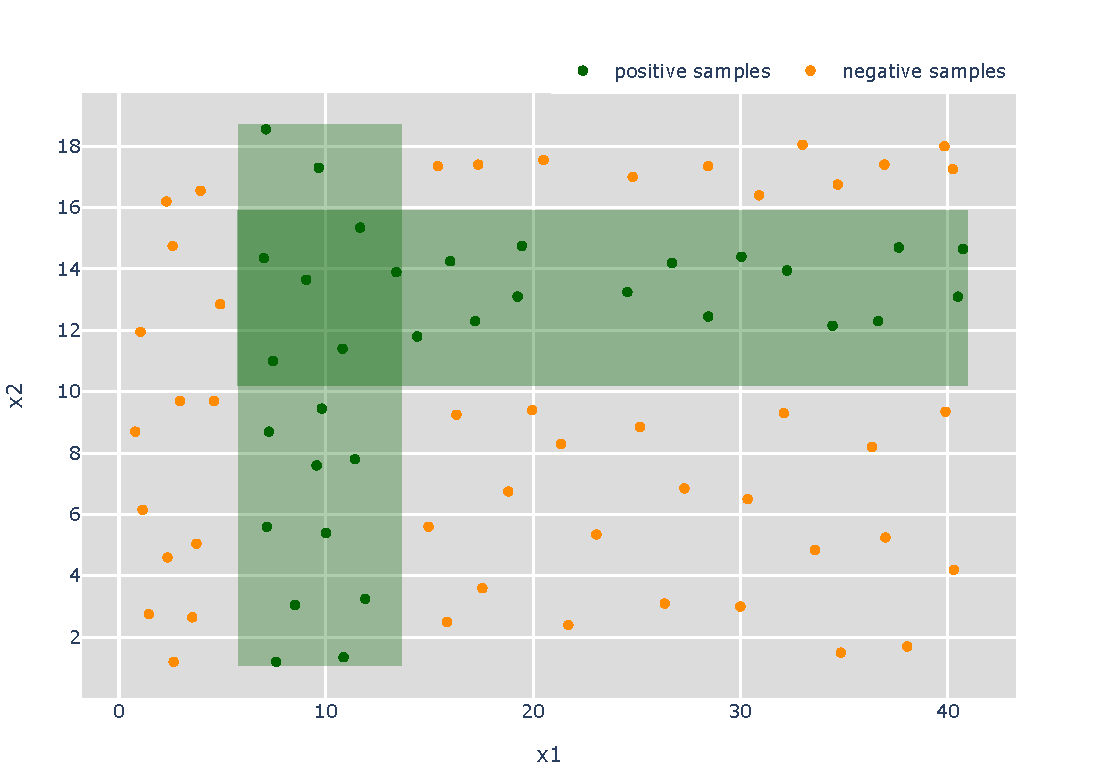
\includegraphics[width=0.85\columnwidth]{figures/cross_1_5.pdf}
        \caption{\(p = 1.5\).}
    \end{subfigure}
    \caption{Classification rule for an artificial data set with two orthogonal decision regions. Both models use a \(minConjSize\) of \(1\).}\label{fig:crossP}
\end{figure}

This can be illustrated using the example of \autoref{fig:crossP}:
Here the algorithm with \(p=1.5\) finds the reasonable decision rule `\texttt{IF (x2 > 10.35 AND x2 < 15.77 AND x1 > 5.95) OR (x1 < 13.42 AND x1 > 6.0) THEN class 1}',
however the algorithm with \(p=1\) finds a far less suitable one.
While they both have the same first conjunction, the more risky algorithm then chooses the ray `x1 < 13.42', which
the other algorithm did not choose.
This is because, without knowing that there is a perfect ray `x1 > 6.0' that can be chosen next,
this ray evaluates to 12 new positive samples to be correctly classified and 14 negative samples to be misclassified.
So even though the situation seems quite obvious for a human observer, rays often decide for
more defensive selections of rays next to the data set's borders, like the SCM with \(p=1\) did here.

When using \(p = \inf\) the SCM always selects the conjunction first, that is guaranteed to cover all positive samples, without considering
the misclassified negative samples at all.
This leads to a \(SCM_{DNF}\) that would always only consist of one single conjunction and
is therefore an unnecessary option to consider in this thesis.

As it is quite complicated to come up with a mathematical formula to compute the penalty parameter \(p\)
that maximizes the classifiers accuracy, I instead focus on balancing the
specificity and the sensitivity of a DNF classifier.
This configuration does in general not maximize the accuracy, yet it ensures that the weaker class has a reasonable accuracy, too. % self driving car and pedestrian

The usefulness of a base classifier, and therefore the possibility that it is chosen, is defined as
\[Q - p \cdot R = \text{`correctly classified negative samples'} - p \cdot \text{`misclassified positive samples'}\]
The parameter \(p\) therefore defines the weight balance between positive and negative samples.
By setting \(p\) as \(\frac{|\text{`neg.\ samples'}|}{|\text{`pos.\ samples'}|}\) this balance is approximately evened out,
as \[\text{`correctly classified neg.\ samples'} - \frac{|\text{`neg.\ samples'}|}{|\text{`pos.\ samples'}|} \cdot \text{`misclassified pos.\ samples'} \approx 0\]
In this way an SCM with approximately the same sensitivity and specificity can be created.
However the formula requires \(sC\) and \(sD\) being high enough and \(minConjSize\) being small enough, so the ratio will not be influenced by these factors.
Moreover the training and the test data's class 1 to class 0 samples ratios need to be round about the same.
This is for example provided when the test data is generated by a cross-validation (see \autoref{sec:evalMethods}).
The formula will later be tested on the `german' data set in \autoref{subsec:german}, as this data set has an especially uneven ratio of classes,
as well as on the gene expression data sets in \autoref{subsec:studySCM}.

%%%%%%%%%%%%%%%%%%%%%%%%%%%%%%%%%%%%%%%%%%%%%%%%%%%%%%%%%%%%%%%%%%%%%%%%%%%%%%%%%%%%%%%%%%%%
\section{Making Use of Ties}\label{sec:ties}

% idea
Often times, when comparing different thresholds, operators or features, the SCM will come across base classifiers that have the exact same score.
Those base classifiers can be considered as `ties'.
~\cite{kestler06} already suggested that `break[ing] ties of equivalent greedy solutions'~\citep[p. 296]{kestler06} may increase the SCM's robustness.
I now want to investigate on this idea in the context of DNF decision rules.

Usually only one of those options is picked and the other one is discarded, however the \(SCM_{DNF}\)
seems like a good framework for actually making use of those ties, as the SCM can
store both base classifiers, complete the conjunction with the first base classifier and then append the second base classifier and its conjunction using a logical-OR.\
Additionally it has to be considered, that there might also be three or more ties at once and new ties might appear
while the SCM is still resolving another tie.

In order to work with ties, some adaptions to the Julia code are needed:
In \texttt{inspect\_\\single\_feature\ (NominalFeature)} and \texttt{find\_border} not only one optimal threshold, but all thresholds,
that share the highest score, need to be returned, as depicted in \autoref{julia:tiesCollect1}.
Similarly, in \texttt{inspect\_single\_feature\ (NumericalFeature)}, if the optimal ray using \(\geq\)
and the optimal ray using \(\leq\) have equal scores, both will be returned (see \autoref{julia:tiesCollect2}).
As \texttt{find\_base\_classifier} compares the base classifiers of the different features and returns the optimum, ties can also occur here
and need to be collected by a procedure like the one in \autoref{julia:tiesCollect3}.
However the main difference is in the \texttt{build\_conjunction} function.
Here all ties from the subfunctions get collected.
One base classifier is then used immediately while the others are returned to \texttt{build\_dnf} together with their
histories, i.e.\ all base classifiers that were selected in this conjunction so far.
There they will then be stored and used as an input parameter for the next \texttt{build\_conjunction} calls.
This is illustrated in \autoref{julia:buildDnfTies}.
In particular \texttt{popfirst!} ensures that always latest found tie is used for the next conjunction.
Whenever \texttt{build\_conjunction} is now called with some preselected base classifiers from a recent tie,
these base classifiers are used as the classifier's preamble and the algorithm continues to extend their conjunction.
However these ties still need to pass the \(minConjSize\) test or otherwise the algorithm is immediately terminated.
This modified \texttt{build\_conjunction} function can be found in \autoref{julia:buildConjTies}, while the old one is depicted in \autoref{julia:buildConj}.

But in fact, the base classifiers are only helpful in very few cases.
For example in the situation of \autoref{fig:tiesA}, when using \(p=1\), there will be the tie between the rays \(x < \alpha\) and \(x < \beta\).
These ties are definitely worth tracking.
The same goes for \autoref{fig:tiesB}, where all four rays \(x < \alpha\), \(x > \alpha\), \(y < \alpha\) and \(y > \alpha\)
have the same usefulness score and can therefore be considered as ties.
Yet, here the selection might already be unlucky: if one for example selects \(x < \alpha\) first, followed by \(y < \alpha\)
to complete the conjunction, the selection of the previous tie \(y < \alpha\) as the first ray for the next conjunction would lead to 
an immediate end of the algorithm with only `\texttt{IF \(x < \alpha\) AND \(y < \alpha\) THEN class 1}' as the classification rule,
without the consideration of the positive samples within \texttt{`\(x > \alpha\) AND \(y > \alpha\)}'.
In the case of the data set depicted in \autoref{fig:tiesC}, using ties is rather counterproductive,
as only one ray is needed, \(x < \alpha\) or \(y > \alpha\).
Therefore it is quite useless to memorize the second ray as well.
Moreover in the situation of \autoref{fig:tiesD}, all four marked rays have the same scores when using a penalty value of 1.
Yet, again luck for the correct order of choosing rays is needed.
If for example \(x < \alpha\) is chosen first, followed by \(x < \beta\), \(x < \gamma\) and finally \(x < \delta\),
the SCM ends up with a pretty bulky classification rule that barely has any significance.

In general it is often the case that there are many ties present, however most of them are comparatively useless and will only make the algorithm terminate.
This is due to the fact that samples that are classified by the current conjunction are removed from the data set before continuing
to resolve the tie situations.
In the scenarios \autoref{fig:tiesB}, \autoref{fig:tiesC}, \autoref{fig:tiesD} and many more this means that the investigation on the tie does usually not at all equal the investigation on the currently optimal ray.
A study about the performance of an SCM that utilizes ties when working on gene expression data can be found in \autoref{subsec:studySCM}.

\begin{figure}
    \centering
    \begin{subfigure}[b]{0.5\textwidth}
        \centering
        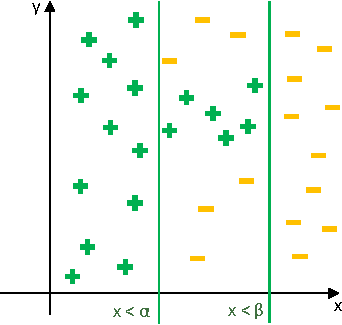
\includegraphics[width=\textwidth]{figures/ties_A.pdf}
        \caption{Situation A.}\label{fig:tiesA}
    \end{subfigure}%
    \begin{subfigure}[b]{0.5\textwidth}
        \centering
        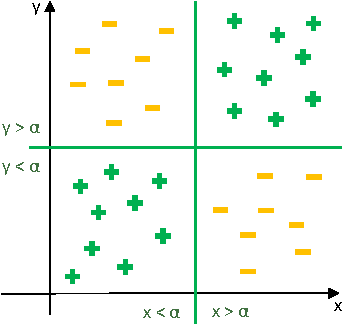
\includegraphics[width=\textwidth]{figures/ties_B.pdf}
        \caption{Situation B.}\label{fig:tiesB}
    \end{subfigure}
    \begin{subfigure}[b]{0.5\textwidth}
        \centering
        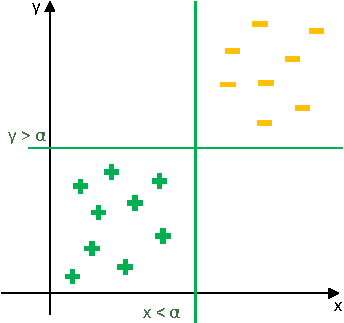
\includegraphics[width=\textwidth]{figures/ties_C.pdf}
        \caption{Situation C.}\label{fig:tiesC}
    \end{subfigure}%
    \begin{subfigure}[b]{0.5\textwidth}
        \centering
        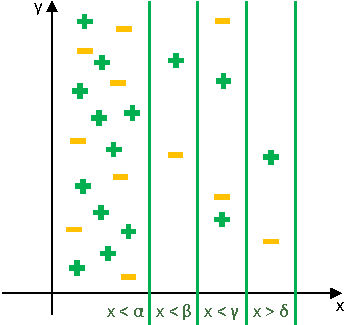
\includegraphics[width=\textwidth]{figures/ties_D.pdf}
        \caption{Situation D.}\label{fig:tiesD}
    \end{subfigure}
    \caption{Scenarios, in which the utilization of ties is more or less useful.}\label{fig:ties}
\end{figure}

I additionally tried an implementation, in which a tie base classifier, that does not fulfill the algorithms requirements
of correctly classifying at least one positive and one negative sample, does not lead to an immediate termination of the algorithm,
but instead the tie is discarded and the algorithm goes on with the next iteration.
However this algorithm led to extremely high execution times, as even on data sets with only a few hundred samples and features
thousands of ties were checked and discarded again, making the algorithm so slow that it is simply not feasible to use on bigger data sets.
\chapter{Identifying and Optimizing Base Classifiers for Various Feature Types}\label{ch:varFeat}

Data sets may have many different kinds of features: besides floating point numbers, integers and Booleans,
they often also contain single characters or whole character strings.
Often times one data set even contains features of different data types.

\begin{figure}[ht]
    \centering
    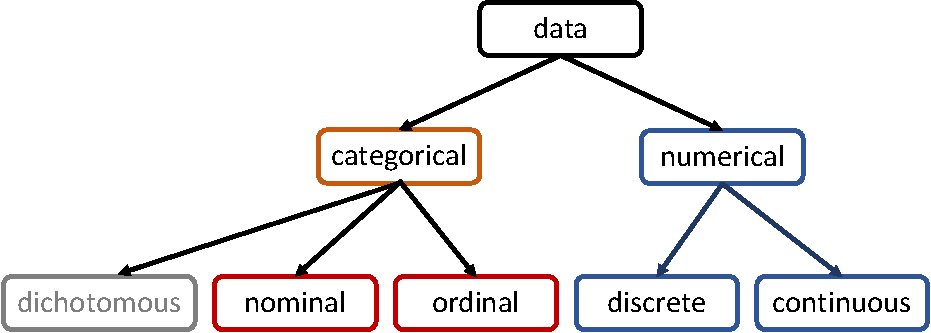
\includegraphics[width=\columnwidth]{figures/data_classes.pdf}
    \caption{Hierarchy of the different data types~\citep{brownlee,dahouda}.}\label{fig:dataClasses}
\end{figure}

% Types of Data
The most common approach is to group data into categorical and numerical types, as seen in \autoref{fig:dataClasses}.
While numerical data is represented in the form of numbers, categorical data is usually represented by character strings.
Continuous variables are real-valued floating point numbers that are defined over uncountable sets of values like \(\mathbb{R}\).
Discrete variables, in contrast, are defined over countable, finite sets of values and are required to have a one-to-one correspondence to \(\mathbb{N}\).
Ordinal variables, like \(\text{size} \in \{\text{S, M, L}\}\), have embedded orderings,
whereas nominal variables, like \(\text{color} \in \{\text{red, green, blue}\}\), do not have such underlying hierarchies.
Moreover dichotomous variables, also known als binary variables, have exactly two distinct values~\citep{brownlee, dahouda}.

% the SCM handling numerical variables
Numerical variables are easy to process for most machine learning algorithms.
In particular, the SCM with data-dependent rays is defined on numerical data and can handle both, continuous and discrete variables, effortlessly.
Due to the natural limitation of features values, caused by the finite amount of samples, every feature dimension is essentially discrete.
This enables the uniform processing of continuos, as well as discrete, variables within the SCM.\

% ML algorithms fail on categorical features
Even though categorical features are very common in real-world problems, 
many machine learning algorithms are not capable of processing raw text as an input for their features~\citep{dahouda,potdar}.
Often times those categorical features first need to be encoded into numerical ones, in order to be processed.
~\cite{dahouda} introduce some very advanced encoding mechanisms, however, such encoding usually still
involves a loss in performance of the classification algorithm,
the need of an increased amount of features, as well as a loss of the data's expressiveness,
and should therefore be avoided.

% the SCM handling nominal and mixed variables
As nominal variables have no embedded ordering and therefore rules like `color >= blue' make no sense,
nominal features cannot simply be transformed into numerical
features and need to be handled in a separate routine.
A dichotomous variable can, and will in this thesis, also be handled as a nominal variable with the small value range of size two.
This has the advantage that is allows the variable to not only be a Boolean, but any kind of binary
value set, like for example \{fast, slow\}.
Therefore the SCM's routine, of looking for the best possible base classifier on each feature, is split into two:
One routine to examine a numerical feature (see \autoref{sec:numerical}) and one to examine a nominal feature (see \autoref{sec:nominal}).

% the SCM handling ordinal variables
The SCM could furthermore handle ordinal variables either like nominal variables, but paired together with an order relation~\citep{dahouda},
or they can be parsed, together with an explicit notation of their underlying order relations, into a discrete variable.
However I decided not to support ordinal variables, as the implementation is quite
unspectacular and I do not want to make the code unnecessarily complex.
Additionally, it is sometimes even beneficial to manually convert ordinal variables into discrete numeric ones,
for example by substituting \texttt{\{child,teenager,senior\}} for \texttt{\{5,15,65\}},
as this gives the user the chance to include semantics that would have been lost otherwise,
like `teenager' being closer to `child', than to `senior'.

The final SCM can now not only deal with floating point numbers and integers by applying a routine for numerical features,
but also handle character strings --- and consequently even Booleans and single characters
as those are parsed into character strings implicitly by the Julia mechanics.
On these raw text features the algorithm then applies a routine for nominal features.
It is moreover by-default possible for this modified SCM to analyze data sets with mixed feature types,
provided that each feature is of one distinct type.
This works, as the SCM with such single threshold base classifiers assesses each feature dimension independently and is therefore
able to handle inconsistent feature types effortlessly~\citep{schmid}.
This enables mixed type rules like `\texttt{IF color = black AND radius >= 2.5 THEN wheel}' that barely any other machine learning algorithm is able
to produce as easily, as the SCM does.

Julia generally recognizes the type of each feature, i.e.\ the data type of the feature's column within the data frame, automatically.
It only needs a little help for parsing strings from CSV files, as displayed in \autoref{julia:loadCsv}.
My SCM then works with the data types `\verb|const NumericalFeature = Union{Vector{Float64}, Vector{Int64}}|'\\
and `\texttt{const NominalFeature = Union\{Vector\{Bool\}, Vector\{String\}\}}'.\\
When examining a feature for high scoring base classifiers, the algorithm now employs multiple dispatch to use one function
on all nominal features and another function on all numerical features.
A data set might for example resemble the one in \autoref{tab:mixed_data}.
The features types were added by Julia automatically, initially it was a plain CSV file.

\begin{table}[ht]
    \centering
    \caption{Data set with mixed feature types.}\label{tab:mixed_data}
    \begin{tabular}{l|lllll}
        Row & x1 & x2 & x3 & x4 & label \\
         & Float64 & Int64 & Bool & String & Int64 \\
        \midrule
        1 & 0.1323 & 15 & false & red & 0 \\
        2 & 0.7046 & 127 & true & blue & 0 \\
        3 & 0.2139 & 9 & false & purple & 1 \\
        4 & 0.5103 & 300 & true & white & 1 \\
        5 & 0.1685 & 111111 & false & green & 0 \\
        6 & 0.699 & 210 & false & orange & 1 \\
        7 & 0.374 & 16 & false & red & 0 \\
        8 & 0.08105 & -50 & false & blue & 0 \\
        9 & 0.7964 & 17 & false & purple & 1 \\
        10 & 0.0954 & -3 & true & purple & 1
    \end{tabular}
\end{table}

%%%%%%%%%%%%%%%%%%%%%%%%%%%%%%%%%%%%%%%%%%%%%%%%%%%%%%%%%%%%%%%%%%%%%%%%%%%%%%%%%%%%%%%%%%%%
\section{Locating Optimal Base Classifiers on Numerical Features}\label{sec:numerical}

To find and evaluate data-dependent rays on a numerical feature the procedure in \autoref{code:numerical} is executed.
Here the SCM first looks for a border to delimit the feature from above, then from below and finally it returns the optimum of both.
This leads to a total number of \(2 \cdot |\text{samples}| \cdot |\text{numerical features}|\) possible rays that need to be evaluated.
However in fact not every sample will have a different value for this feature and therefore
the algorithm's `featureVector' can be reduced by removing all its duplicates.
This reduces the total number of possible rays to only \(2 \cdot |\text{unique sample-feature values}| \cdot |\text{numerical features}|\).

\begin{algorithm}[ht]
    \KwIn{featureVector, labelVector, \(p\)}
    \For{featureValue \(\in\) featureVector}{
        Calculate the usefulness score of the ray `feature \(\leq\) featureValue' using \autoref{julia:calcScore}.
    }
    upperBorder = ray of this loop with the maximum usefulness score \\
    \For{featureValue \(\in\) featureVector}{
        Calculate the usefulness score of the ray `feature \(\geq\) featureValue' using \autoref{julia:calcScore}.
    }
    lowerBorder = ray of this loop with the maximum usefulness score \\
    Return the border with the higher usefulness score.
    \caption{Basic algorithm to determine the optimal ray on a certain numerical feature.}\label{code:numerical}
\end{algorithm}

% Optimization: Clever Score Calculation
This algorithm can be heavily optimized: the result will be the same, yet the execution time can be
decreased from \(\mathcal{O}(|\text{samples}|^2)\) to only \(\mathcal{O}(|\text{samples}|)\),
enabling the SCM to process even huge data sets, such as the gene expressions in \autoref{sec:geneticData}.
Instead of considering the feature value of every sample for the score calculation of a possible threshold,
the optimized algorithm iterates through all samples only once and calculates the current positions's scores based
on the last positions's score, without needing to check every sample in a nested loop.

The algorithm, that is depicted in \autoref{julia:inspectNumerical}, then works as follows:
First all values that the samples have at this feature component are collected, duplicates are removed
and the final vector is sorted from low values to high values.
Each of these possible thresholds then gets assigned two numbers: the number of positive samples that
have this value as its feature component and the number of negative samples that do so.
Afterwards the lower and upper border are again calculated and the optimal border is returned.
Yet, this time an optimized algorithm, illustrated in \autoref{julia:findBorder}, is used.
This new algorithm based on the fact, that Q and R always only change by the number of positive and negative samples that had the
last threshold as their feature value.
As the possible thresholds are ordered from low to high, the optimal lower
border is located first, in order to use the fact that both, Q and R, of the ray `\(x \geq \text{minValue}\)' are always 0,
as every sample is placed within this ray.
The analog fact also applies to the ray `\(x \leq \text{maxValue}\)', which is why the vector
of all possible thresholds is reversed before looking for the optimal upper border later on.

Starting from \(Q=R=0\) for the first threshold, the values of the next threshold can be calculated by
\[Q_{new} = Q_{old} + |\text{`negative samples at the previous threshold'}|\]
\[R_{new} = R_{old} + |\text{`positive samples at the previous threshold'}|\]
For example in the case of \autoref{fig:lowerBorder}, the algorithm starts on the very left
with \(Q=R=0\) and continues to advance to the right with \(Q=0\)  \(R=1\), \(Q=1\) \(R=2\) and so on.
Regarding the upper border on the reversed threshold vector, this also works in the same way.
On the same data, the algorithm this time starts on the very right
with \(Q=R=0\) and then proceeds with \(Q=1\) \(R=0\), \(Q=3\) \(R=0\) and so on (see \autoref{fig:upperBorder}).
A single threshold classifier's score is then, as always, deducted by \(Q - p \cdot S\).

\begin{figure}[ht]
    \centering
    \begin{subfigure}{\textwidth}
        \centering
        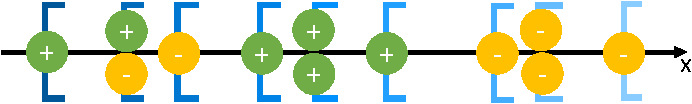
\includegraphics[width=0.85\columnwidth]{figures/lower_border.pdf}
        \caption{Advancing from left to right to evaluate possible lower borders.}\label{fig:lowerBorder}
    \end{subfigure}
    \hfill
    \begin{subfigure}{\textwidth}
        \centering
        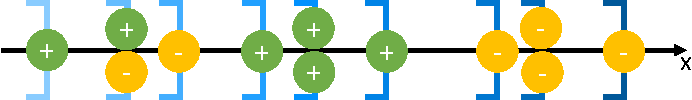
\includegraphics[width=0.85\columnwidth]{figures/upper_border.pdf}
        \caption{Advancing from right to left to evaluate possible upper borders.}\label{fig:upperBorder}
    \end{subfigure}
    \caption{Iteration through a feature vector to locate optimal borders.}\label{fig:borders}
\end{figure}

%%%%%%%%%%%%%%%%%%%%%%%%%%%%%%%%%%%%%%%%%%%%%%%%%%%%%%%%%%%%%%%%%%%%%%%%%%%%%%%%%%%%%%%%%%%%
\subsection{Dealing with the Re-correction of Rays}

% the situation
The SCM is choosing one ray after another and adds them to the conjunction.
However it often also chooses rays that have the same feature-operator combination as a previously selected rule.
This leads to rules like `\texttt{IF x1 < 5 AND x1 < 3}', where the first ray is basically `re-corrected'.
The re-correcting ray will always be tighter than the first one, since the conjunction
algorithm deletes all positive samples outside the chosen rays in every iteration,
making it impossible that rays with thresholds outside those previous conjunctions are selected afterwards.
Moreover re-correcting will never happen on nominal features, as all other threshold regarding this feature
are immediately outside of the conjunction, once a base classifier regarding this feature is chosen.
To illustrate this, the rule `\texttt{IF x2 = blue AND x2 = red}' can be taken into account, that will always evaluate to `false'.

\begin{figure}
    \centering
    \begin{subfigure}{\textwidth}
        \centering
        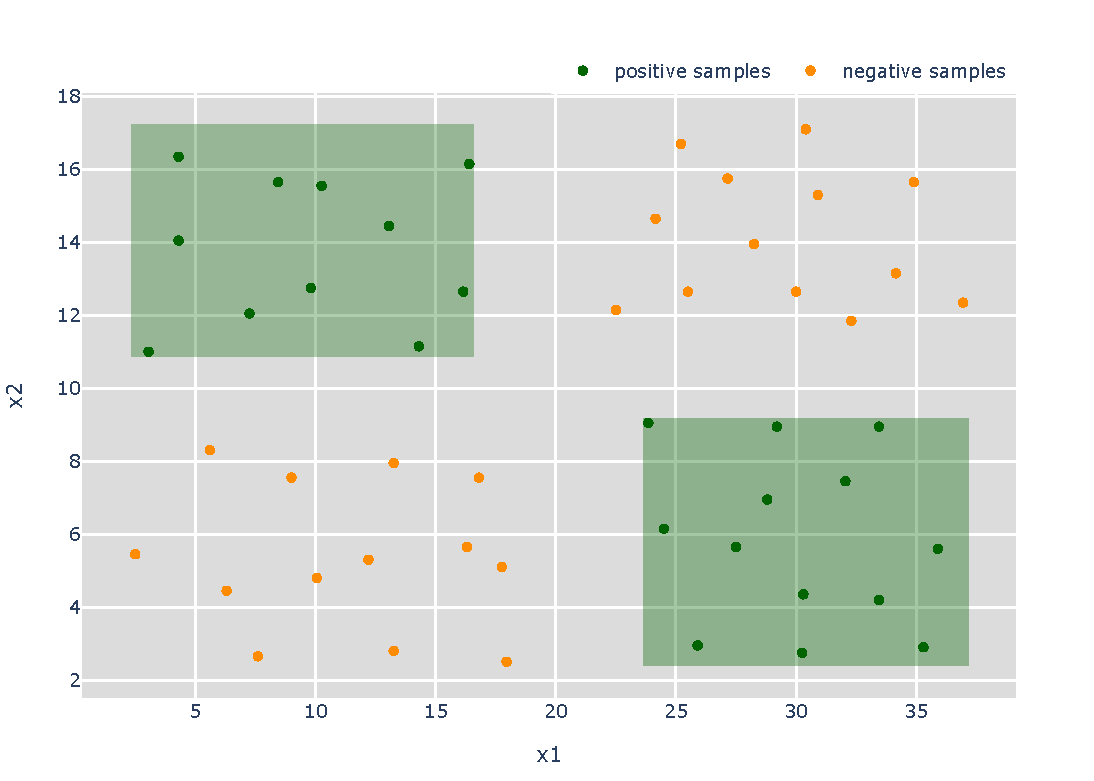
\includegraphics[width=0.85\columnwidth]{figures/two_reg_recorrecting.pdf}
        \caption{Re-correcting allowed.}\label{fig:withRecorr}
    \end{subfigure}
    \hfill
    \begin{subfigure}{\textwidth}
        \centering
        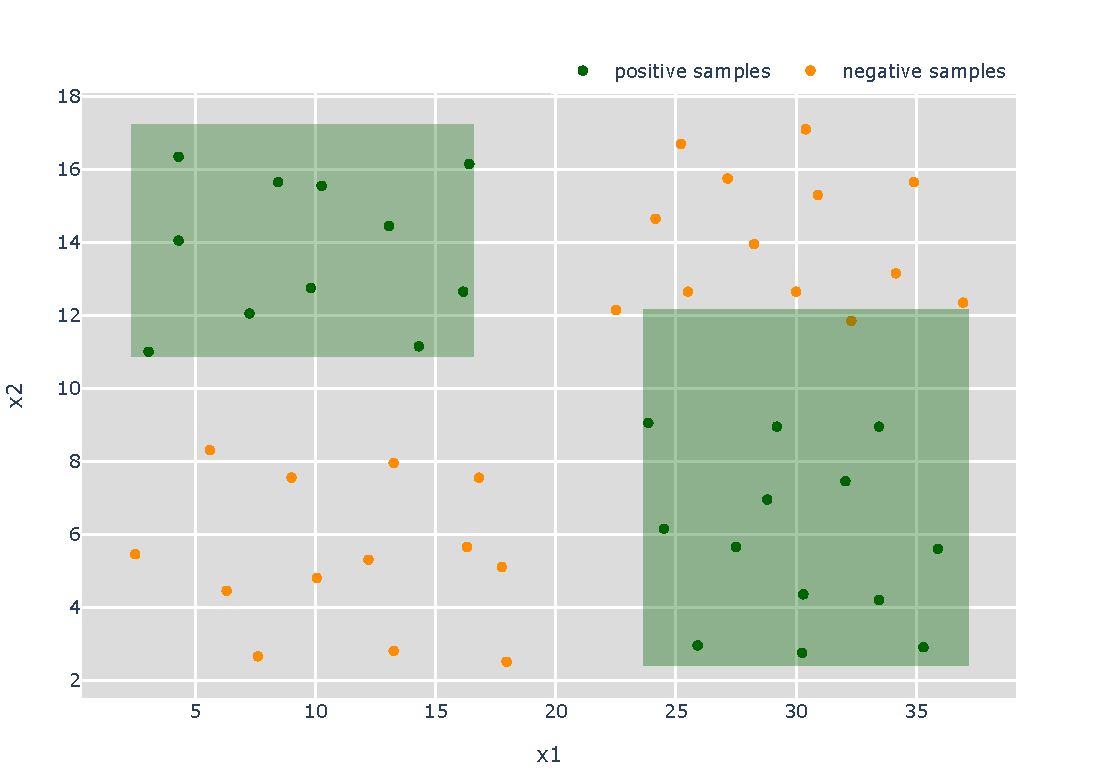
\includegraphics[width=0.85\columnwidth]{figures/two_reg_no_recorrecting.pdf}
        \caption{Re-correcting prevented.}\label{fig:noRecorr}
    \end{subfigure}
    \caption{Classification rule for an artificial data set with two disjunct decision regions.
        In both cases \(p\) is set to 1.2 and \(minConjSize\) to 1.}\label{fig:recorr}
\end{figure}

% how to prevent re-correcting
The process of re-correcting may be prevented by placing the code block of \autoref{julia:preventRecorr} in front of
the usefulness score computation of every ray, to ensure that rays, that would otherwise re-correct
previously chosen rays, will not be selected.
Yet this re-correcting behavior is in general a good thing, as it usually improves the algorithms results,
like in the example of \autoref{fig:recorr}, by reducing the decision region within the rays
to a better size, now that the SCM with data-dependent rays knows the new, more limited, region.
Additionally, as \autoref{tab:geneCompact} illustrates, the chance of actually deciding to re-correct
when working in a big feature space is actually really small.
Yet in order to prohibit the overriding of rays, many parameters need to be parsed down to low-level functions.
So in the common case of having many features and therefore usually not even considering to re-correct, having
the `feature' to prohibit re-correcting, slows down the whole SCM.\

% conclusion
Therefore I allow the SCM to re-correct previously made ray choices and
include the line `\texttt{filter!(r -> r.featureId!=ray.featureId || r.operator!=ray\\.operator, selectedRays)}'
to the end of the \texttt{build\_conjunction} algorithm, to delete the overridden ray.

%%%%%%%%%%%%%%%%%%%%%%%%%%%%%%%%%%%%%%%%%%%%%%%%%%%%%%%%%%%%%%%%%%%%%%%%%%%%%%%%%%%%%%%%%%%%
\subsection{Placing Thresholds Right in between Data Points}

When using a character to store a numerical ray's direction, the direction can be more than just the binary `\(\geq\)' and `<', as suggested by~\cite{kestler11}.
In this chapter so far the operators `\(\leq\)' and `\(\geq\)' were used for rays
and therefore the thresholds were placed directly on positive samples, like in \autoref{fig:thresholdMin}.
However when using `<' and `>', the thresholds will always be placed on negative samples, as in \autoref{fig:thresholdMax}.
A third option, that will be used from now on, is to place a threshold directly in the center
between the two involved data points, like in \autoref{fig:thresholdMiddle}.

\begin{figure}[h]
    \centering
    \begin{subfigure}{\textwidth}
        \centering
        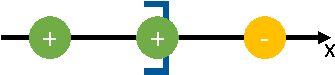
\includegraphics[width=0.5\columnwidth]{figures/threshold_min.pdf}
        \caption{x \(\leq\) 2.}\label{fig:thresholdMin}
    \end{subfigure}
    \hfill
    \begin{subfigure}{\textwidth}
        \centering
        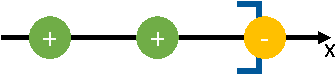
\includegraphics[width=0.5\columnwidth]{figures/threshold_max.pdf}
        \caption{x < 3.}\label{fig:thresholdMax}
    \end{subfigure}
    \hfill
    \begin{subfigure}{\textwidth}
        \centering
        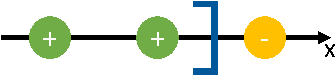
\includegraphics[width=0.5\columnwidth]{figures/threshold_middle.pdf}
        \caption{x < 2.5.}\label{fig:thresholdMiddle}
    \end{subfigure}
    \caption{Possible rays to correctly classify three data points.}\label{fig:variousThresholds}
\end{figure}

This variation can be implemented by extending the method to find a ray on a single numerical feature, depicted in \autoref{julia:inspectNumerical},
with the output of `winnerRay', by an additional functionality that shifts the rays threshold.
So far this threshold is placed directly on the positive sample, with the next sample on the ray's
negative side being a negative one, as a threshold is always placed on the smallest or largest positive sample within an area~\citep{schmid}.
This threshold shifting is generally defined as
\[threshold_{new} = \frac{threshold_{old} + \text{`value of sample next to the ray's negative side'}}{2}\]
and the result will be rounded to two decimals, in order to receive compact thresholds.
However, when trying to process a ray in the form of `\(x \geq \text{minValue}\)' or `\(x \leq \text{maxValue}\)',
there is no more sample on the negative side of the ray and the algorithm, that is furthermore
portrayed in \autoref{julia:thresholdInbetween}, therefore does not modify those rays.

By the definition of~\cite{kestler11} a ray is only considered as data-dependent, if its threshold is directly placed on a sample value.
Therefore the SCM is now per definition dealing with data-independent rays, even though those thresholds do clearly depend on the sample's components.
Additionally the placement of thresholds in between samples comes with the downside that, in case
of integer features, the thresholds might not be integers anymore, but floating-point numbers.
Therefore the rays will not necessarily be located in the feature domain.

However, by placing the threshold in the center of two samples, the ray's margins towards the samples are maximized.
Thus, this version of the SCM is expected to have a lower generalization error~\citep{shawe}.
In data sets like \autoref{fig:tightLooseThr}, the placement of thresholds between samples visibly
does increase the ability of the model to generalize, yet in data sets with many samples, like the gene expressions in \autoref{sec:geneticData},
these improvements are often only marginal, as the large amount of feature values leads to
small gaps between two samples and therefore only small differences between classification
rules with thresholds on and between samples can be identified.

\begin{figure}
    \centering
    \begin{subfigure}{\textwidth}
        \centering
        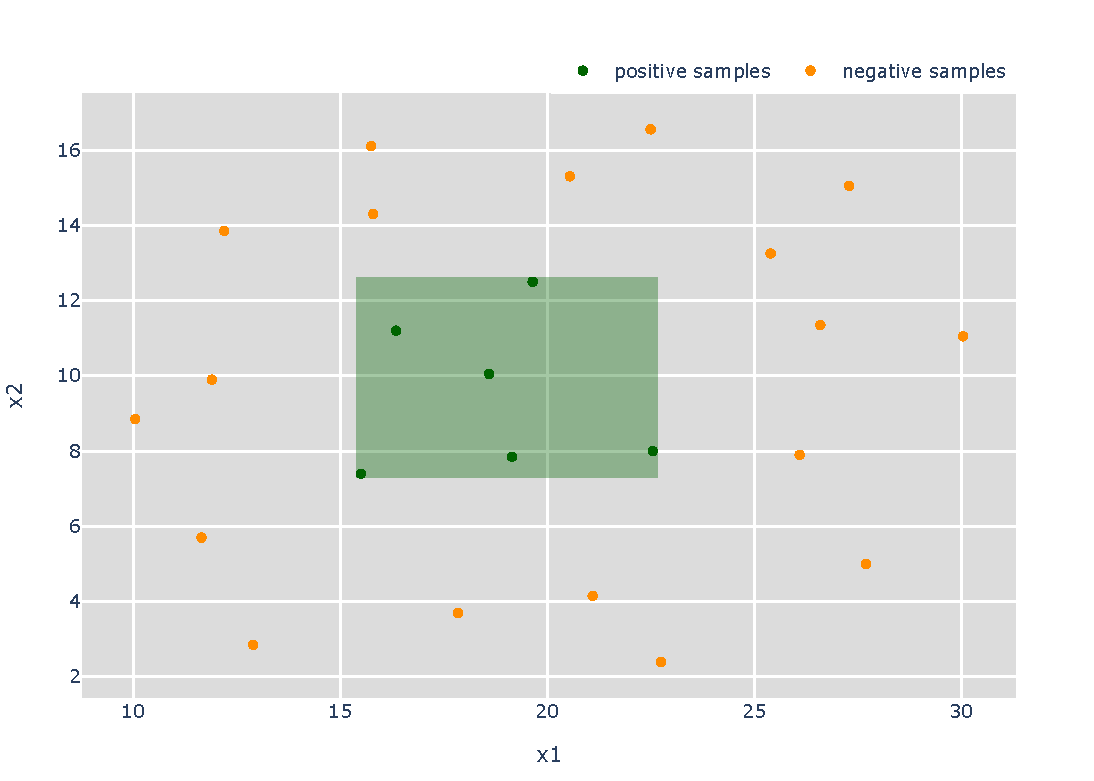
\includegraphics[width=0.85\columnwidth]{figures/one_reg_tight.pdf}
        \caption{Setting tight bounds by placing the thresholds directly on the positive samples.}\label{fig:tight}
    \end{subfigure}
    \hfill
    \begin{subfigure}{\textwidth}
        \centering
        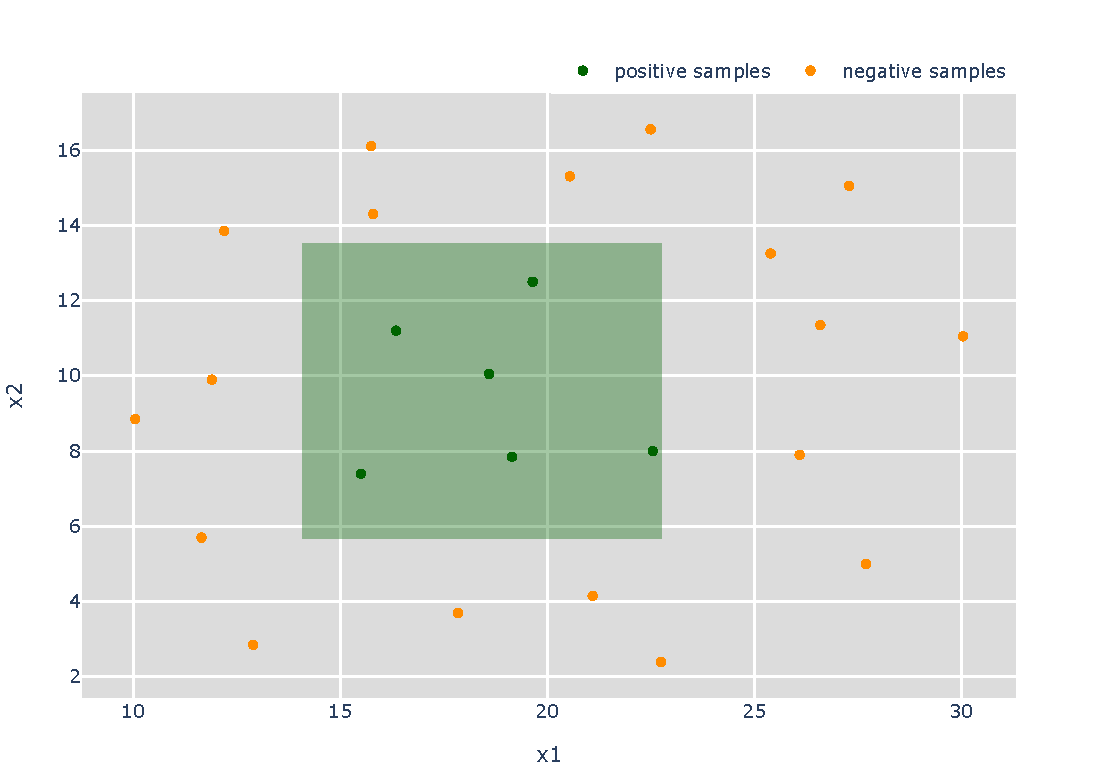
\includegraphics[width=0.85\columnwidth]{figures/one_reg_loose.pdf}
        \caption{Setting loose bounds by placing the thresholds in the centers between positive and negative samples.}\label{fig:loose}
    \end{subfigure}
    \caption{Classification rule for an artificial data set with one central decision regions.
        In both cases \(p\) is set to 3 and \(minConjSize\) to 1.}\label{fig:tightLooseThr}
\end{figure}

After all, as the new thresholds do not classify any of the training samples
differently than the previous version of the algorithm does,
the selection of the next rays is not effected by this design choice.
Therefore the other properties of the classifier, like its number of rays, will in general
be the same as before.

%%%%%%%%%%%%%%%%%%%%%%%%%%%%%%%%%%%%%%%%%%%%%%%%%%%%%%%%%%%%%%%%%%%%%%%%%%%%%%%%%%%%%%%%%%%%
\section{Locating Optimal Base Classifiers on Nominal Features}\label{sec:nominal}

The SCM is moreover extended by a routine that computes the optimal base classifiers on nominal features.
Those can be determined, by executing the algorithm portrayed in \autoref{code:nominal}.
This algorithm simply checks and compares the usefulness scores of classifiers that each limit one feature to one of its sample values.
Analog to the algorithm on nominal features, the duplicates values within the feature vector can be removed to speed up the algorithm.

\begin{algorithm}[ht]
    \KwIn{featureVector, labelVector, \(p\)}
    \For{featureValue \(\in\) featureVector}{
        Calculate the usefulness score of the classifier `feature = featureValue' using \autoref{julia:calcScore}.
    }
    Return the base classifier of this loop with the maximum usefulness score.
    \caption{Basic algorithm to determine the optimal base classifier on a certain nominal feature.}\label{code:nominal}
\end{algorithm}

Two extensions, that are deliberately not implemented, are the `\(\neq\)' and the `\(\in\)' operator.
A `\(\neq\)' operator for nominal features, as in `\texttt{IF x \(\neq\) green THEN class 1}', is not realized in order not to make the algorithm unnecessarily complex.
Features with small value ranges, and especially binary features, do not need a \(\neq\) operator in the first place.
Also, a disjunction of base classifiers on the same feature like \texttt{`x = red OR x = blue OR x = purple'}
is not joined into a set like `\verb|IF x in {red, blue} THEN class 1|', since pure disjunctions like this very rarely, if at all, happen within the \(SCM_{DNF}\).\
Particularly on data sets with many features and an \(sC > 1\), the chance of at least two such
single classifiers of the same feature to appear within the DNF is basically non existent.

% Optimization
Furthermore the complexity of \autoref{code:nominal} is reduced by one dimension, as the last dimension's
Q, R and consequently also its usefulness score, can be deducted from the previous ones:

\[Q_z = |\text{`negative samples'}| - \sum_{i=1}^z Q_i\]
\[R_z = |\text{`negative samples'}| - \sum_{i=1}^z R_i\]

With \(z\) being the last dimension, for example \(z=2\) in the case of a binary feature.
The full implementation, which requires the algorithm from \autoref{julia:calcScore}
to return Q and R additionally to the usefulness score, can be found in \autoref{julia:inspectNominal}.
Testing on the data sets of \autoref{sec:uci} revealed that this new algorithm actually really
improved the SCM's runtime by a bit, as displayed in \autoref{tab:nominalFast}.

\begin{table}[ht]
    \centering
    \caption{Execution times of a \(10 \times 10\) cross-validation using different algorithms for nominal features.}\label{tab:nominalFast}
    \begin{tabular}{lllll}
        \toprule
        & \multicolumn{2}{c}{unoptimized} & \multicolumn{2}{c}{optimized} \\
        data set & execution time & RAM & execution time & RAM \\
        \midrule
        chess & 1.445~s & 4.47~GiB & 1.299~s & 3.82~GiB \\
        german & 0.678~s & 1.43~GiB & 0.672~s & 1.29~GiB \\
        \bottomrule
    \end{tabular}
\end{table}
\chapter{Evaluating the Algorithm on Real-World Data Sets}\label{ch:evaluation}
% !!! to fit on the page the text size in tables may be shorter + use a LOT of abbreviations
% WHAT DOES IT ALL MEAN? - jedes Ergebnis muss tiefgehend (tiefer als die anderen Paper) interpretiert werden!

In this chapter the modified SCM is experimentally evaluated on real-world data sets by conducting \(10 \times 10\) fold cross validations and other analyses,
as introduced in~\autoref{sec:evalMethods}.
Besides investigating on the algorithm's performance, the data sets themselves are also subject to intensive study,
in order to identify their underlying patterns and analyze crucial features and thresholds.
All of the following data sets are binary classification problems.
Their samples have no missing values and are all labeled.

First, two UCI data sets are analyzed in \autoref{sec:uci} to test the SCM on categorical and mixed type features.
Afterwards seven RNA sequencing data sets with high feature dimensions are evaluated in \autoref{sec:geneticData},
to demonstrate the numerical SCM and its applicability in biomedical contexts.
The hyper-parameters \(p\) and \(minConjSize\) will be individually adjusted on each
of these data sets.

\section{Methodology}\label{sec:evalMethods} % / Evaluation Techniques

% need test data
While it can be useful to run the SCM algorithm on all available samples, to see how a classification
rule based on this whole data set would look, the learning algorithm in general needs to be trained and tested on two
independent sample sets, in order for the testing results to be realistic.
However, since all data sets that are analyzed in this thesis only provide training data, but no
independent test data, it is best practice to delegate some of the training samples as test samples~\citep{kestler11}.

% cross validation
To minimize the influence of a more or less favorable selection of the training data subset,
a \(m \times n\) cross-validation, meaning a \(n\)-fold cross-validation, that is done on \(m\) different permutations of the data,
is usually employed for analyzing the performance of an SCM~\citep{muessel, kestler11}.
Within every \(n\)-fold cross-validation, the set of all samples is split into \(n\) groups of approximately equal sizes.
Over the course of the \(m\) iterations, every one of these groups is now once handled as the test group and
otherwise handled as of the training groups, ensuring that there are always \(n-1\) training groups and one test
group in every cycle.
The \(m \times n\) cross-validation finally results in \(m \cdot n\) independent models,
in this case in the form of classification rules.
Those models can then be analyzed as shown in \autoref{subsec:cvOutcomes}.

% cv performance + values for m and n
RAM space is in general no problem for cross-validation computations, as only
the current model, along with very few information about the previously computed models, need to be stored at a time.
However the algorithms runtime is usually crucial, as it is bounded in \(\mathcal{O}(l \cdot m \cdot n)\)
and not really reducible, since all models need to be computed independently.
Here \(l\) denotes the runtime of a single model computation on \(\frac{n-1}{n}\) of the available samples.
When evaluating an SCM, the number of chunks \(m\) and the number of permutations \(n\) are most commonly both set to 10~\citep{kestler11,lausser20}.
This is a good compromise between the high computation times when using high values for \(m\) and \(n\),
and the low utilization rates of samples for training the model, when using low values.

\begin{figure}
    \centering
    \begin{subfigure}{\textwidth}
        \centering
        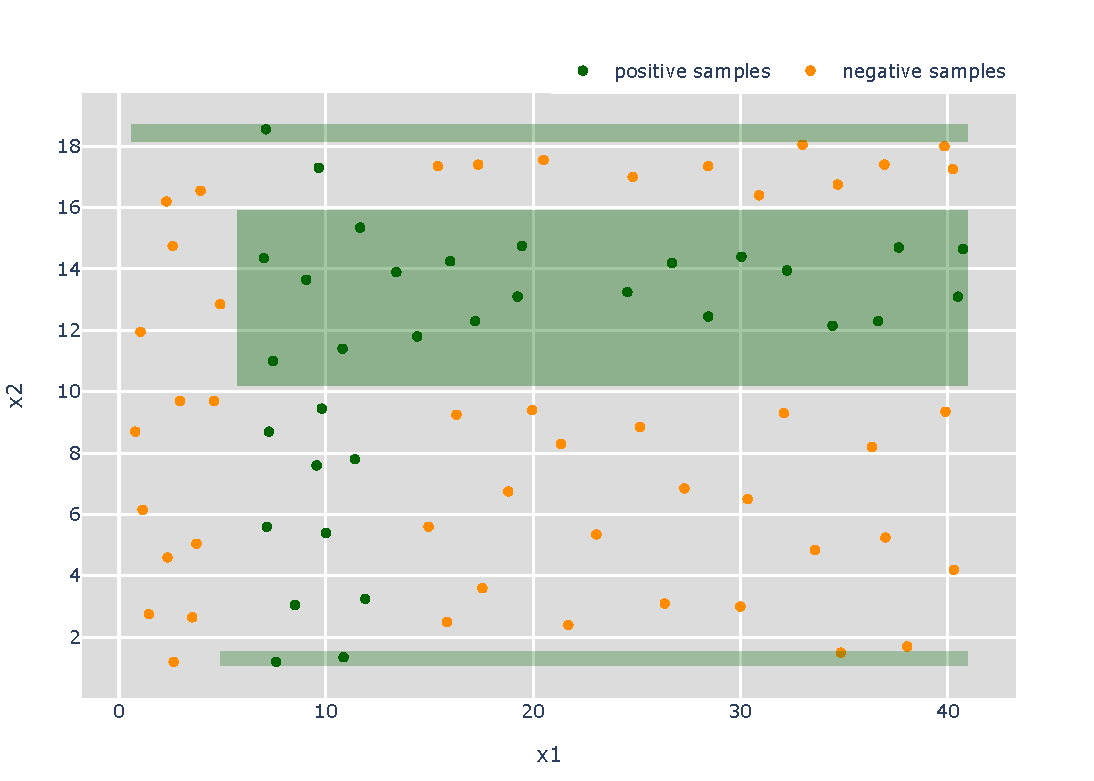
\includegraphics[width=0.85\columnwidth]{figures/cross_1.pdf}
        \caption{Training in the data set with unchanged labels.}
    \end{subfigure}
    \begin{subfigure}{\textwidth}
        \centering
        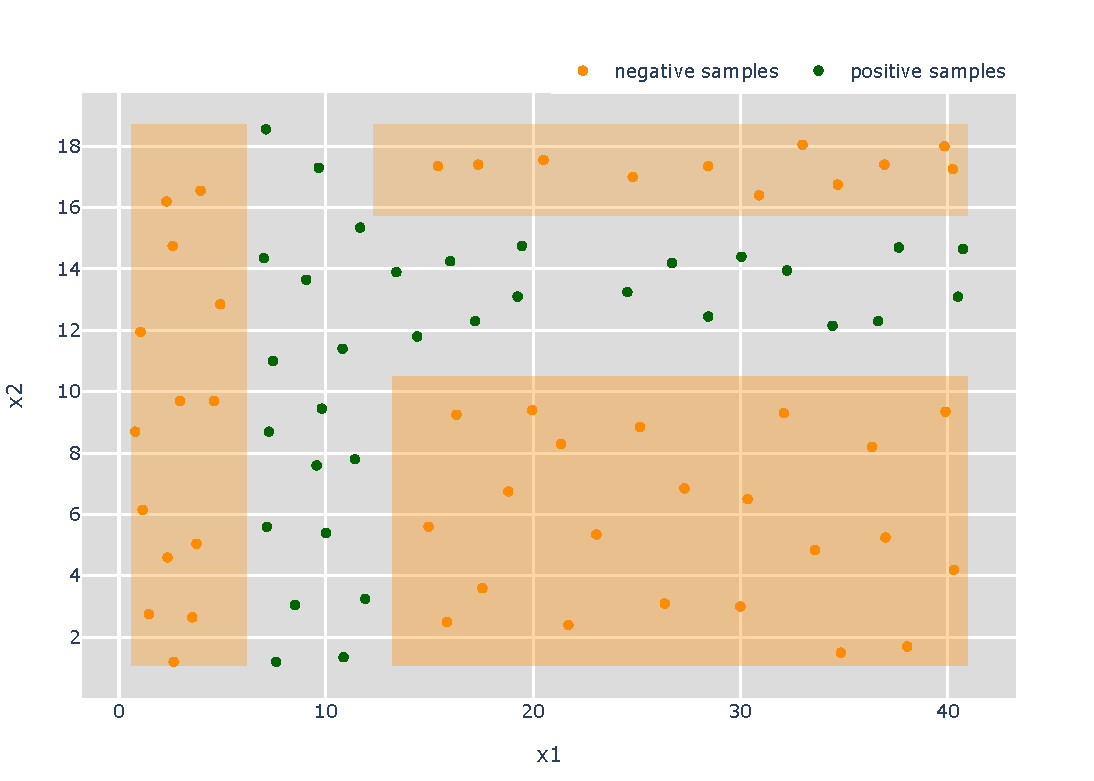
\includegraphics[width=0.85\columnwidth]{figures/cross_1_negated.pdf}
        \caption{Training on the data set with flipped labels.}
    \end{subfigure}
    \caption{Classification rule for an artificial data set with two orthogonal decision regions and its negative.
        Both models use a \(p = minConjSize = 1\).}\label{fig:crossNegative}
\end{figure}

% considering flipped labels
But after all, the \(m \times n\) cross-validation will produce more than 100 models,
as not only the decision rules for classifying samples as class 1, but also those for
classifying them as class 0, are considered, in order to compare the negated and the non-negated DNF and find the best possible models (see \autoref{julia:cv}).
This generally leads to an improved performance of the algorithm, as one context is often more favorable
than the other and therefore produces a better decision rule.
One example for such an improvement is displayed in \autoref{fig:crossNegative}.
In the context of nominal features, computing the decision rules for both classes is especially helpful, as
it often eliminates the need to implement an `\(\neq\)' operator as in `\texttt{IF x5 \(\neq\) green THEN class 1}', by instead using
the negated form `\texttt{IF x5 = green THEN class 0}'.
This negation can be done easily by executing the SCM algorithm twice: once with the unchanged data set \(S\)
and once with \(S\) having flipped labels.
Additionally it is important to set the hyper-parameter \(p\) as \(\sfrac{1}{p}\) and
switch the resulting sensitivity and specificity, when working with flipped labels,
in order to obtain the correct result for a class 0 classification.
After all, the process of finding the optimal model, or even models, can be quite complex, as there are multiple
objectives that the model should fulfill to the highest possible degree-
Yet \autoref{subsec:pareto} presents a highly efficient method to help with this selection.

%%%%%%%%%%%%%%%%%%%%%%%%%%%%%%%%%%%%%%%%%%%%%%%%%%%%%%%%%%%%%%%%%%%%%%%%%%%%%%%%%%%%%%%%%%%%
\subsection{Multi-Objective Model Selection Using Pareto Fronts}\label{subsec:pareto}

Whenever one needs to select a model that optimizes multiple different, often times even opposing, criteria, trade-offs are needed.
The SCM is especially known for the opposing objectives of its classification rules, as they
have to be accurate and compact at the same time.
Therefore a good strategy, to decide for a `good' classifier over a `bad' classifier, is strongly needed.
Traditionally those concurrent goals are assigned fixed weights, so the algorithm can form them into a
hierarchy and find the optimal model for this prioritization of goals, for example by using weighted sums~\citep{muessel}.
Yet, this mechanism has a very unflexible implementation and the weights need to be set in advance.

Another possibility is to use the approach of~\cite{muessel} of selecting all models which are pareto-optimal.
The algorithm works without any fixed weight relation of its objectives and allows all objectives to be treated separately.
A classifier \(b={b_1, b_2, \ldots}\) is pareto-optimal, if no classifier exists that dominates \(b\).
A classifier \(a={a_1, a_2, \ldots}\) would dominate \(b\), if and only if \(\forall i: a_i \geq b_i \land \exists j: a_i \ge b_i\).
In other words, \(b\) is pareto-optional, if and only if there is no other classifier that performs better than \(b\) in
all objectives (\(\nexists a: \forall i: a_i \geq b_i \land \exists j: a_i \ge b_i\))~\citep{muessel}.
This also means that two models with the same values regarding all goals, will always both be selected,
as long as they are not dominated by other models.
The user can then inspect all pareto optimal models and may, but does not have to, select one distinct winner by 
applying an implicit or explicit prioritization function to the objectives~\citep{muessel}.

In case of the SCM, the goal is to choose the best classification rule, regarding both performance aspects, like accuracy,
sensitivity and specificity, as well as compactness, with objectives like a minimizing the number of features and base classifiers.
In order not to make the process unnecessarily complex, I decided to choose only two of those metrics for my studies:
the accuracy, as the most comprehensive measure to describe a models performance, and the number
of features that are used in the decision rule, since the number of base classifiers is already pretty determined by \(sC\) and \(sD\).
Also the number of base classifiers might be subject to further minimization, while the number of features is certainly not.
This pareto front approach (see \autoref{julia:paretoFront}) is now used to determine
whether the model using flipped or un-flipped labels is better, or even both are interesting for
further investigation.

%%%%%%%%%%%%%%%%%%%%%%%%%%%%%%%%%%%%%%%%%%%%%%%%%%%%%%%%%%%%%%%%%%%%%%%%%%%%%%%%%%%%%%%%%%%%
\subsection{Analyzing the Insights Provided by Cross-Validation}\label{subsec:cvOutcomes}

In addition, pareto fronts can also be applied to the 100 or more models, that are the outcome of the
\(10 \times 10\) cross-validation, to filter out the most promising models.
However, one has to keep in mind, that all performance values, like the model's accuracy,
are only subject to \(\sfrac{1}{m} = \sfrac{1}{10}\) of all samples.
As the data sets that are discussed in this paper only contain a few dozen to a few hounded
samples, this share of test samples is so small, that the randomness and luck of
the cross-validation's chunk selection may heavily influence the results.
This leads to the fact that the pareto-optimal models here were actually only pareto-optimal on
a small fraction of the samples, yet cannot be tested on the other ones, as those samples were already used for training.
As a consequence, the set of pareto-optimal models has to be analyzed with high caution,
as the models from different cross-validation cycles are not really comparable to each other.

Therefore the focus is now shifted from working with optimums, to using the plot of the pareto fronts
for analyzing the scattering of the models in the two dimensional space of accuracy and complexity.
Relevant insights like the minimum accuracy of all models or the maximum number of features can be obtained easily here.
Also the percentage of models with accuracies above or below the accuracy baseline can be considered.
This baseline is defined as the fraction of samples in the largest class, to the total amount of samples.
A machine learning algorithm will always achieve an accuracy on the baseline, by simply classifying every sample to the larger class.
In case of heavily uneven classes, the algorithm then might even have a seemingly good accuracy,
however per definition it only learned something valuable, if it is able to outperform the baseline on unseen test data.
However one needs to keep in mind, that this two dimensional plot is constructed in such a way,
that one point in the space may stand for only one or a whole set of models.
Therefore the true distributions of the models cannot be derived from the plots and additional tools to analyze averages are needed.

% Averages
Additionally measurements of the mean characteristics of the models, like the average number of features,
base classifiers or conjunctions per rule, as well as the average accuracy, specificity and sensitivity can be very helpful for certain analysis.
Those values may usually be considered without precautions, as the influences of randomness are evened out by working with medians.
The average accuracy furthermore equals \(1 - \text{cross-validation error}\), where the
cross validation error estimates the generalization error~\citep{muessel}.
To put the number of features, that are used within a classifier, into a context,
the feature compression rate \(1-\frac{|\text{`features in rule'}|}{|\text{`all features'}|}\) might be helpful.
It can be interpreted as the percentage of features that can be reduced by using this
classifier, instead of dealing with the original data set.
Most of the results, including those means, are rounded to two or three decimal digits.
However, this is always done carefully in such a way, that it does not effect the results's interpretations, but only improves the readability a bit.

Another way to represent averages is by using histograms that display what percentage of models share a certain characteristic.
A histogram about the most used features showcases important information about the importance of each feature,
while histograms about the most used base classifiers, both, for base classifiers that contribute to a classification
of the sample as class 0 and as class 1, reveal the main structures within the class distribution.
This separate study of class 0 and class 1 base classifiers is needed, as they have opposing objectives.
In order to make those histograms as informative as possible without flooding the viewer with useless
information, only those base classifiers and features are displayed, that occur in at least 20\% of all
models and can therefore be considered as common.
\section{On the Use of Categorical and Mixed-Type Features: Analyzing UCI Data}\label{sec:uci}

The following two data sets were obtained from the UCI machine learning repository~\citep{uci}.
Thanks to A. Shapiro, R. Holte and P. Clark for providing the `Chess (King-Rook vs. King-Pawn)' data set of \autoref{subsec:chess},
and to H. Hofmann for providing the `Statlog (German Credit Data)' data set of \autoref{subsec:german}.

%%%%%%%%%%%%%%%%%%%%%%%%%%%%%%%%%%%%%%%%%%%%%%%%%%%%%%%%%%%%%%%%%%%%%%%%%%%%%%%%%%%%%%%%%%%%
\subsection{Chess Data Set --- Illustrating the Use of Categorical Features}\label{subsec:chess}

This data set contains 3196 different board configurations that each describe a starting situation
of the chess endgame `King-Rook versus King-Pawn', in which white has only their
king and pawn left and black has only their king and rook left.
Furthermore it is specified that the white pawn is placed on a7 and white has to make the next move~\citep{shapiro}.
Each of the samples is now the description of one of these scenarios.
In 1669 of the scenarios white is able to win (class 1), the remaining 1527 board configurations will end in a
tie or black will win (class 0).

The 36 nominal raw-text features are statements about the current situation of the game.
These statements are, for example, whether the black king is in the black rook's way (`bklbk'),
or whether the white king is on an edge of the chess board, but not on a8 (`cntxt').
Most of them take the value true (t) or false (f) for each sample, however there are also features with
a more complex behavior like `katri', that states whether the black (b) king, the white (w) king or no (n) king
is in control of the intersect point.
The listing and explanation of all the features can be found in~\cite{shapiro}.

The data set was created by~\cite{shapiro} by generating all possible chess board configurations of a King-Rook versus King-Pawn
endgame and sorting them by a set of characteristics using advanced search algorithms and only considering legal moves.
The main goal is now to find out what characteristics are important to have at the beginning of such
an endgame, in order for the white player to win the game.
The modified SCM is perfect for this task, as it can easily handle the nominal features.

% Performing the algorithm and results

When training the \(SCM_{DNF}\) on all data, it creates the classifier `\texttt{IF (bxqsq=f AND wknck=f AND wkna8=f AND hdchk=f AND spcop=f) OR (rimmx=t) THEN\\won}'.
This corresponds with the feature and base classifier histograms of a cross-validation, as illustrated in \autoref{fig:histChessF}, \autoref{fig:histChessR0} and \autoref{fig:histChessR1}.
In conclusion, and using the interpretations of~\cite{shapiro}, my \(SCM_{DNF}\) classifies the following characteristics
as the essential advantages for the white player to win:

\begin{description}
    \item[rimmx = t:] White can capture the black rook immediately.
    \item[bxqsq = f:] Black does not control a8.
    \item[wknck = f:] The white king is not in check.
    \item[wkna8 = f:] The white king is not in a8.
    \item[hdchk = f:] There is no hidden check. A hidden check would for example happen if the white pawn is on a7, the white king on a5, the black king on a3 and the black rook on a1.
    \item[spcop = f:] There is no special opposition pattern, like white pawn on a7, white king on b8, black king on d7 and black rook on d2, present.
\end{description}

In the studies of~\cite{shapiro} using decision trees, he also came to the conclusion that rimmx and bxqsq are among the most important features.
In many experiments he additionally observed the importance of wknck, wkna8, hdchk and spcop.
However he also notices that the latter features are not really efficient on their own, but shall be used in combination with other:
In the context of decision trees he uses them in subtrees, while I use them as follow-up clauses within a conjunction.

\begin{figure}[H]
    \centering
    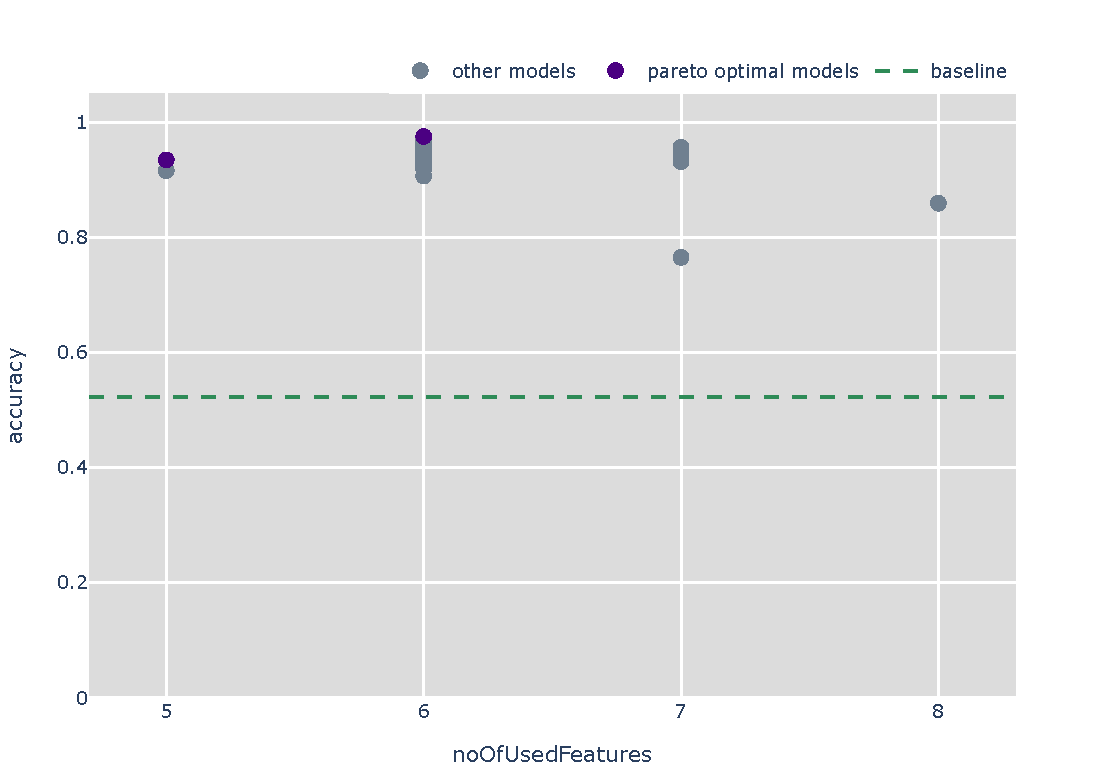
\includegraphics[width=0.85\columnwidth]{figures/chess/paretoFront.pdf}
    \caption{Accuracy-compactness plot for the cross-validation folds of the `chess' data set.}\label{fig:paretoChess}
\end{figure}

With this data set \(p = minConjSize = 1\) was directly usable in order to
obtain good results: in the \(10 \times 10\) cross-validation the \(SCM_{DNF}\) reached a sensitivity of 0.971, a specificity of 0.913
as well as an overall accuracy of 0.943 and therefore a generalization error of only 0.057.
Moreover all 100 models of the cross-validation are located above the baseline (see \autoref{fig:paretoChess}).
In contrast, the \(SCM_{conj}\) only scored an accuracy of 0.809 on the same conditions.
By only using an average of 6.06 features distributed in 2.137 conjunctions per rule, the \(SCM_{DNF}\) is still able to achieve
a good feature compression rate of 83.2\%.

%%%%%%%%%%%%%%%%%%%%%%%%%%%%%%%%%%%%%%%%%%%%%%%%%%%%%%%%%%%%%%%%%%%%%%%%%%%%%%%%%%%%%%%%%%%%
\subsection{German Credit Data --- Illustrating the Use of Mixed-Type Features}\label{subsec:german}

This data set from the Statlog Project contains the data of 1000 applications for a credit in Germany.
700 of these applicants are to be considered as `good' (class 1), the other 300 as `bad' (class 0).
The aim is now to find a rule to classify a new applicant as a good or a bad candidates for a loan, based on their feature values.

As I used the original version of the data set by H. Hofmann, 7 of the 20 features are numerical, like the applicant's age, and 13 are categorical, like purpose of the credit.
Of the categorical features in turn, six are nominal, two binary and therefore handled as nominal and five could be
interpreted as both, ordinal or nominal, so they are treated as nominal.
However, it would certainly be interesting to try and interpret them as ordinal variables in future research.
Additionally the data set is modified by replacing the feature values codes like `A41' with the corresponding real feature values like `car (used)'
from the data set's documentation, so the SCM can produce even more interpretable rules.

The cost matrix, that comes with the data set, implies that the chance of a false positive should be five times lower than the chance of a false negative.
As the chance of a false positive describes the chance that a class 0 samples is classified as class 1, it can be quantified as \(1 - specificity\)
and analog the chance of a false negative equals \(1 - sensitivity\), leading to the requirement of
\[\frac{1-\text{specificity}}{1-\text{sensitivity}} = \frac{1}{5}\]

% Performing the algorithm and results

First of all, different values for \(p\) were tested and the results documented them in \autoref{tab:germanP}.
Here, \(p = \sfrac{3}{7} = \frac{|\text{`negative samples'}|}{|\text{`positive samples'}|}\) was also evaluated, as suggested in \autoref{sec:adjustingParam},
which indeed creates a classifier with a very even sensitivity to specificity ratio.
\(p\) was then gradually decreased until it reached 0.25, at which point the chance of a false negative was
approximately five times higher than the chance of a false positive, fulfilling the data set's requirement.
However, because the data set's classes are very unbalanced, the classifier now only has an accuracy of 0.672,
making it in general even less performant than the trivial classifier `\texttt{IF * THEN good}' with an accuracy of 0.7.

\begin{table}[ht]
    \centering
    \caption{Trying different values for the hyper-parameter \(p\) on the `german' data set.}\label{tab:germanP}
    \begin{tabular}{lllllll}
        \toprule
        \(p\) & acc. \(SCM_{conj}\) & acc. \(SCM_{DNF}\) & |used conj.| & sens. & spec. & \(\frac{1-spec.}{1-sens.}\) \\
        \midrule
        1 & 0.705 & 0.725 & 5.94 & 0.971 & 0.15 & 29.3 \\
        \(\sfrac{4}{7}\) & 0.677 & 0.722 & 9.095 & 0.786 & 0.575 & 1.98 \\
        \(\sfrac{3}{7}\) & 0.669 & 0.672 & 8.545 & 0.667 & 0.698 & \textbf{0.9} \\
        \(\sfrac{2}{7}\) & 0.546 & 0.594 & 8.348 & 0.481 & 0.86 & 0.27 \\
        0.25 & 0.523 & 0.569 & 7.262 & 0.437 & 0.879 & \textbf{0.21} \\
        \bottomrule
    \end{tabular}
\end{table}

The high amounts of used conjunctions per disjunction, depicted in \autoref{tab:germanP},
furthermore indicates that the use of a DNF is indeed helpful for this data set.
Yet it comes with the big trade-off that it increases the size, and therefore the complexity, of the classifier drastically.
This can however be counteracted by increasing the \(minConjSize\).
For \(p=0.25\) the \(SCM_{DNF}\) with \(minConjSize=3\) still has as an accuracy of 0.557
while decreasing the average number of used base classifiers from 18.48 to 11.53 and the number of used conjunctions down to an average of 3.677.

When using the final parameter set of \(p=0.25\) and \(minConjSize = 3\), the resulting
model prefers to give a small credit with a small duration to middle aged people, without
any other installment plans or checking accounts, as portrayed in \autoref{fig:histGermanF} and \autoref{fig:histGermanR1}.
This tendency is also confirmed by the average pareto optimal classifier being
`\texttt{IF (status of existing checking account = no checking account AND\\other installment plans = none
AND age > 22.5 AND credit amount\\< 9504.0 AND age < 66.5) OR (duration in months < 8.5 AND age >\\25.0 AND credit amount < 3015.5)
OR (credit amount < 421.0) THEN good}'.
Additionally \autoref{fig:histGermanR0} provides the insight that 
over 80\% of the classifiers, classify foreign workers to be generally ineligible for a credit.
This is quite shocking, as the data set is only from 1994 and therefore not overly out-of-date.
\section{Analyzing High-Dimensional Gene Expression Profiles}\label{sec:geneticData}

% Cells, DNA and RNA Stuff -> Dogma etc
The human genome, i.e.\ the entirety of genetic information that is stored in the form of 23 chromosome
pairs within every cell's nucleus, consists of about three billion base pairs of nucleic acids~\citep{venter}.
These base pairs are encoded in 20,000 to 25,000 genes that are defined as sections of the deoxyribonucleic acid (DNA).

In order to produce proteins, the genetic information of the DNA is first duplicated, then transcribed
into ribonucleic acid (RNA), more precisely into messenger RNA (mRNA), and subsequently translated into proteins, where it then defines
the protein's characteristics~\citep{crick, koonin}.
The central dogma of molecular biology by~\cite{crick} states that this process, also known as protein biosynthesis, cannot be reversed.
Therefore genetic information is `trapped' in the form of a protein's amino acids, once it is successfully
translated, without the chance of being re-translated into nucleic acids ever again~\citep{crick, koonin}.

While the genes in DNA consist of intron and extron sections, when transcribing, only the exons are kept
and then joined into one long RNA sequence in a process called `splicing'~\citep{wang10}.
The entirety of RNA molecules is then called transcriptome, as it is the ensemble of all RNA transcripts~\citep{malone, venter}.
These transcriptomes are dynamic, in contrast to the static genome~\citep{marguerat}
and provide valuable data on gene expressions, i.e.\ on the genetic and epigenetic characteristics of the cell~\citep{wang09, jones}.

% Genetics and Epigenetics
While the study of genetics addresses the inherited sequence of genes in the genome, epigenetics
focus on the extent, to what the individual genes are activated or deactivated within a specific cell~\citep{jones,jaenisch}.
These distinct gene expressions are influenced by the environment and are
also partially heritable, even though no DNA mutation is involved~\citep{jaenisch}.
A human has an explicit genome that is usually the same in every cell,
whereas the epigenome is in general different for distinct cell types, like liver and pancreas cells,
leading to cell types with different characteristics and functions.

% Cancer research questions -> Why do I want to analyze gene expressions?
Both, genetic and epigenetic, abnormalities are responsible for cancer development at all stages~\citep{jones, jaenisch}. % -> modified gene expressions
One of the main goals of medical oncology is therefore to discover novel genes that are differentially expressed by cancerous and benign cells~\citep{guo13},
or even by different subtypes of cancer.
This can be done by profiling the cell's gene expressions and measuring the differences in gene expression levels between sample classes.
The striking genes potentially produce tumor promoting or suppressing proteins and could therefore be possible starting points for improved cancer treatments.

In the following sections the modified SCM algorithm with data-dependent rays as 
base classifiers is used within a \(10 \times 10\) cross-validation to execute such an analysis on some
extremely high dimensional gene expression data sets, in order to detect compact classification
rules and therefore identify small sets of significant genes.

%%%%%%%%%%%%%%%%%%%%%%%%%%%%%%%%%%%%%%%%%%%%%%%%%%%%%%%%%%%%%%%%%%%%%%%%%%%%%%%%%%%%%%%%%%%%

\subsection{Methods to Quantify, Analyze and Compare Gene Expressions}

% How to analyze gene expressions?
To conduct quantitative analysis of gene expressions, the transcriptome needs to be characterized
by measuring the concentrations of all transcripts that are present at the given time.
This is usually done either by applying microarrays or RNA sequencing, also known as `RNA-seq',
the two most popular high-throughput technologies for gene expression profiling~\citep{li09,guo13}.
Both methods usually result in very similar outcomes~\citep{guo13}, however the two approaches
still have some differences.

% Microarrays and their problems
Microarrays, introduced in~\cite{schena}, are one of the first approaches for the analysis of transcriptomes~\citep{malone}.
Here RNA probes are extracted from samples of two different classes, like benign and cancerous cells, and reverse transcribed into complementary DNA (cDNA).
These cDNAs are then labeled using fluorescent dyes, placed on microarray chips and scanned~\citep{malone}.
A position on the chip will now become discolored, if the gene of this spot is expressed in one of the samples.
This allows comparisons of the expression of each gene in both sample classes.

This technology was especially popular till the 2010s~\citep{guo13} and well established for a long period of time,
leading to a lot of existing research and well assessed standards~\citep{malone}.
However with the introduction of RNA-seq by~\cite{wang09} and the increasing availability
of extremely high-throughput methods to process genetic data, microarrays lost a lot of their popularity~\citep{malone, li09}.

% RNA-seq
RNA-seq accurately estimates gene expression levels by utilizing next-generation sequencing (NGS)~\citep{guo13}.
There are different sequencers available. In the following I will focus in the `Illumina' sequencing protocol of~\cite{wang09}.
To prepare the sequencing library, an extracted RNA probe is broken down into small fragments of about 200 to 300 base pairs each,
which are then re-transcribed into cDNA~\citep{marguerat, wang09}.
These fragments are called `reads'.
The short sequence reads can now be aligned with the reference genome of a sample~\citep{li09}.
Thanks to NGS and its parallel processing, this sequencing process has a very high-throughput~\citep{franchis}.
Yet, reads do not have a 100\% accuracy rate and small errors in mapping happen regularly.
The number of reads that are mapped to a certain gene,also known as the `raw count' of a gene~\citep{li11}, now
estimates the gene expression level of the according gene in the sample~\citep{marguerat, wang09}.

% Normalizations for RNA-seq data
These raw counts may however vary from gene to gene and from sample to sample, as
samples and reads may be of different qualities, depths and lengths~\citep{li11, zhao, guo13}.
In order to ensure the comparability of various sample's gene expressions, these factors of irregularity
need to be offset to the highest possible extent.
This process of normalization then enables the actual estimated quantification of the gene expression levels~\citep{zhao}.

% RSEM
One possibility to estimate gene expression levels, is to use the RNA-seq by expectation maximization (RSEM) software library by~\cite{li11}.
This framework computes an accurate quantification of transcripts even for use cases without a reference genome.
In an RNA-seq reads may map to multiple positions in the reference genome,
usually to isoforms, i.e.\ slightly different versions of the same gene, or splicing junctions~\citep{li09}.
This problem is often solved by simply discarding and reads that have such multiple mappings,
however RSEM instead uses an expectation maximization algorithm that estimates the
true origin of a multi-read expression~\citep{li11}.

% TPM, FPKM, RPKM
The RSEM algorithm then usually returns the resulting expected counts in a transcripts per million (TPM) normalization,
meaning that the counts are first divided by the gene's length in kilobit and subsequently
by the total number of reads that are mapped to this sample \(\times 10^{-6}\)~\citep{zhao, li11}.
This ensures an even scaling of the estimated counts, regarding the gene length, as well as the sequencing depth, and
therefore offsets the transcript's abundances.
Other popular normalizations for RNA-seq data like reads per kilobase million (RPKM) and fragments per kilobase million (FPKM) are not supported by the RSEM library~\citep{li11}.
Those approaches are based on the same two normalization steps as TPM, however this time in a reversed order.
More information on them can be found in~\cite{zhao}.

% final comparison microarray and RNA-seq
Until today an analysis by microarrays is cheaper to realize than one by RNA-seq,
as a huge amount of genes can be processed simultaneously
and even multiple RNA probes can be examined on the same chip~\citep{guo13}.
Additionally the resulting data of a microarray analysis is much more compact and therefore cheaper to store~\citep{malone}.
Yet, RNA-seq is able to analyze the transcriptome's fine structure more precisely, as it `provides direkt access to the sequence'~\citep[p.35]{malone}.
It can detect differences even between extremely similar expressions and examine structural invariants of genes like
splicing junctions~\citep{guo13, malone, wang09}.
Furthermore the limitation of microarrays, that only expressions of predefined genes can
be detected, does not exist for RNA-seq analysis~\citep{guo13, malone}.

%%%%%%%%%%%%%%%%%%%%%%%%%%%%%%%%%%%%%%%%%%%%%%%%%%%%%%%%%%%%%%%%%%%%%%%%%%%%%%%%%%%%%%%%%%%%
\subsection{Origin and Specification of the Employed Data Sets}

% TCGA
In the following, various RNA-seq data sets from the cancer genome atlas (TCGA)~\citep{tcga08} are analyzed.
The TCGA is a huge, publicly available, research data base, founded by the U.S. government and implemented by the National Cancer Institute (NCI),
along with other institutions that can be found in~\cite{weinstein}.
It stores genomic data on over 30 different subtypes of human cancer on various body tissues~\citep{weinstein, guo13}.
Besides the gene expression profiles, each data set also contains much more information, such as the raw genetic data, the tumor's stage and details about the patient's background.
However, the analysis will focus on the RNA-seq data and not utilize these additional data tracks.

% Representative cancer data?
As for every scientific study, it is important that the samples, in this case the patients, are picked in a representative way,
in order for the study's results to be universally applicable.
Yet, besides the fact that the study solely considers U.S. citizens, according to~\cite{wang18}, the sample patients in the
TCGA data sets slightly differ from the average U.S. cancer patients, as they are on average younger and some ethnic backgrounds are over represented in certain data sets.
Furthermore all TCGA data sets tend to observe cancerous tissues at especially early stages, compared to the actual average stages
of tumors at the time of the initial diagnosis~\citep{wang18}.
But after all, these deviations are not too heavy and are largely due to the small sample sizes,
that are often a vital concern in medical genetic studies.
Therefore, I, just like many other researchers, still consider the TCGA studies to be representative enough for further consideration.

\begin{table}[ht]
        \centering
        \caption{Overview of the used TCGA cancer data sets and their abbreviations.}\label{tab:cancerTypes}
        \begin{tabular}{ll}
            \toprule
            tumor type & abbreviation \\
            \midrule
            KICH & Kidney Chromophobe \\
            KIRP & Kidney Renal Papillary Cell Carcinoma \\
            KIRC & Kidney Renal Clear Cell Carcinoma \\
            CHOL & Cholangiocarcinoma \\
            PAAD & Pancreatic Adenocarcinoma \\
            LIHC & Liver Hepatocellular Carcinoma \\
            COAD & Colon Adenocarcinoma \\ 
            READ & Rectum Adenocarcinoma \\ 
            \bottomrule
        \end{tabular}
\end{table}

% What classes I am comparing
As the TCGA data sets usually contain only very few gene samples of non-cancerous cells~\citep{guo13},
I will try the approach of not comparing healthy and malignant samples, but instead the gene expressions of eight
different cancer subtypes, illustrated in \autoref{tab:cancerTypes}.
The overall motivation is now to spot the genetic differences between the transcriptomes
of cells that are infected with the different tumor types,
in order learn about potential tumor causes.

\begin{table}[ht]
        \centering
        \caption{Overview of the analyzed RNA-seq data sets including the sample quantities within their classes.}\label{tab:geneData}
        \begin{tabular}{lllll}
            \toprule
            data set & class 0 & class 1 & |feat.| & |unique feat.| \\
            \midrule
            TCGA\_KICH\_vs\_KIRC & KICH (91) & KIRC (606) & 20,655 & 19,683 \\
            TCGA\_KICH\_vs\_KIRP & KICH (91) & KIRP (323) & 20,632 & 19,663 \\
            TCGA\_KIRP\_vs\_KIRC & KIRP (323) & KIRC (606) & 20,684 & 19,696 \\
            TCGA\_CHOL\_vs\_LIHC & CHOL (45) & LIHC (434) & 20,605 & 19,613 \\
            TCGA\_CHOL\_vs\_PAAD & CHOL (45) & PAAD (183) & 20,439 & 19,535 \\
            TCGA\_LIHC\_vs\_PAAD & LIHC (424) & PAAD (183) & 20,657 & 19,659 \\
            TCGA\_COAD\_vs\_READ & COAD (328) & READ (105) & 20,482 & 19,540 \\
            \bottomrule
        \end{tabular}
\end{table}

% seven data sets for the eight cancer types
Those sample sets are logically divided by the affected tissue type into two groups of three and one group of two cancer types.
Within the groups the types are then compared to each other, resulting in the seven
data sets displayed in \autoref{tab:geneData}, that can now be analyzed using the SCM's binary classification algorithm.

% How were these data sets generated/ preprocessed?
To be exact, this thesis uses the RNA-seq data sets that were preprocessed by~\cite{lausser20}.
They originally took the TCGA data sets from the genomic data commons (GDC) portal of the NCI.\
Here the gene expressions are quantified using a linear RSEM transformation with the `Illumina HiSeq' sequencing protocol.
Additionally, reads that are mapped on splice junctions are detected and properly aligned by the MapSplice algorithm of~\cite{wang10}.
~\cite{lausser20} then used the R library `\texttt{TCGAbiolinks}' to extract the sample's estimated counts,
along with their class labels, IDs and additional information, such as the feature names, from the GDC data sets into a matrix.

% Specifications
Each data set eventually consists of multiple samples from two different, but somewhat similar, cancer subtypes.
As typical for biomedical data, most classes each only contain a few dozen to a few hundred samples,
yet some, very common, cancer types, like the kidney renal clear cell carcinoma, have more samples provided.
The features are determined by the the about 20,000 genes of the human genome that are further specified by the gene symbol, as well as the gene ID, to tell apart isoforms and
genes that are placed distributed on multiple positions within a chromosome.
The values in the gene-sample matrix are thus the RSEM normalized estimated counts.

% Transparent preprocessing by me
A Julia routine, portrayed in \autoref{julia:loadRData}, was implemented for the just in time processing of the data sets of~\cite{lausser20}.
The algorithm is able to extract and convert the valuable data from the R data sets in a transparent and reliably way that works to such an extend,
that no prior preparation of the RNA-seq data is needed.
It extracts the gene-sample matrix, assigns the features their proper gene names and the samples their proper class labels.
Furthermore it discards duplicate features that have not only the same gene symbol and gene ID, but also the exact same vector of sample values.
Since those duplicates make up about 5\% of all features (see \autoref{tab:geneData}), their filtering speeds up the algorithm by quite some time
and prevents some illegal algorithm results.
In case of duplicate genes with the same gene identifier, but different sample vectors, the routine would
return an error message and terminate, however this is not the case for any of the relevant data sets.

%%%%%%%%%%%%%%%%%%%%%%%%%%%%%%%%%%%%%%%%%%%%%%%%%%%%%%%%%%%%%%%%%%%%%%%%%%%%%%%%%%%%%%%%%%%%
\subsection{Adjusting my SCM}\label{subsec:studySCM}

One has to keep in mind, that all the experiments are conducted by a cross-validation that is at least partially influenced by randomness.
Slight variations in the results are therefore completely normal and an accuracy of for example 0.926 instead of 0.927
does not necessarily mean, that one algorithm is inferior to the other.

% Adjusting the Minimum Conjunction Size
First of all the \(SCM_{DNF}\) was tested on the seven RNA-seq data sets with different values for
the \(minConjSize\) hyper-parameter.
The results, displayed in \autoref{tab:geneMCS}, reflect that the accuracies are optimal in
configurations with minimum conjunction sizes that prohibit extremely small conjunctions of only
a few data points, yet still allow conjunctions in the DNF that cover at least about 5\% of all, so far uncovered, samples.
This leads to the need of a well balanced \(minConjSize\) somewhere in the middle ground.
Additionally the classifiers in general become sparser with higher \(minConjSize\) values.
In the end, I decided on an optimal \(minConjSize\) of 10, as this parameter setting not only
ensures reasonable accuracies on all data sets, but also compact classification rules with only
comparatively few rays.

% Adjusting the Penalty Value \(p\)
Next, different configurations for the penalty value \(p\) were tested (see \autoref{tab:geneP}).
Since the data sets have very different rations of class 0 to class 1 samples, as depicted in \autoref{tab:geneData},
the optimal \(p\) value depends on the individual data set and its class balance.
Data sets with more class 0 samples perform visible better on low values for \(p\), while
sets with the majority of samples being of class 1 have better results using high \(p\).
Additionally the accuracies and the ratios of sensitivity and specificity
in the case of \(p=\frac{|\text{`negative samples'}|}{|\text{`positive samples'}|}\) were evaluated.
The results confirmed the hypothesis, that this configuration in general does not maximize
the SCM's accuracy, but usually offsets sensitivity and specificity quite well, as presented in \autoref{tab:genePMiddle}.
However \(p=1\) results in reasonable accuracies for all data sets.
The only exception here is \texttt{TCGA\_COAD\_vs\_READ} with an accuracy of only 0.761/0.753.
Its accuracy seems to be improvable with the use of even higher \(p\) values,
yet in fact this also never leads to accuracies higher than 0.8 and in the end only
converges to the baseline of \(\frac{328}{328+105} = 0.757\).

% Studying Ties
In \autoref{tab:geneTies} an \(SCM_{DNF}\) that utilizes ties as suggested in \autoref{sec:ties}, is compared to one that does not utilize them.
This study again showcases that the utilization of ties is not necessarily helpful.
While the algorithm without ties usually results in slightly higher accuracies, the routine with ties
in general returns more compact classification rules.
Yet, when looking at the amount of ties that were actually successfully utilized,
it becomes clear that the algorithm only detects a tie, that is not classified as useless, in about every tenth SCM execution.
However this is not caused by too few existing ties --- in fact there are hundreds to thousands of ties identified per SCM execution,
leading to the increased execution time and RAM demand of the algorithm ---
but by the fact, that the vast majority of ties leads to no improvement of the classifier and
therefore the attempt to utilize a tie ends in the algorithm's termination.
Thus, the differences in accuracy and number of used rays, between the two SCM versions,
are for six out of seven data sets mainly due to this earlier algorithm termination, but
not the actual successful use of a tie situation.
Hence, the utilization of ties is waived.

%%%%%%%%%%%%%%%%%%%%%%%%%%%%%%%%%%%%%%%%%%%%%%%%%%%%%%%%%%%%%%%%%%%%%%%%%%%%%%%%%%%%%%%%%%%%
\subsection{Biomedical Analysis}

\begin{figure}
        \centering
        \begin{subfigure}{\textwidth}
                \centering
                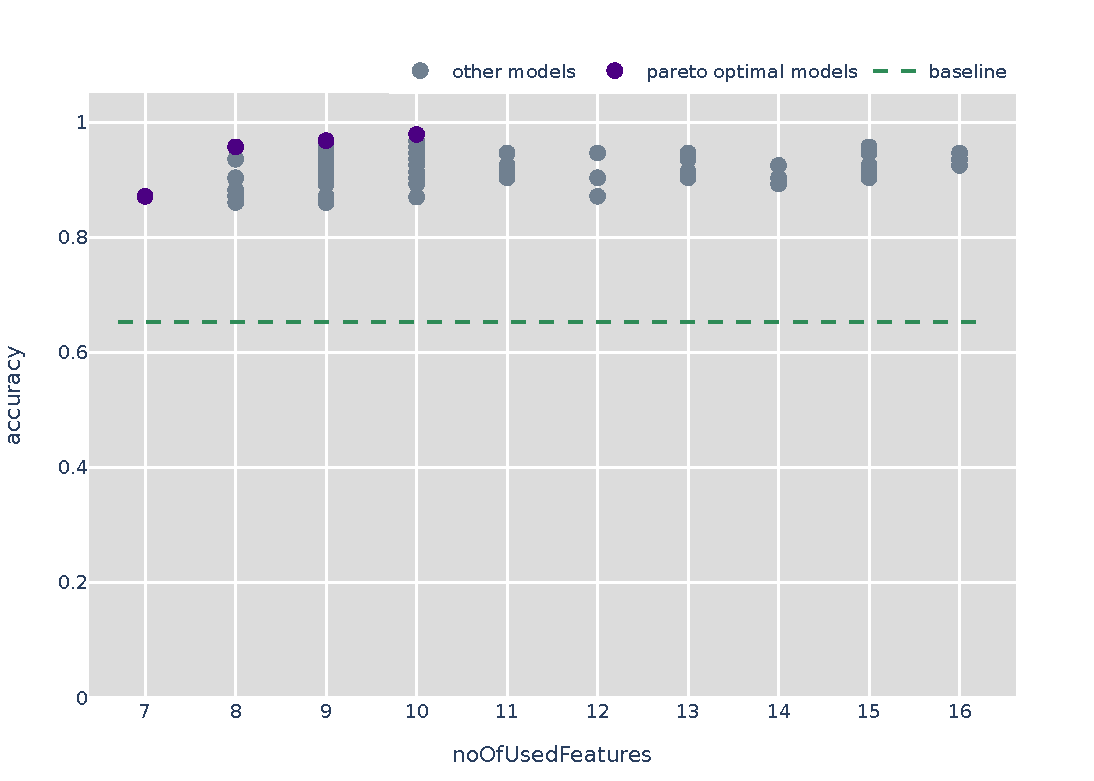
\includegraphics[width=0.85\columnwidth]{figures/genes/paretoFront_TCGA_KIRP_vs_KIRC.pdf}
                \caption{`TCGA\_KIRP\_vs\_KIRC' data set.}\label{fig:paretoKIRPvsKIRC}
        \end{subfigure}
        \hfill
        \begin{subfigure}{\textwidth}
                \centering
                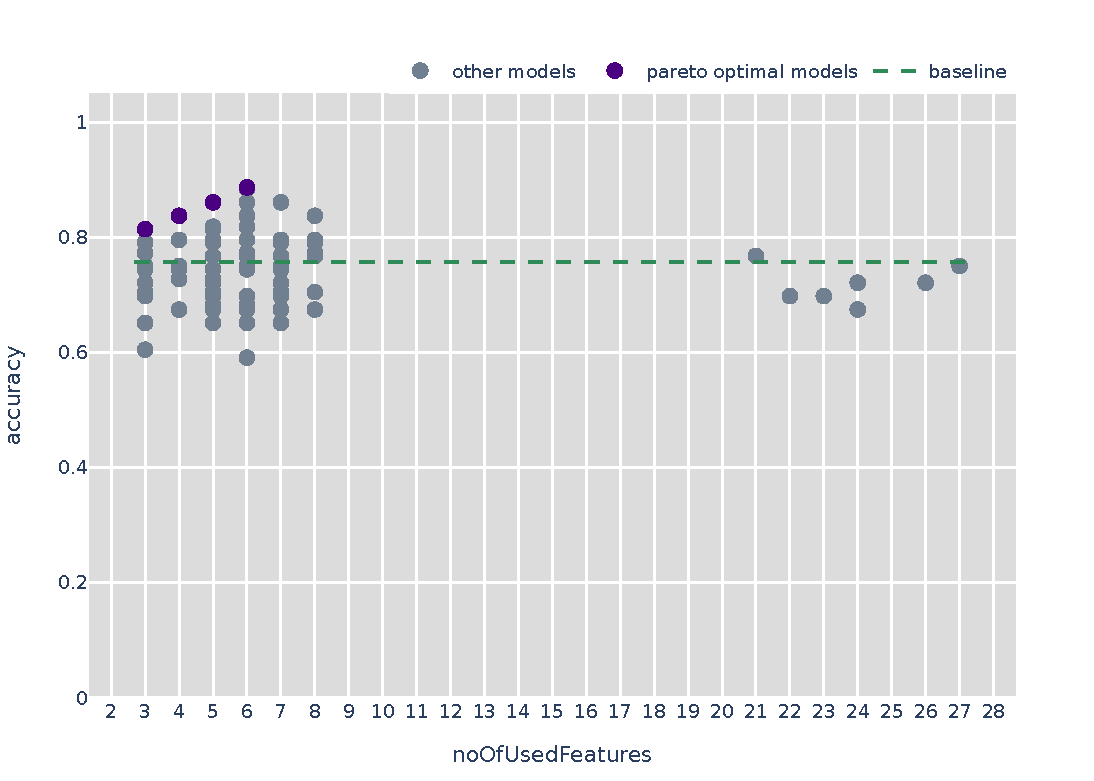
\includegraphics[width=0.85\columnwidth]{figures/genes/paretoFront_TCGA_COAD_vs_READ.pdf}
                \caption{`TCGA\_COAD\_vs\_READ' data set.}\label{fig:paretoCOADvsREAD}
        \end{subfigure}
        \caption{Accuracy-compactness plot for the cross-validation folds of two different RNA-seq data set.}\label{fig:genePareto}
\end{figure}

The resulting \(SCM_{DNF}\) configuration with \(p=1\) and \(minConjSize=10\) was now once more applied to the RNA-seq data sets.
This version of the SCM successfully creates very sparse classifiers (see \autoref{tab:geneCompact}) with in general high accuracies, way above the data's baselines, like visualized on
the example of `TCGA\_KIRP\_vs\_KIRC' in \autoref{fig:paretoKIRPvsKIRC}.
The only exception to this is the `TCGA\_COAD\_vs\_READ' data set, as illustrated in \autoref{fig:paretoCOADvsREAD}, where only the accuracies of 46.3\% of all
classifiers are actually above the baseline.
While the SCM is still able to classify the test samples with a reasonable accuracy through decision rules like
`\texttt{IF (EPHA3|2042 > 666.5 AND ADORA2B|136 > 305.5 AND ACO1|48 > 2297.5) OR (ELAVL2|1993 > 209 AND DDC|1644\\< 5461.5 AND ABCA4|24 < 8.5) THEN class `Rectum Adenocarcinoma'}',
it generally fails to a provide good classifications on unknown training samples.
I assume this is because of the high similarity of the two classes, as the examined tumors are both adenocarcinomas
and even located in similar, adjacent tissues.

\begin{table}[ht]
        \centering
        \caption{Summary of differentially expressed genes in the RNA-seq data sets.}\label{tab:geneGene}
        \begin{tabular}{lll}
                \toprule
                data set & class & comparatively high expressed genes \\
                \midrule
                \multirow{2}{*}{KICH\_vs\_KIRC} & KICH & NDUFS7 \\
                & KIRC & RPL39, MALAT1, ACO1 \\
                \specialrule{0pt}{0.8pc}{0pc}
                \multirow{2}{*}{KICH\_vs\_KIRP} & KICH & STAP1, ATP6V0D2, CLCNKB, ARMC4  \\
                & KIRP & CACNA1E, FZD4 \\
                \specialrule{0pt}{0.8pc}{0pc}
                \multirow{2}{*}{KIRP\_vs\_KIRC} & KIRP & FLRT3, GPS1, ACCN3, ATG2A, FGFR3 \\
                & KIRC & ELTD1, PHKA2, BNC1, CAPZA2, BMI1 \\
                \specialrule{0pt}{0.8pc}{0pc}
                \multirow{2}{*}{CHOL\_vs\_LIHC} & CHOL & CAPN6 \\
                & LIHC & APOE, MEA1, CDKN2D \\
                \specialrule{0pt}{0.8pc}{0pc}
                \multirow{2}{*}{CHOL\_vs\_PAAD} & CHOL & ASGR2, ACADM \\
                & PAAD & PTPRN \\
                \specialrule{0pt}{0.8pc}{0pc}
                \multirow{2}{*}{LIHC\_vs\_PAAD} & LIHC & ALDH4A1 \\
                & PAAD & EDN3 \\
                \specialrule{0pt}{0.8pc}{0pc}
                \multirow{2}{*}{COAD\_vs\_READ} & COAD & / \\
                & READ & EPHA3, ADORA2B, ACO1, ELAVL2, HOXD12 \\
                \bottomrule
        \end{tabular}
\end{table}

% Interpretation of the Results - WHAT DOES IT ALL MEAN?
To identify mutated genes, the feature histograms \autoref{fig:histKICHvsKIRC} to \autoref{fig:histCOADvsREAD},
the ray histograms, the constructed pareto-optimal classification rules, as well as the classifiers that are obtained when using all samples for training,
can be assessed.
In \autoref{tab:geneGene} all genes that each occur in at least
one histogram and additionally in at least one of the just mentioned classification rules are aggregated.
Hence, these genes are classified as relevant and sorted them in to their according classes, using the classifiers and ray histograms.

% 1. What do the genes mean? -> look for sth like "Patients who have pancreatic ductal adenocarcinoma show an overexpression of A1BG in pancreatic juice.[6]"
% 2. What do the numbers mean? Is 100 much? What does it mean? Maybe: What's the normal value? -- normalized number of reads that were successfully mapped to this gene
This analysis of the RNA-seq gene expressions revealed some genes, like \texttt{ATP6V0D2} and \texttt{CLCNKB}, that are actually known for being present in striking levels
in those corresponding cancer subtypes~\citep{zhou}.
However the vast majority of the significant gene expressions are actually not really associated to these specific cancer subtypes by prior research.
This results in my conclusion, that genes with very differential expressions in cancerous and benign cells, like the ones listed by~\cite{tcga13},
are usually not the ones that are identified as significant when comparing different, yet still quite similar, cancer subtypes.
Therefore I do in fact not classify the found genes to be extremely cancer promoting, but instead
to be those genes, that make up a tumor's subtleties.
\chapter{Discussion and Conclusion}\label{ch:conclusion}
% What was done?, What are the outcomes?

% general
My extended SCM is capable of handling numerical, as well as nominal, features effortlessly,
which greatly expands the ensemble of the algorithm's possible use cases.
In general, I optimized the algorithm regarding many different aspects, like the optimal placement
of thresholds or the appropriate utilization of tie situations.
Cross-validation experiments revealed that these efforts indeed payed off and resulted in a robustified SCM,
that is able to generate classifiers that are both, sparse and high-performant on independent test samples.

% optimizations der features waren super
The short computation times of my optimized algorithm moreover enable it to process even high-dimensional genetic data sets.
In this use case the SCM's ability to filter crucial features from irrelevant ones and form those
into easily interpretable decision rules is strongly needed, in order to provide understandable scientific insights.
In the end, my \(SCM_{DNF}\) was capable of identifying the differences between various subtypes of cancer
from the TCGA with an average accuracy of 91.52\%.

% DNF
The use of a disjunction of conjunctions, as done by the \(SCM_{DNF}\), turned out to be especially helpful 
on low-dimensional data sets.
Data sets with disjunct decision regions, like \autoref{fig:twoReg} and \autoref{fig:crossP},
particularly benefit from the extended \(SCM_{DNF}\), as those can now be classified with models, that
truly fit their underlying structures.
Yet also the UCI data in \autoref{sec:uci} benefit from the use of multiple disjunct conjunctions.
In the specific case of the `chess' data set, the average number of conjunctions per classification rule being 2.137 indicates,
that the second conjunction within the DNF is quite necessary to obtain good classification results here.

% on high-dimensional data
Even on high-dimensional data, like in \autoref{sec:geneticData}, the \(SCM_{DNF}\) can often outperform the \(SCM_{conj}\).
However usually only a very small improvement can be achieved here and a suitable parameter 
configuration, especially the appropriate choice of the \(minConjSize\), is required.
In case of a too low minimum conjunction size, the use of a disjunction of conjunctions
actually impairs the classifier's generalizability.
On the other hand side, a too high \(minConjSize\) leads to a 
resulting classification rule that actually consists of only a single conjunction and
therefore the same result as the simpler \(SCM_{conj}\).
In case of the RNA-seq data sets, this consideration resulted in the selection of \(minConjSize = 10\),
leading to slightly improved accuracies as examined in \autoref{tab:geneMCS} and \autoref{tab:geneP}.
Yet, the \(SCM_{DNF}\) provides no major improvement to the model's accuracy here and in five
of the seven data sets the possibility of the \(SCM_{DNF}\) to use multiple conjunctions is
not really used at all (see \autoref{tab:geneCompact}).
This can be reasoned by the vast amount of features to choose the optimal base classifiers from and
by the fact, that gene expression data usually does not contain disjunct decision regions.
In general, two different cancer types will either have similar expression levels for a \(gene_a\)
or one type will a higher expression than the other.
Therefore rules like `\texttt{IF \(gene_a < \alpha\) or \(gene_a > \beta\) THEN class 1}' do usually not occur in this use case.

\begin{table}[ht]
    \centering
    \caption{Average amounts of utilized rays, features and conjunctions within the classification rules of the final \(SCM_{DNF}\).}\label{tab:geneCompact}
    \begin{tabular}{llll}
            \toprule
            data set & |rays| & |features| & |conjunctions| \\
            \midrule
            KICH\_vs\_KIRC & 4.19 & 4.19 & 1.058 \\
            KICH\_vs\_KIRP & 3.84 & 3.84 & 1.045 \\
            KIRP\_vs\_KIRC & 10.34 & 10.34 & 2.033 \\
            CHOL\_vs\_LIHC & 3.13 & 3.13 & 1.0 \\
            CHOL\_vs\_PAAD & 2.1 & 2.1 & 1.0 \\
            LIHC\_vs\_PAAD & 1.85 & 1.85 & 1.0 \\
            COAD\_vs\_READ & 6.73 & 6.73 & 1.778 \\
            \bottomrule
    \end{tabular}
\end{table}

% conclusion
However, even a classifier resulting from the \(SCM_{DNF}\), that consists of only one conjunction,
does in general still match the classifier of an equivalent \(SCM_{conj}\).
Meaning, that the \(SCM_{DNF}\) does represent a good chance for the set covering machine
to classify even complex scattered data, yet still delivers a feasible result, i.e.\ the one
of the \(SCM_{conj}\), in case of only one decision region.
The major downside of the \(SCM_{DNF}\) however stays the additional effort that needs to
be put in the careful adjustment of the \(minConjSize\) hyper-parameter, that is not needed
when using a \(SCM_{conj}\).
Yet, if done properly, the \(SCM_{DNF}\) does in general not only have a superior accuracy on its training
data, but also the same, or often an even higher, generalizability than the equivalent \(SCM_{conj}\).

\backmatter%%%%%%%%%%%%%%%%%%%%%%%%%%%%%%%%%%%%%%%%%%%%%%%%%%%%%%%%%%%%%%%%%%%%%%%%%%%%%%%%%

\bibliographystyle{unsrtnat}
\bibliography{bibliography}

\listoffigures
\listoftables

\appendix
\chapter{Appendix}\label{ch:appendix}

%%%%%%%%%%%%%%%%%%%%%%%%%%%%%%%%%%%%%%%%%%%%%%%%%%%%%%%%%%%%%%%%%%%%%%%%%%%%%%%%%%%%%%%%%%%%
\section{Tables}

Listing of all tables used in \autoref{subsec:studySCM}.

\begin{table}[H]
    \centering
    \caption{Accuracies of the SCM on RNA-seq data with different values of the \(minConjSize\) parameter. \(p=1\) was used in all cases.}\label{tab:geneMCS}
    \begin{tabular}{lllllll}
        \toprule
        data set & SCM type & \(mcs=1\) & \(mcs=2\) & \(mcs=5\) & \(mcs=10\) & \(mcs=20\) \\
        \midrule
        \multirow{2}{*}{KICH\_vs\_KIRC} & \(SCM_{conj}\) & 0.957 & 0.956 & 0.958 & 0.96 & 0.958 \\
        & \(SCM_{DNF}\) & 0.963 & 0.963 & 0.962 & 0.96 & 0.958 \\
        \specialrule{0pt}{0.8pc}{0pc}
        \multirow{2}{*}{KICH\_vs\_KIRP} & \(SCM_{conj}\) & 0.918 & 0.918 & 0.917 & 0.92 & 0.923 \\
        & \(SCM_{DNF}\) & 0.924 & 0.925 & 0.919 & 0.92 & 0.923 \\
        \specialrule{0pt}{0.8pc}{0pc}
        \multirow{2}{*}{KIRP\_vs\_KIRC} & \(SCM_{conj}\) & 0.905 & 0.906 & 0.911 & 0.91 & 0.91 \\
        & \(SCM_{DNF}\) & 0.917 & 0.923 & 0.925 & 0.922 & 0.916 \\
        \specialrule{0pt}{0.8pc}{0pc}
        \multirow{2}{*}{CHOL\_vs\_LIHC} & \(SCM_{conj}\) & 0.917 & 0.927 & 0.928 & 0.937 & 0.932 \\
        & \(SCM_{DNF}\) & 0.924 & 0.927 & 0.926 & 0.937 & 0.932 \\
        \specialrule{0pt}{0.8pc}{0pc}
        \multirow{2}{*}{CHOL\_vs\_PAAD} & \(SCM_{conj}\) & 0.921 & 0.929 & 0.937 & 0.933 & 0.931 \\
        & \(SCM_{DNF}\) & 0.929 & 0.936 & 0.937 & 0.933 & 0.931 \\
        \specialrule{0pt}{0.8pc}{0pc}
        \multirow{2}{*}{LIHC\_vs\_PAAD} & \(SCM_{conj}\) & 0.982 & 0.985 & 0.984 & 0.985 & 0.985 \\
        & \(SCM_{DNF}\) & 0.982 & 0.985 & 0.984 & 0.985 & 0.985 \\
        \specialrule{0pt}{0.8pc}{0pc}
        \multirow{2}{*}{COAD\_vs\_READ} & \(SCM_{conj}\) & 0.705 & 0.736 & 0.756 & 0.761 & 0.759 \\
        & \(SCM_{DNF}\) & 0.7 & 0.7 & 0.74 & 0.753 &  0.759 \\
        \midrule
        \multicolumn{2}{c}{avg no of conjunctions} & 5.777 & 4.657 & 2.043 & 1.262 & 1.066 \\ 
        \bottomrule
    \end{tabular}
\end{table}

\begin{table}[H]
    \centering
    \caption{Accuracies of the SCM on RNA-seq data with different values of the penalty parameter \(p\). \(minConjSize = 10\) was used in all cases.}\label{tab:geneP}
    \begin{tabular}{lllllc}
            \toprule
            data set & SCM type & \(p=0.5\) & \(p=1\) & \(p=2\) & \(p=\frac{|\text{`neg.\ samples'}|}{|\text{`pos.\ samples'}|}\)\\
            \midrule
            \multirow{2}{*}{KICH\_vs\_KIRC} & \(SCM_{conj}\) & 0.972 & 0.96 & 0.952 & 0.947 \\
            & \(SCM_{DNF}\) & 0.977 & 0.96 & 0.953 & 0.968 \\
            \specialrule{0pt}{0.8pc}{0pc}
            \multirow{2}{*}{KICH\_vs\_KIRP} & \(SCM_{conj}\) & 0.919 & 0.92 & 0.905 & 0.907 \\
            & \(SCM_{DNF}\) & 0.923 & 0.92 & 0.906 & 0.919 \\
            \specialrule{0pt}{0.8pc}{0pc}
            \multirow{2}{*}{KIRP\_vs\_KIRC} & \(SCM_{conj}\) & 0.891 & 0.91 & 0.902 & 0.896 \\
            & \(SCM_{DNF}\) & 0.904 & 0.922 & 0.918 & 0.914 \\
            \specialrule{0pt}{0.8pc}{0pc}
            \multirow{2}{*}{CHOL\_vs\_LIHC} & \(SCM_{conj}\) & 0.935 & 0.937 & 0.925 & 0.845 \\
            & \(SCM_{DNF}\) & 0.935 & 0.937 & 0.925 & 0.919 \\
            \specialrule{0pt}{0.8pc}{0pc}
            \multirow{2}{*}{CHOL\_vs\_PAAD} & \(SCM_{conj}\) & 0.938 & 0.933 & 0.938 & 0.957 \\
            & \(SCM_{DNF}\) & 0.938 & 0.933 & 0.938 & 0.957 \\
            \specialrule{0pt}{0.8pc}{0pc}
            \multirow{2}{*}{LIHC\_vs\_PAAD} & \(SCM_{conj}\) & 0.982 & 0.985 & 0.985 & 0.985 \\
            & \(SCM_{DNF}\) & 0.982 & 0.985 & 0.985 & 0.985 \\
            \specialrule{0pt}{0.8pc}{0pc}
            \multirow{2}{*}{COAD\_vs\_READ} & \(SCM_{conj}\) & 0.761 & 0.761 & 0.778 & 0.664 \\
            & \(SCM_{DNF}\) & 0.76 & 0.753 & 0.776 & 0.704 \\
            \bottomrule
    \end{tabular}
\end{table}

\begin{table}[H]
    \centering
    \caption{Ratios of sensitivity to specificity when using different \(p\) values on the RNA-seq data sets. The \(SCM_{DNF}\) with \(minConjSize = 10\) was used in all cases.}\label{tab:genePMiddle}
    \begin{tabular}{llc}
            \toprule
            data set & \(p=1\) & \(p=\frac{|\text{`neg.\ samples'}|}{|\text{`pos.\ samples'}|}\) \\
            \midrule
            KICH\_vs\_KIRC & 1.227 & 1.067 \\
            KICH\_vs\_KIRP & 1.229 & 1.1 \\
            KIRP\_vs\_KIRC & 0.888 & 0.98 \\
            CHOL\_vs\_LIHC & 2.021 & 1.491 \\
            CHOL\_vs\_PAAD & 1.212 & 0.988 \\
            LIHC\_vs\_PAAD & 0.991 & 1.003 \\
            COAD\_vs\_READ & 0.207 & 0.709 \\
            \bottomrule
    \end{tabular}
\end{table}

\begin{table}[H]
    \centering
    \caption{Comparison between an \(SCM_{DNF}\) utilizing versus not utilizing ties on the RNA-seq data. The \(SCM_{DNF}\) with \(p=1\) and \(minConjSize = 10\) was used in all cases.}\label{tab:geneTies}
    \begin{tabular}{llllllr}
        \toprule
        data set & used ties? & acc. & |rays| & exec.\ time & RAM & |used ties| \\
        \midrule
        \multirow{2}{*}{KICH\_vs\_KIRC} & no & 0.96 & 4.12 & 303~s & 1,061~GiB & 0 \\
        & yes & 0.961 & 4.08 & 518~s & 1,334~GiB & 0.017 \\
        \specialrule{0pt}{0.8pc}{0pc}
        \multirow{2}{*}{KICH\_vs\_KIRP} & no & 0.923 & 3.75 & 190~s & 543~GiB & 0 \\
        & yes & 0.92 & 3.66 & 298~s & 660~GiB & 0.01 \\
        \specialrule{0pt}{0.8pc}{0pc}
        \multirow{2}{*}{KIRP\_vs\_KIRC} & no & 0.922 & 10.2 & 647~s & 2,383~GiB & 0 \\
        & yes & 0.911 & 8.87 & 1046~s & 2,809~GiB & 0.132 \\
        \specialrule{0pt}{0.8pc}{0pc}
        \multirow{2}{*}{CHOL\_vs\_LIHC} & no & 0.94 & 3.36 & 221~s & 728~GiB & 0 \\
        & yes & 0.935 & 3.27 & 373~s & 917~GiB & 0.007 \\
        \specialrule{0pt}{0.8pc}{0pc}
        \multirow{2}{*}{CHOL\_vs\_PAAD} & no & 0.93 & 2.1 & 125~s & 257~GiB & 0 \\
        & yes & 0.928 & 2.1 & 168~s & 315~GiB & 0 \\
        \specialrule{0pt}{0.8pc}{0pc}
        \multirow{2}{*}{LIHC\_vs\_PAAD} & no & 0.986 & 1.78 & 135~s & 448~GiB & 0 \\
        & yes & 0.985 & 1.81 & 218~s & 523~GiB & 0 \\
        \specialrule{0pt}{0.8pc}{0pc}
        \multirow{2}{*}{COAD\_vs\_READ} & no & 0.757 & 6.3 & 549~s & 1,789~GiB & 0 \\
        & yes & 0.761 & 5.93 & 901~s & 2,232~GiB & 0.582 \\
        \bottomrule
    \end{tabular}
\end{table}

\clearpage
%%%%%%%%%%%%%%%%%%%%%%%%%%%%%%%%%%%%%%%%%%%%%%%%%%%%%%%%%%%%%%%%%%%%%%%%%%%%%%%%%%%%%%%%%%%%
\section{Histogram Plots}

Listing of all histograms used in \autoref{ch:evaluation}.

\begin{figure}[H]
    \centering
    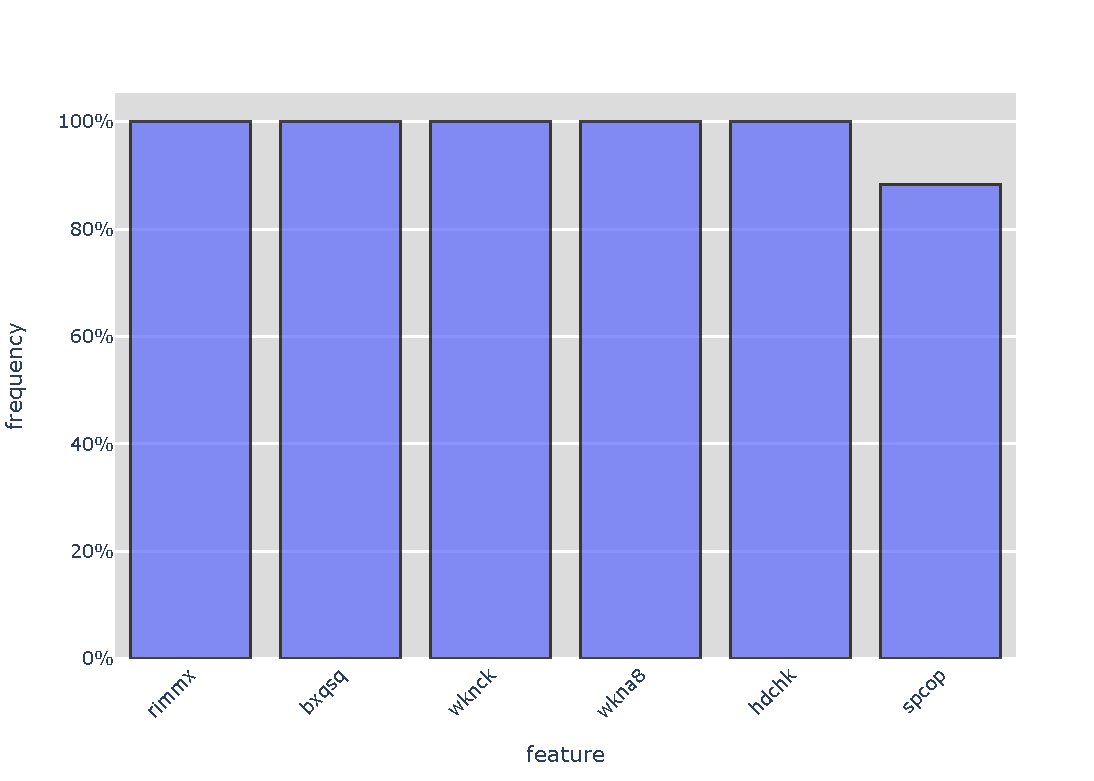
\includegraphics[width=0.8\columnwidth]{figures/chess/featureHistogram.pdf}
    \caption{Histogram of the important features from the `chess' data set.}\label{fig:histChessF}
\end{figure}
\begin{figure}[H]
    \centering
    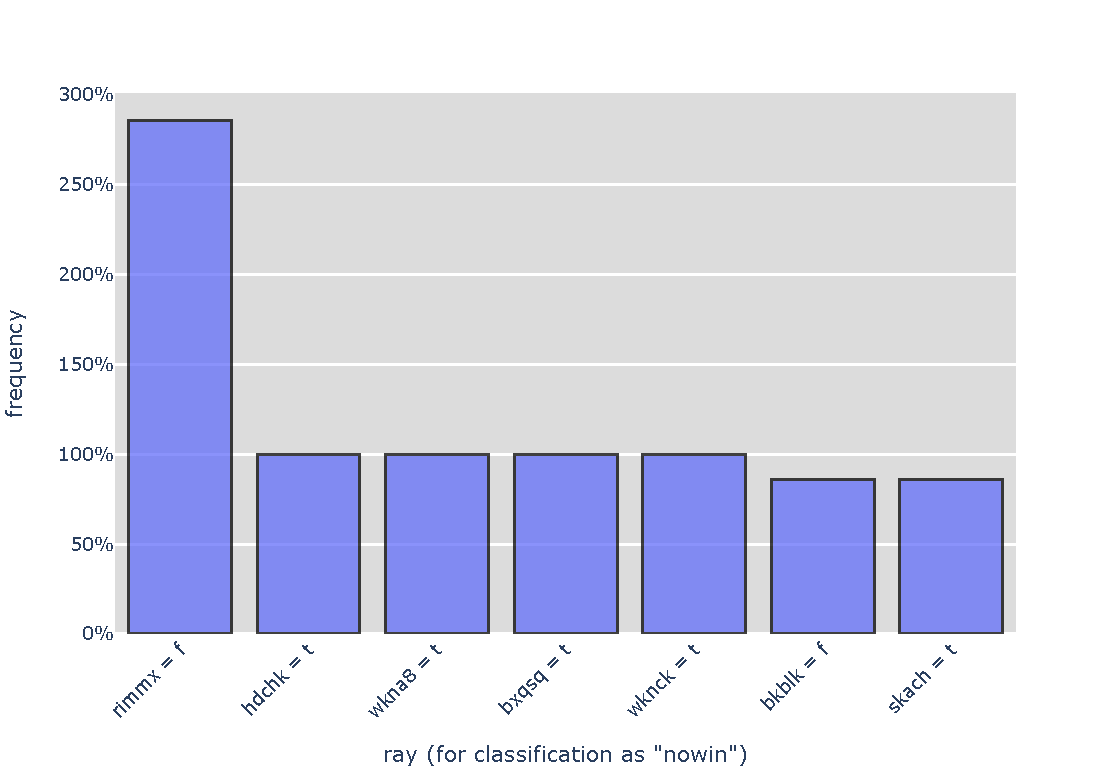
\includegraphics[width=0.8\columnwidth]{figures/chess/raysClass0Histogram.pdf}
    \caption{Histogram of the important class 0 base classifiers from the `chess' data set.}\label{fig:histChessR0}
\end{figure}
\begin{figure}[H]
    \centering
    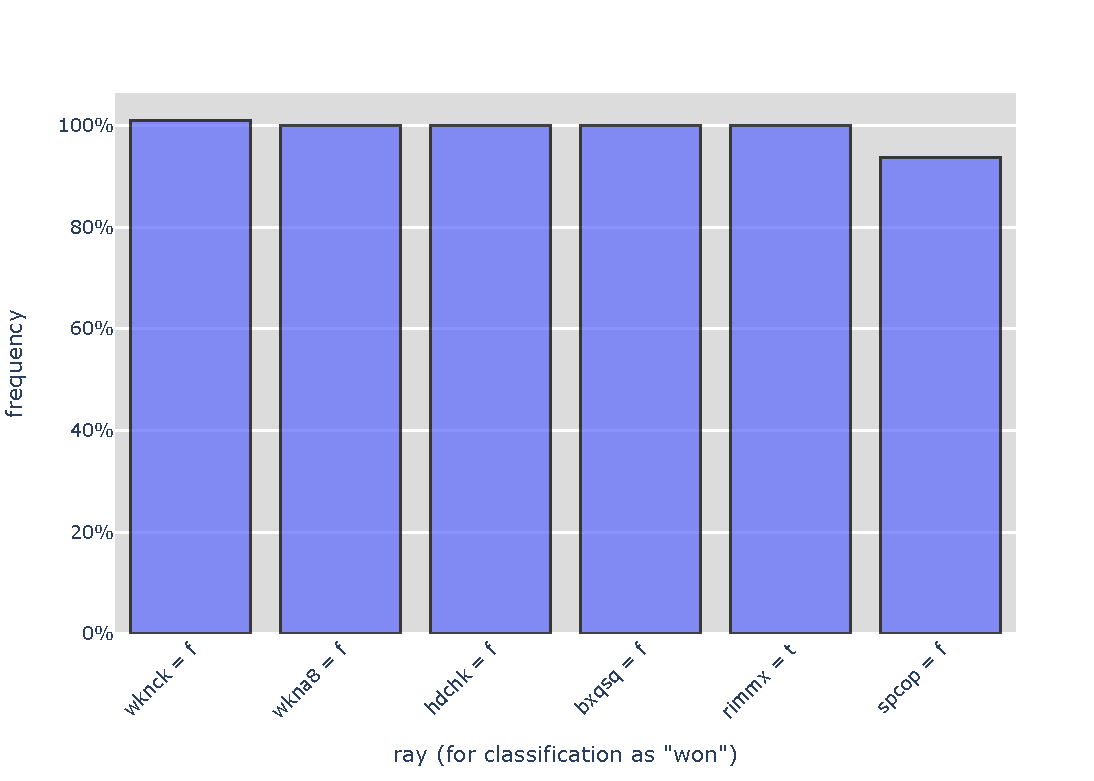
\includegraphics[width=0.9\columnwidth]{figures/chess/raysClass1Histogram.pdf}
    \caption{Histogram of the important class 1 base classifiers from the `chess' data set.}\label{fig:histChessR1}
\end{figure}

\begin{figure}[H]
    \centering
    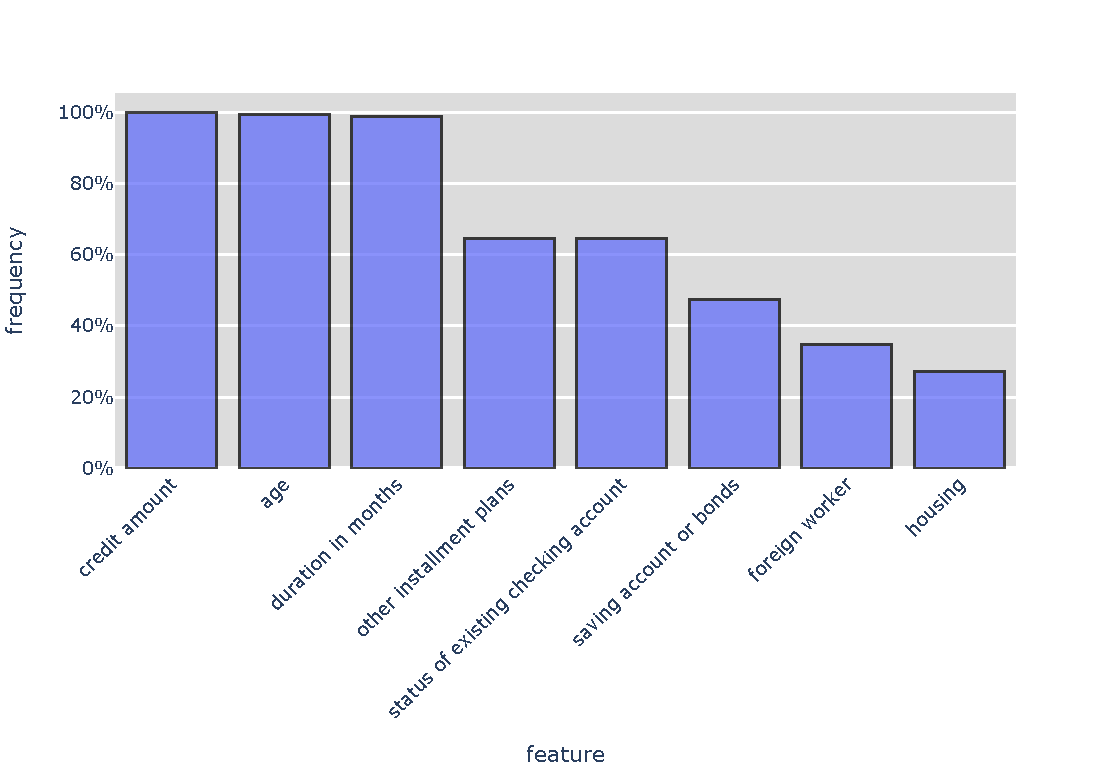
\includegraphics[width=0.9\columnwidth]{figures/german/featureHistogram.pdf}
    \caption{Histogram of the important features from the `german' data set.}\label{fig:histGermanF}
\end{figure}
\begin{figure}[H]
    \centering
    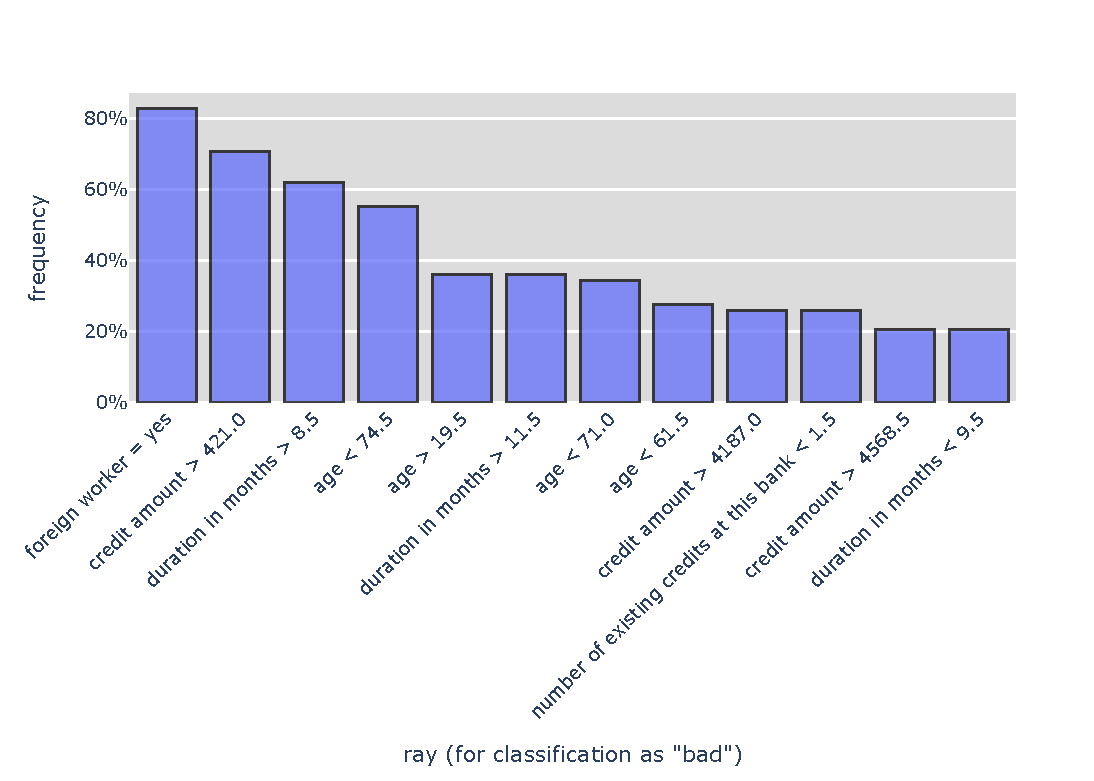
\includegraphics[width=0.9\columnwidth]{figures/german/raysClass0Histogram.pdf}
    \caption{Histogram of the important class 0 base classifiers from the `german' data set.}\label{fig:histGermanR0}
\end{figure}
\begin{figure}[H]
    \centering
    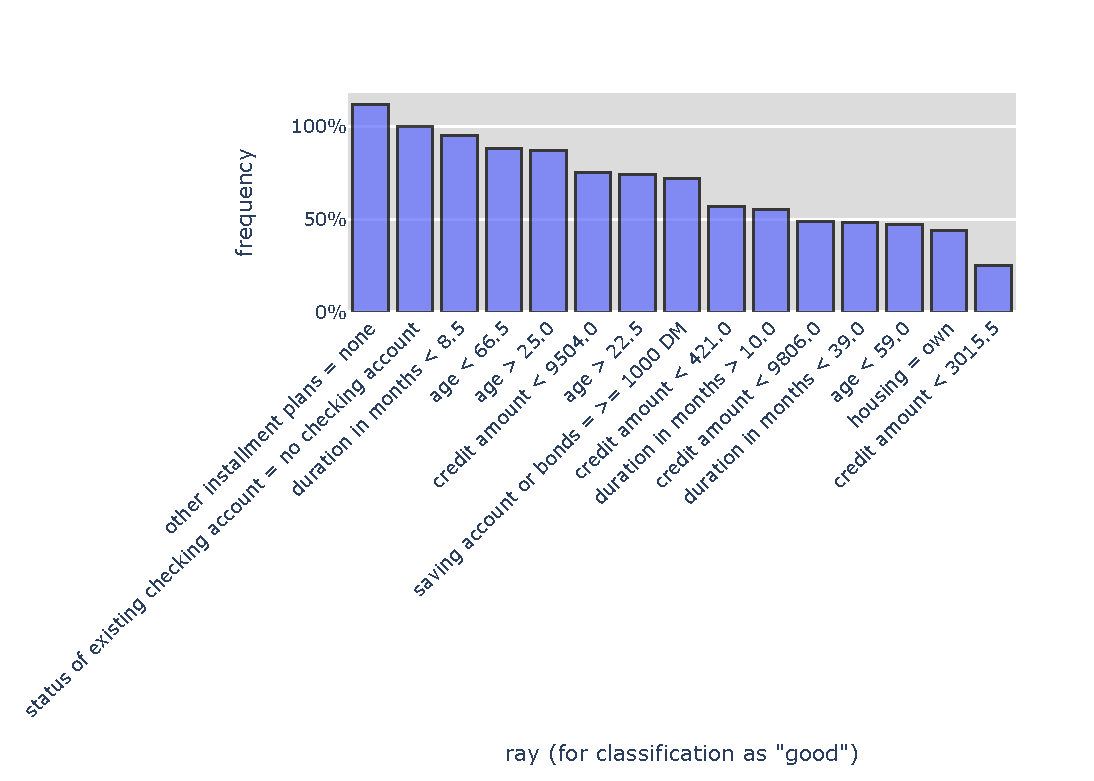
\includegraphics[width=0.9\columnwidth]{figures/german/raysClass1Histogram.pdf}
    \caption{Histogram of the important class 1 base classifiers from the `german' data set.}\label{fig:histGermanR1}
\end{figure}

\begin{figure}[H]
    \centering
    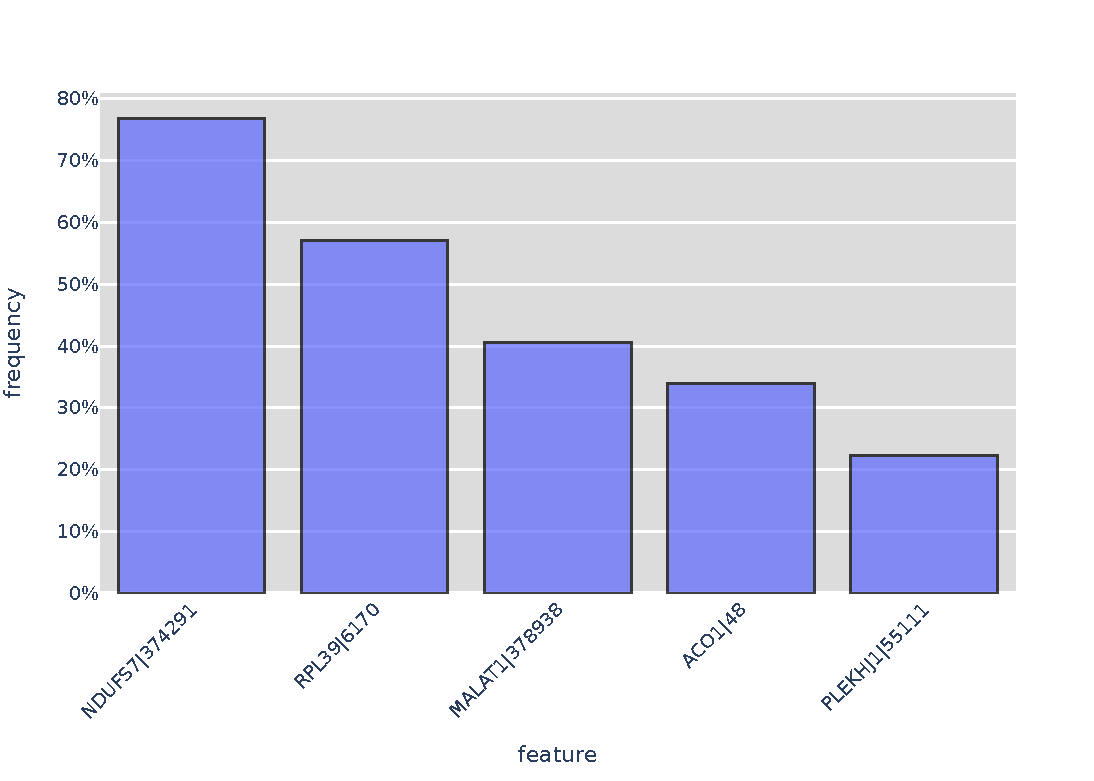
\includegraphics[width=0.9\columnwidth]{figures/genes/featureHistogram_TCGA_KICH_vs_KIRC.pdf}
    \caption{Histogram of the important features from the `KICH\_vs\_KIRC' data set.}\label{fig:histKICHvsKIRC}
\end{figure}
\begin{figure}[H]
    \centering
    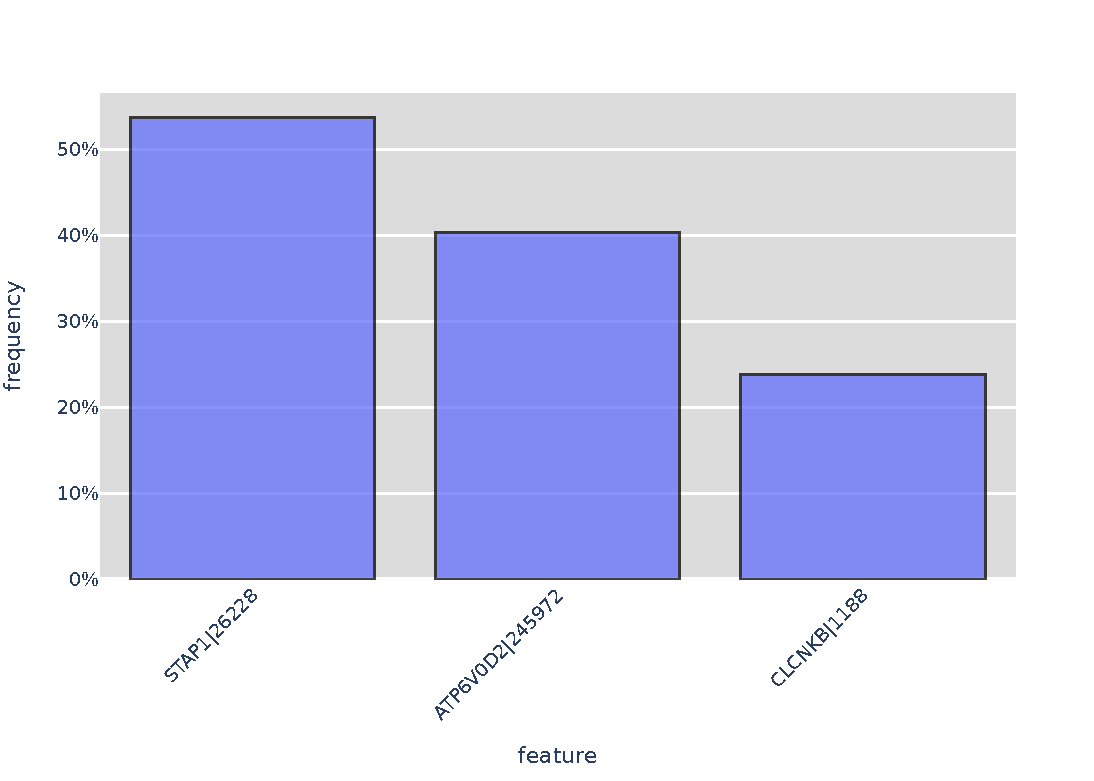
\includegraphics[width=0.9\columnwidth]{figures/genes/featureHistogram_TCGA_KICH_vs_KIRP.pdf}
    \caption{Histogram of the important features from the `KICH\_vs\_KIRP' data set.}\label{fig:histKICHvsKIRP}
\end{figure}
\begin{figure}[H]
    \centering
    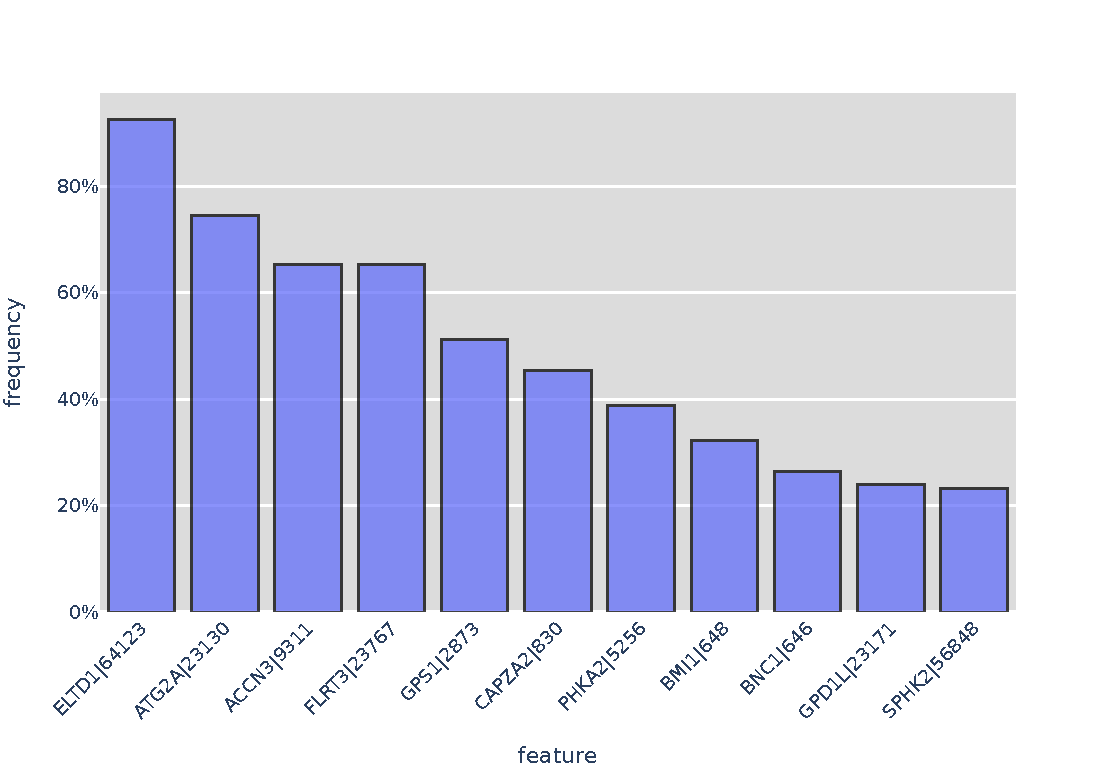
\includegraphics[width=0.9\columnwidth]{figures/genes/featureHistogram_TCGA_KIRP_vs_KIRC.pdf}
    \caption{Histogram of the important features from the `KIRP\_vs\_KIRC' data set.}\label{fig:histKIRPvsKIRC}
\end{figure}
\begin{figure}[H]
    \centering
    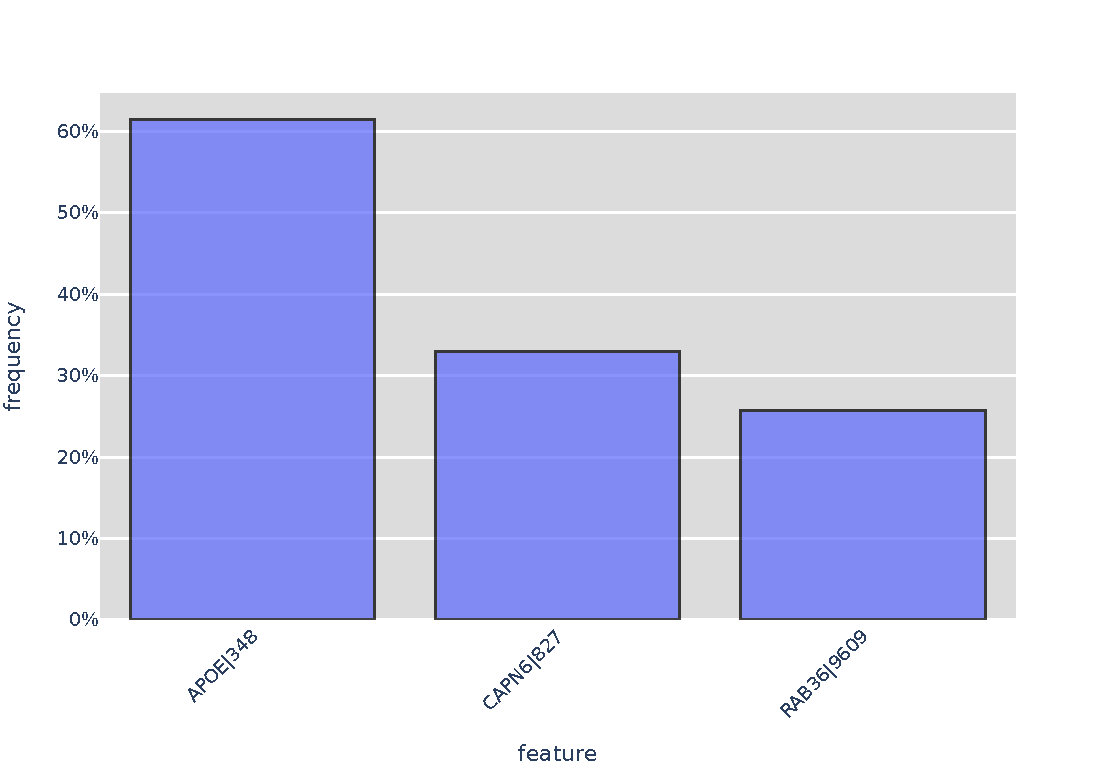
\includegraphics[width=0.9\columnwidth]{figures/genes/featureHistogram_TCGA_CHOL_vs_LIHC.pdf}
    \caption{Histogram of the important features from the `CHOL\_vs\_LIHC' data set.}\label{fig:histCHOLvsLIHC}
\end{figure}
\begin{figure}[H]
    \centering
    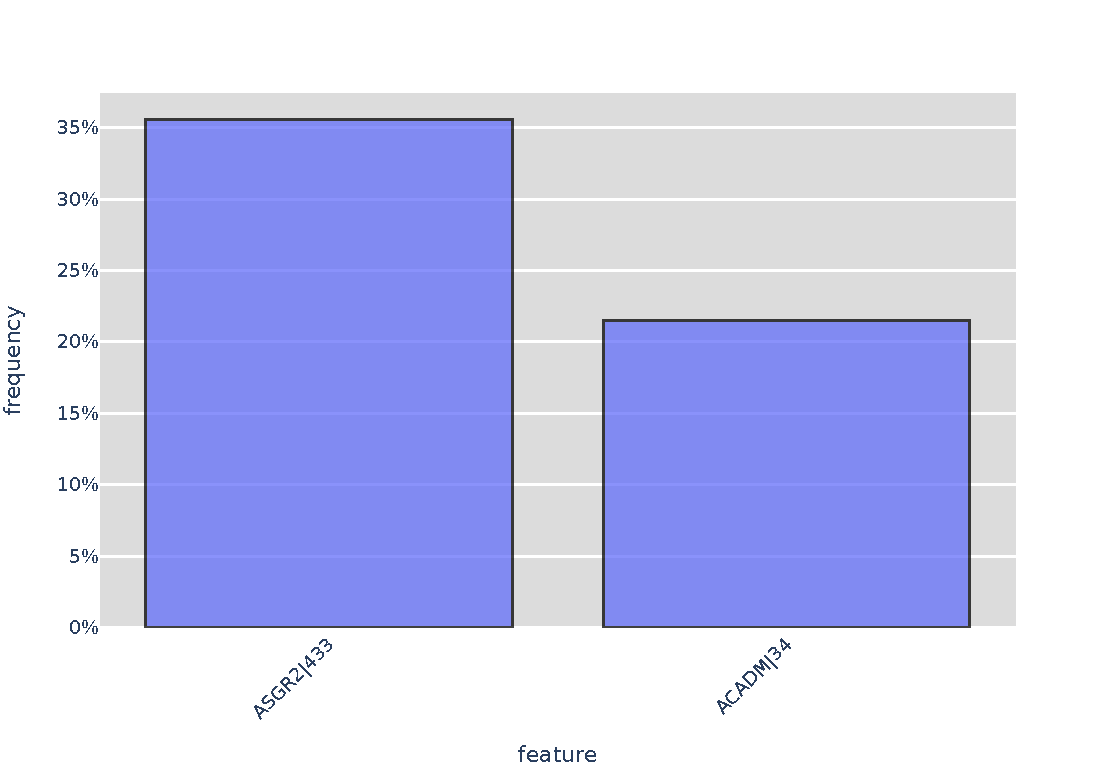
\includegraphics[width=0.9\columnwidth]{figures/genes/featureHistogram_TCGA_CHOL_vs_PAAD.pdf}
    \caption{Histogram of the important features from the `CHOL\_vs\_PAAD' data set.}\label{fig:histCHOLvsPAAD}
\end{figure}
\begin{figure}[H]
    \centering
    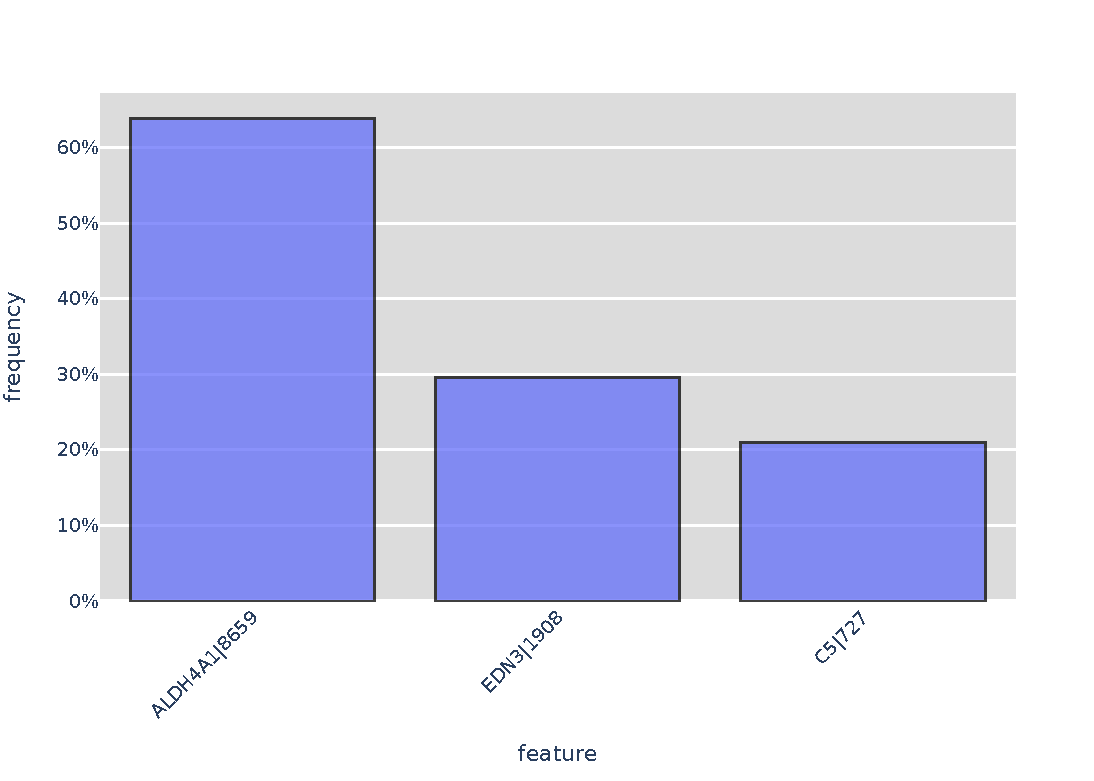
\includegraphics[width=0.9\columnwidth]{figures/genes/featureHistogram_TCGA_LIHC_vs_PAAD.pdf}
    \caption{Histogram of the important features from the `LIHC\_vs\_PAAD' data set.}\label{fig:histLIHCvsPAAD}
\end{figure}
\begin{figure}[H]
    \centering
    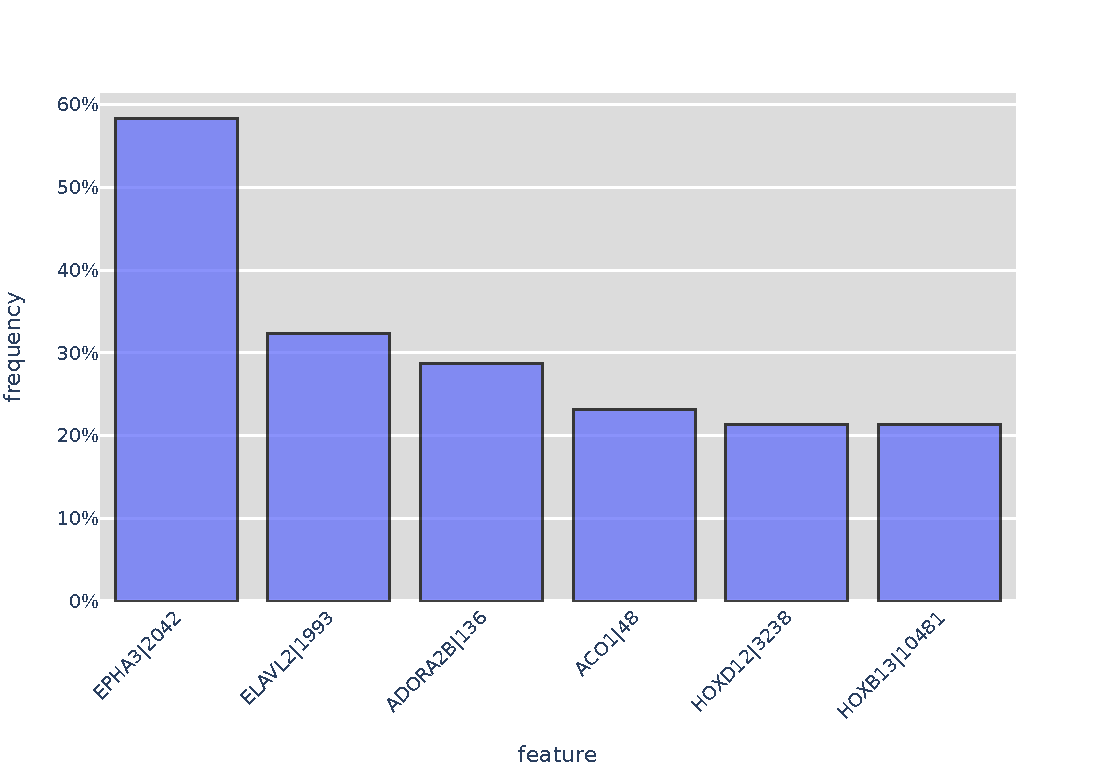
\includegraphics[width=0.9\columnwidth]{figures/genes/featureHistogram_TCGA_COAD_vs_READ.pdf}
    \caption{Histogram of the important features from the `COAD\_vs\_READ' data set.}\label{fig:histCOADvsREAD}
\end{figure}

\clearpage
%%%%%%%%%%%%%%%%%%%%%%%%%%%%%%%%%%%%%%%%%%%%%%%%%%%%%%%%%%%%%%%%%%%%%%%%%%%%%%%%%%%%%%%%%%%%
\section{Julia Source Code}

Listing of all Julia algorithms used in the \autoref{ch:julia} to \autoref{ch:evaluation}.

% chapter 3
\jlinputlisting[label={julia:calcScore},caption={Algorithm calculating a feature's usefulness score.}]{source_code/calc_score.jl}
\jlinputlisting[label={julia:buildConj},caption={Algorithm constructing a conjunction out of multiple optimal base classifiers.}]{source_code/build_conjunction.jl}
\jlinputlisting[label={julia:toString},caption={Algorithm to convert a base classifier, conjunction or disjunction to string using multiple dispatch and recursiveness.}]{source_code/to_string.jl}
\jlinputlisting[label={julia:boolLabels},caption={Algorithm updating a data frame by replacing the labels (usually Strings) by the Boolean classes `true' and `false'. Returning the set of original labels.}]{source_code/bool_labels.jl}
\jlinputlisting[label={julia:findBaseClassifier},caption={Algorithm comparing the return values of \texttt{inspect\_single\_feature} to find the optimum base classifier.}]{source_code/find_ray.jl}

% chapter 4
\jlinputlisting[label={julia:buildDnf},caption={Algorithm constructing a disjunction out of multiple optimal conjunctions.}]{source_code/build_dnf.jl}
\jlinputlisting[label={julia:classify},caption={Algorithm predicting the label of a sample based on a classification rule.}]{source_code/classify.jl}
\jlinputlisting[label={julia:tiesCollect1},caption={Expanding the \texttt{inspect\_single\_feature (NominalFeature)} and \texttt{find\_border} algorithm to collect ties.}]{source_code/ties/collect1.jl}
\jlinputlisting[label={julia:tiesCollect2},caption={Expanding the \texttt{inspect\_single\_feature (NumericalFeature)} algorithm to collect ties.}]{source_code/ties/collect2.jl}
\jlinputlisting[label={julia:tiesCollect3},caption={Expanding the \texttt{find\_base\_classifier} algorithm to collect ties.}]{source_code/ties/collect3.jl}
\jlinputlisting[label={julia:buildConjTies},caption={Expansion of the \texttt{build\_conjunction} algorithm that uses and collects ties.}]{source_code/ties/build_conj.jl}
\jlinputlisting[label={julia:buildDnfTies},caption={Expanding the \texttt{build\_dnf} algorithm to use ties.}]{source_code/ties/build_dnf.jl}

% chapter 5
\jlinputlisting[label={julia:loadCsv},caption={Algorithm parsing fixed width strings from a CSV file into regular strings.}]{source_code/load_csv.jl}
\jlinputlisting[label={julia:inspectNumerical},caption={Algorithm identifying the optimal ray on a specific numerical feature.}]{source_code/inspect_single_feature_num.jl}
\jlinputlisting[label={julia:findBorder},caption={Algorithm identifying the optimal ray for a specific operator on a specific numerical feature.}]{source_code/find_border.jl}
\jlinputlisting[label={julia:preventRecorr},caption={Algorithm preventing the SCM to choose rays that would override previously selected rays.}]{source_code/prevent_recorr.jl}
\jlinputlisting[label={julia:thresholdInbetween},caption={Algorithmic extension to maximize a ray's margins.}]{source_code/threshold_inbetween.jl}
\jlinputlisting[label={julia:inspectNominal},caption={Algorithm identifying the optimal base classifier on a specific nominal feature.}]{source_code/inspect_single_feature_nom.jl}

% chapter 6
\jlinputlisting[label={julia:cv},caption={Most important parts of the \(m \times n\) cross-validation algorithm.}]{source_code/cross_validation.jl}
\jlinputlisting[label={julia:paretoFront},caption={Algorithm computing all models on the first pareto front.}]{source_code/pareto_front.jl}
\jlinputlisting[label={julia:loadRData},caption={Algorithm to load the modified TCGA data sets from~\cite{lausser20}.}]{source_code/load_rdata.jl}

\cleardoublepage%
\clearpairofpagestyles%
\declaration%

\end{document}